\chapter{Gait Watch and Force Plate signals processing}
\label{ch:GWandFP}

\section{Introduction and chapter's structure}
Along this chapter we will introduce the protocol used to obtain the Gait Watch and Force Plate signals as well as the developed software to synchronise and analyse the signals that characterise the anticipatory postural adjustments before gait.

On the one hand, we will carry out the synchronisation between the signal from inertial sensors (Gait Watch) and the force signals from the platform. It's very important for comparing both devices, determining the differences and similarities and finally resolving if we can obtain the same information from both systems.

On the other hand, we’ll analyse the most interesting signals to characterise the APAs, obtaining the parameters of them which may be of interest.


\section{Data gathering Protocol}
Prior to start of data gathering, it’s necessary to set up the protocol for procedure that patients have to carry out while the data are recorded. The establishing of this procedure is very important so that the synchronisation works properly because we have to identify a clear movement in both signals to match one signal with the other at the same time.
In addition, the realised movements must be representatives to obtain conclusive data which help us to extract characteristics for the purpose of identify differences between patients and control subjects subsequently.

The steps followed by the patients are detailed hereafter:

1.	Subject stands in front of the Force Plate.

2.	Gait watch record starts for data gathering.

3.	Force plate record starts for data gathering.

4.	Subject makes a step onto the platform.

5.	Subject stands on the platform a variable time between 2 and 10 seconds.

6.	Subject makes some step  forward and turns left to stand in front of the platform again.

This procedure is repeated ten times by each subject in order to characterise better the movement made.
It’s important to clarify that the GaitWatch recording contains all these ten episodes ( in other cases more) and the platform recording only contains one episode each. So, this is a fact that we have to consider to do the synchronisation.

\section{Synchronisation}

\subsection{Introduction and chapter's structure}
One of the most important aspects whether you have data acquired from multiples devices or channels is the synchronisation. If these data are not appropriately correlated or synchronised, the analysis and conclusions from your use will be erroneous. Also, it’s very important to do all automatically when you have a data on a broad scale.
Therefore, the following sections explain how the information has been obtained and processed automatically, as well as what features have been calculated to characterise the movements of the patients and to carry out the synchronisation between the Force Plate signals and GaitWatch signals. This content is superficially depicted in \ref{fig:diagramSynchronisation}.

\subsection{Design of developed code  in Matlab}
\subsubsection{Selection, reading and obtaining of information from the excel file}
All patients data, that is, the different files have been generated after the gathering (  of the force plate as well as Gait Watch), gathering date, duration of the experiment and other observations are saved in a Excel file. 

In order to automate all as much as possible, the code is in charge of extraction of the necessary data (files names) to carry out the appropriate calculations for each patient. This is done once the Excel file has been selected, thus, it have to have a specific structure to be able to read the data correctly.

At the end of this fraction of code, we save all file names of both systems (force plate and Gait Watch) corresponding to each patient, in order to access and extract them posteriorly.

\begin{figure}[H]
	\centering
	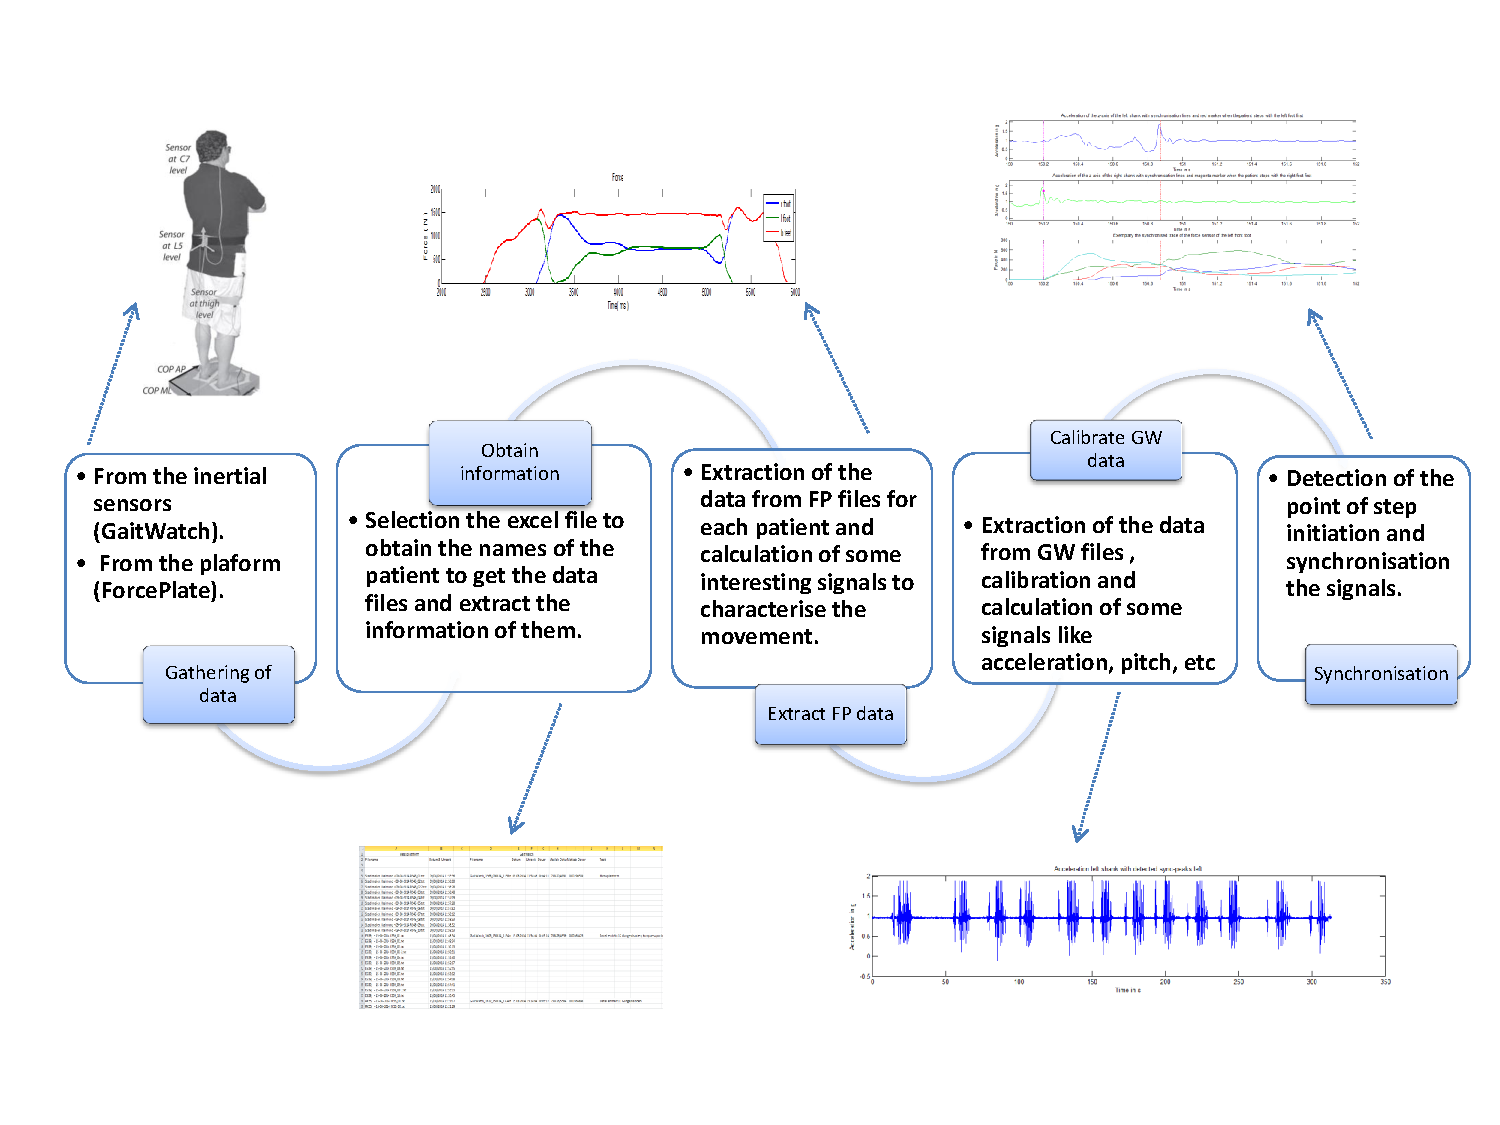
\epsfig{file=imagenes/diagramSynchronisation.pdf, width=16cm}
	\caption{Diagram of the Synchronisation's progress.}
	\label{fig:diagramSynchronisation}
\end{figure}


\subsubsection{Extraction of the forceplate data}
As we said before, the  force plate data files are recorded independently each others, that is, there is a *.txt file for each repeat.
Each file contains the force data of the toes and heels of both feet. It really realises a distribution of the sensors to cover these four segments\ref{fig:Force4signals}. Every measure is obtained for each point of time according to the sample frequency. Also, this file contains the force data from each cell that is part of platform in each frame\ref{fig:pseudocolor}.

\begin{figure}[H]
	\centering
	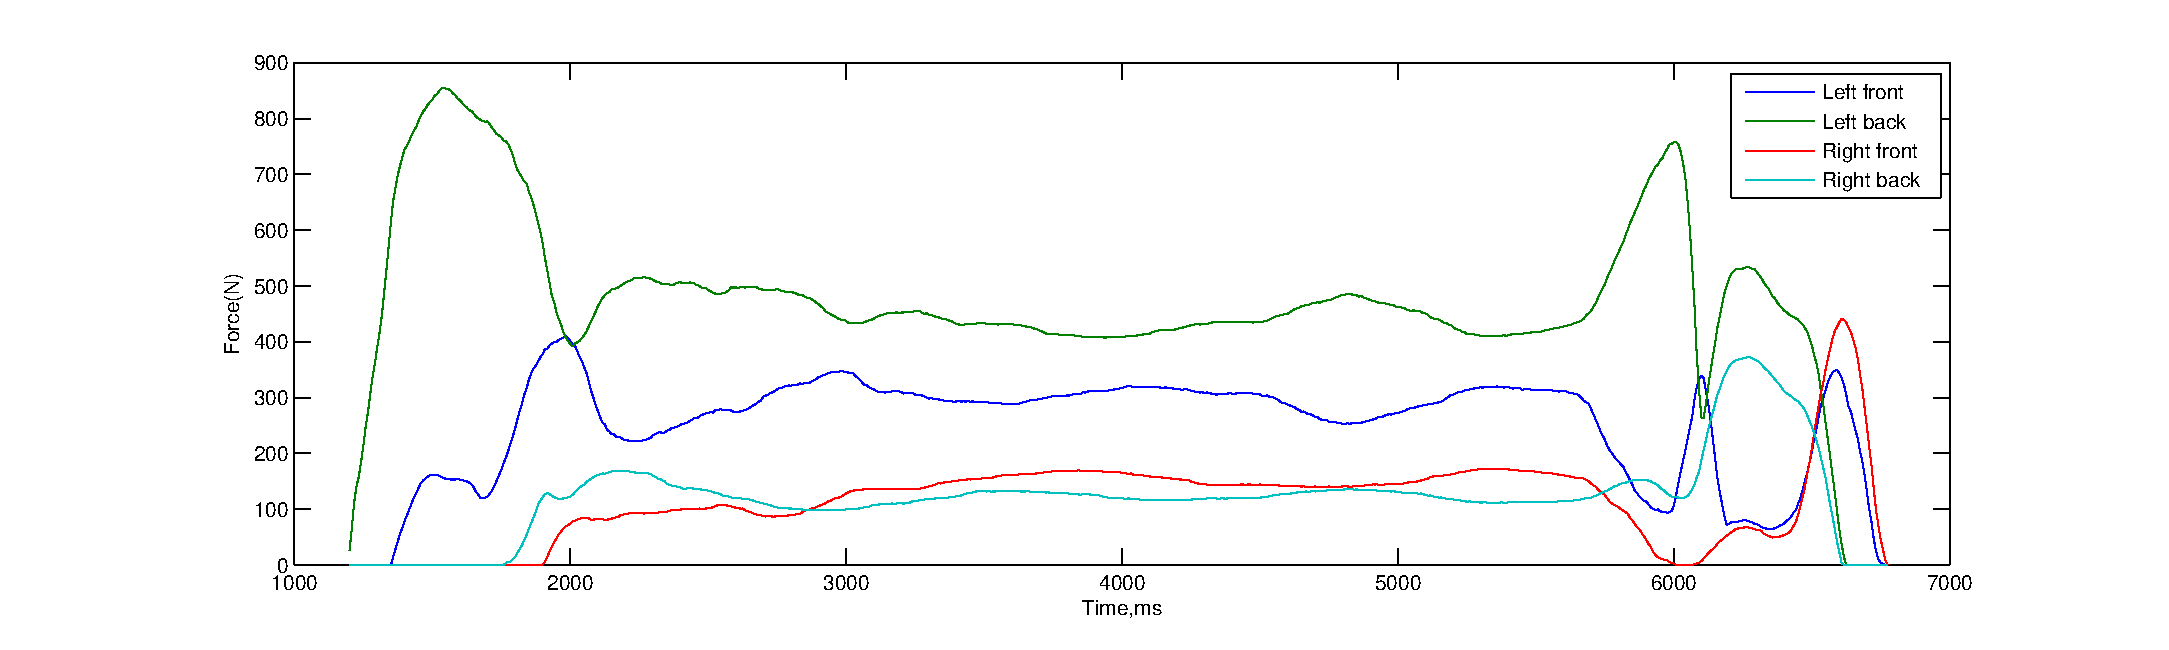
\epsfig{file=figures/Synchronisation/Force4signals, width=1\textwidth}
	\caption{Force in each body segment.}
	\label{fig:Force4signals}
\end{figure}

\begin{figure}[H]
	\centering
	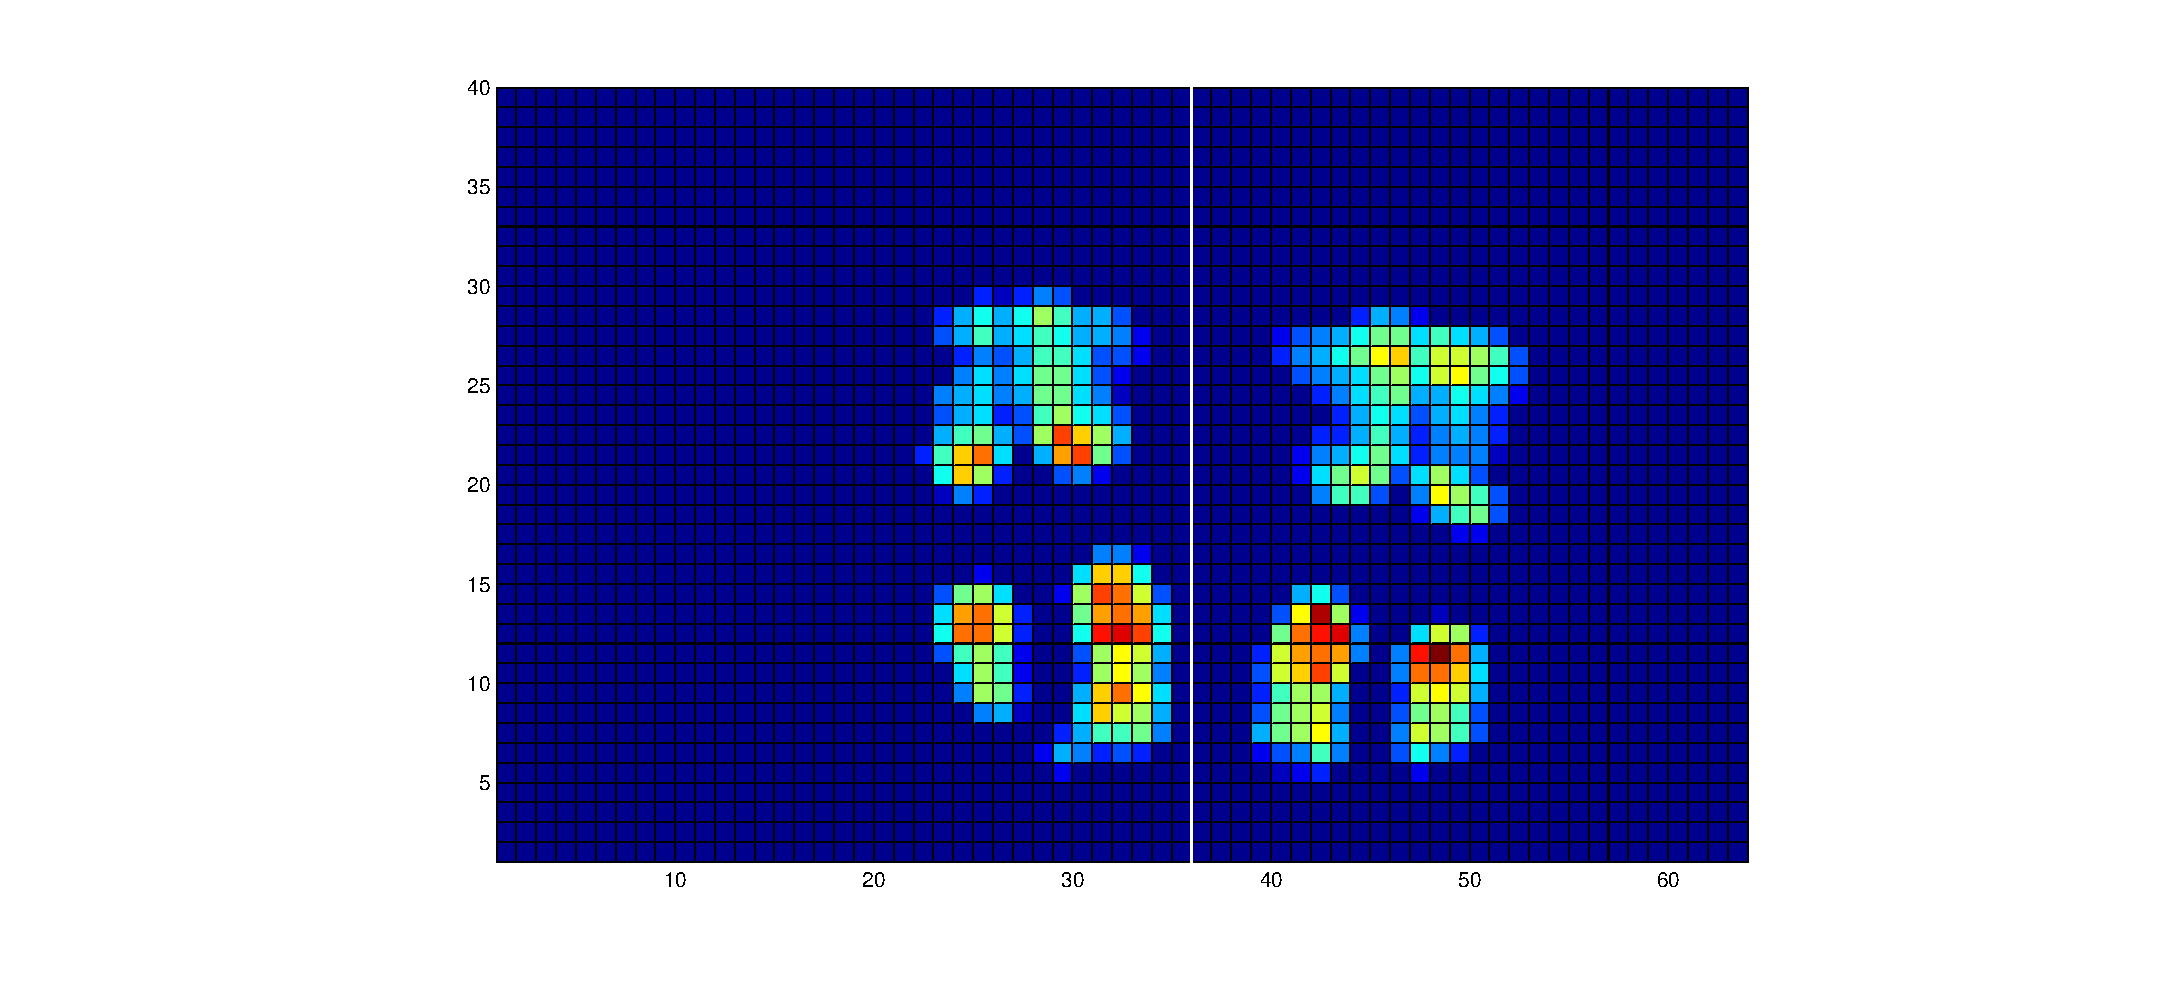
\epsfig{file=figures/Synchronisation/pseudocolor, width=1\textwidth}
	\caption{Pseudocolor with the force in each cell of the platform}
	\label{fig:pseudocolor}
\end{figure}

Once we recover this data, some parameters are calculated for the movement characterization carried out over the platform. 

\begin{itemize}
	\item \textbf{Midline}: it represents the midline between both feet. This is important to find the gap between feet and it gives us a idea of their position in the platform. Thus, we carry out the sum of cells force in the anterior-posterior direction. So, this line is in the minimum between two maximum corresponding to the position of both feet. We use this parameter to calculate the center of pressure.
	\begin{figure}[H]
		\centering
		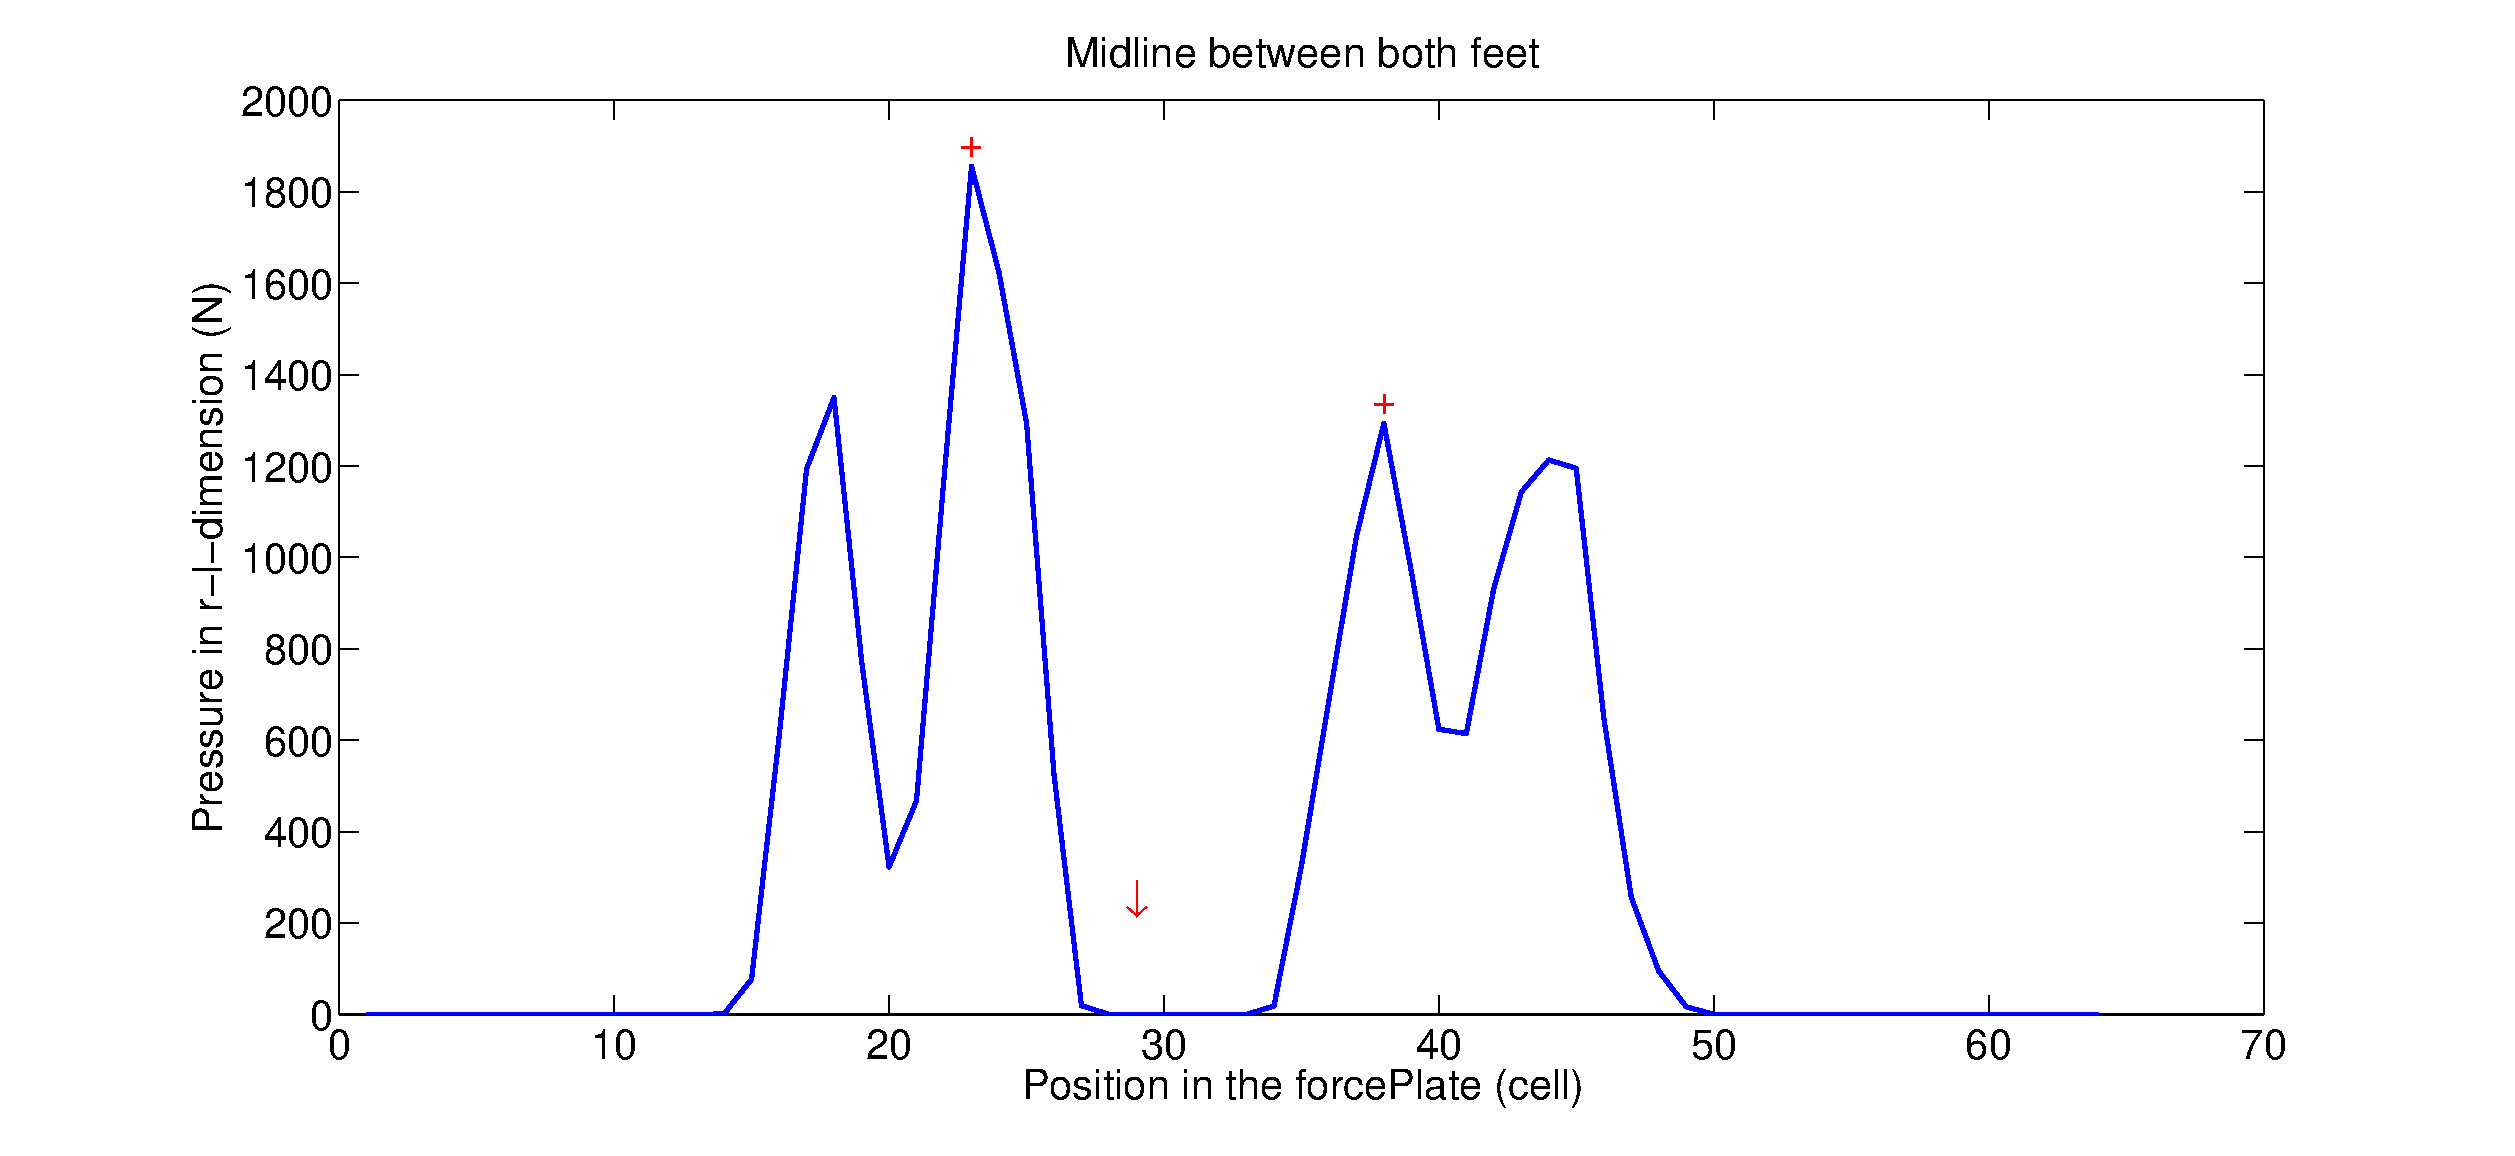
\epsfig{file=figures/Synchronisation/midlineForceplate, width=1\textwidth}
		\caption{Midline between both feet in platform.}
		\label{fig:midlineForceplate}
	\end{figure}
	
	\item \textbf{The total force in the platform for each point of time}: This signal is useful to do the synchronisation due to we can determine clearer when the patient touches the plate.
		\begin{figure}[H]
			\centering
			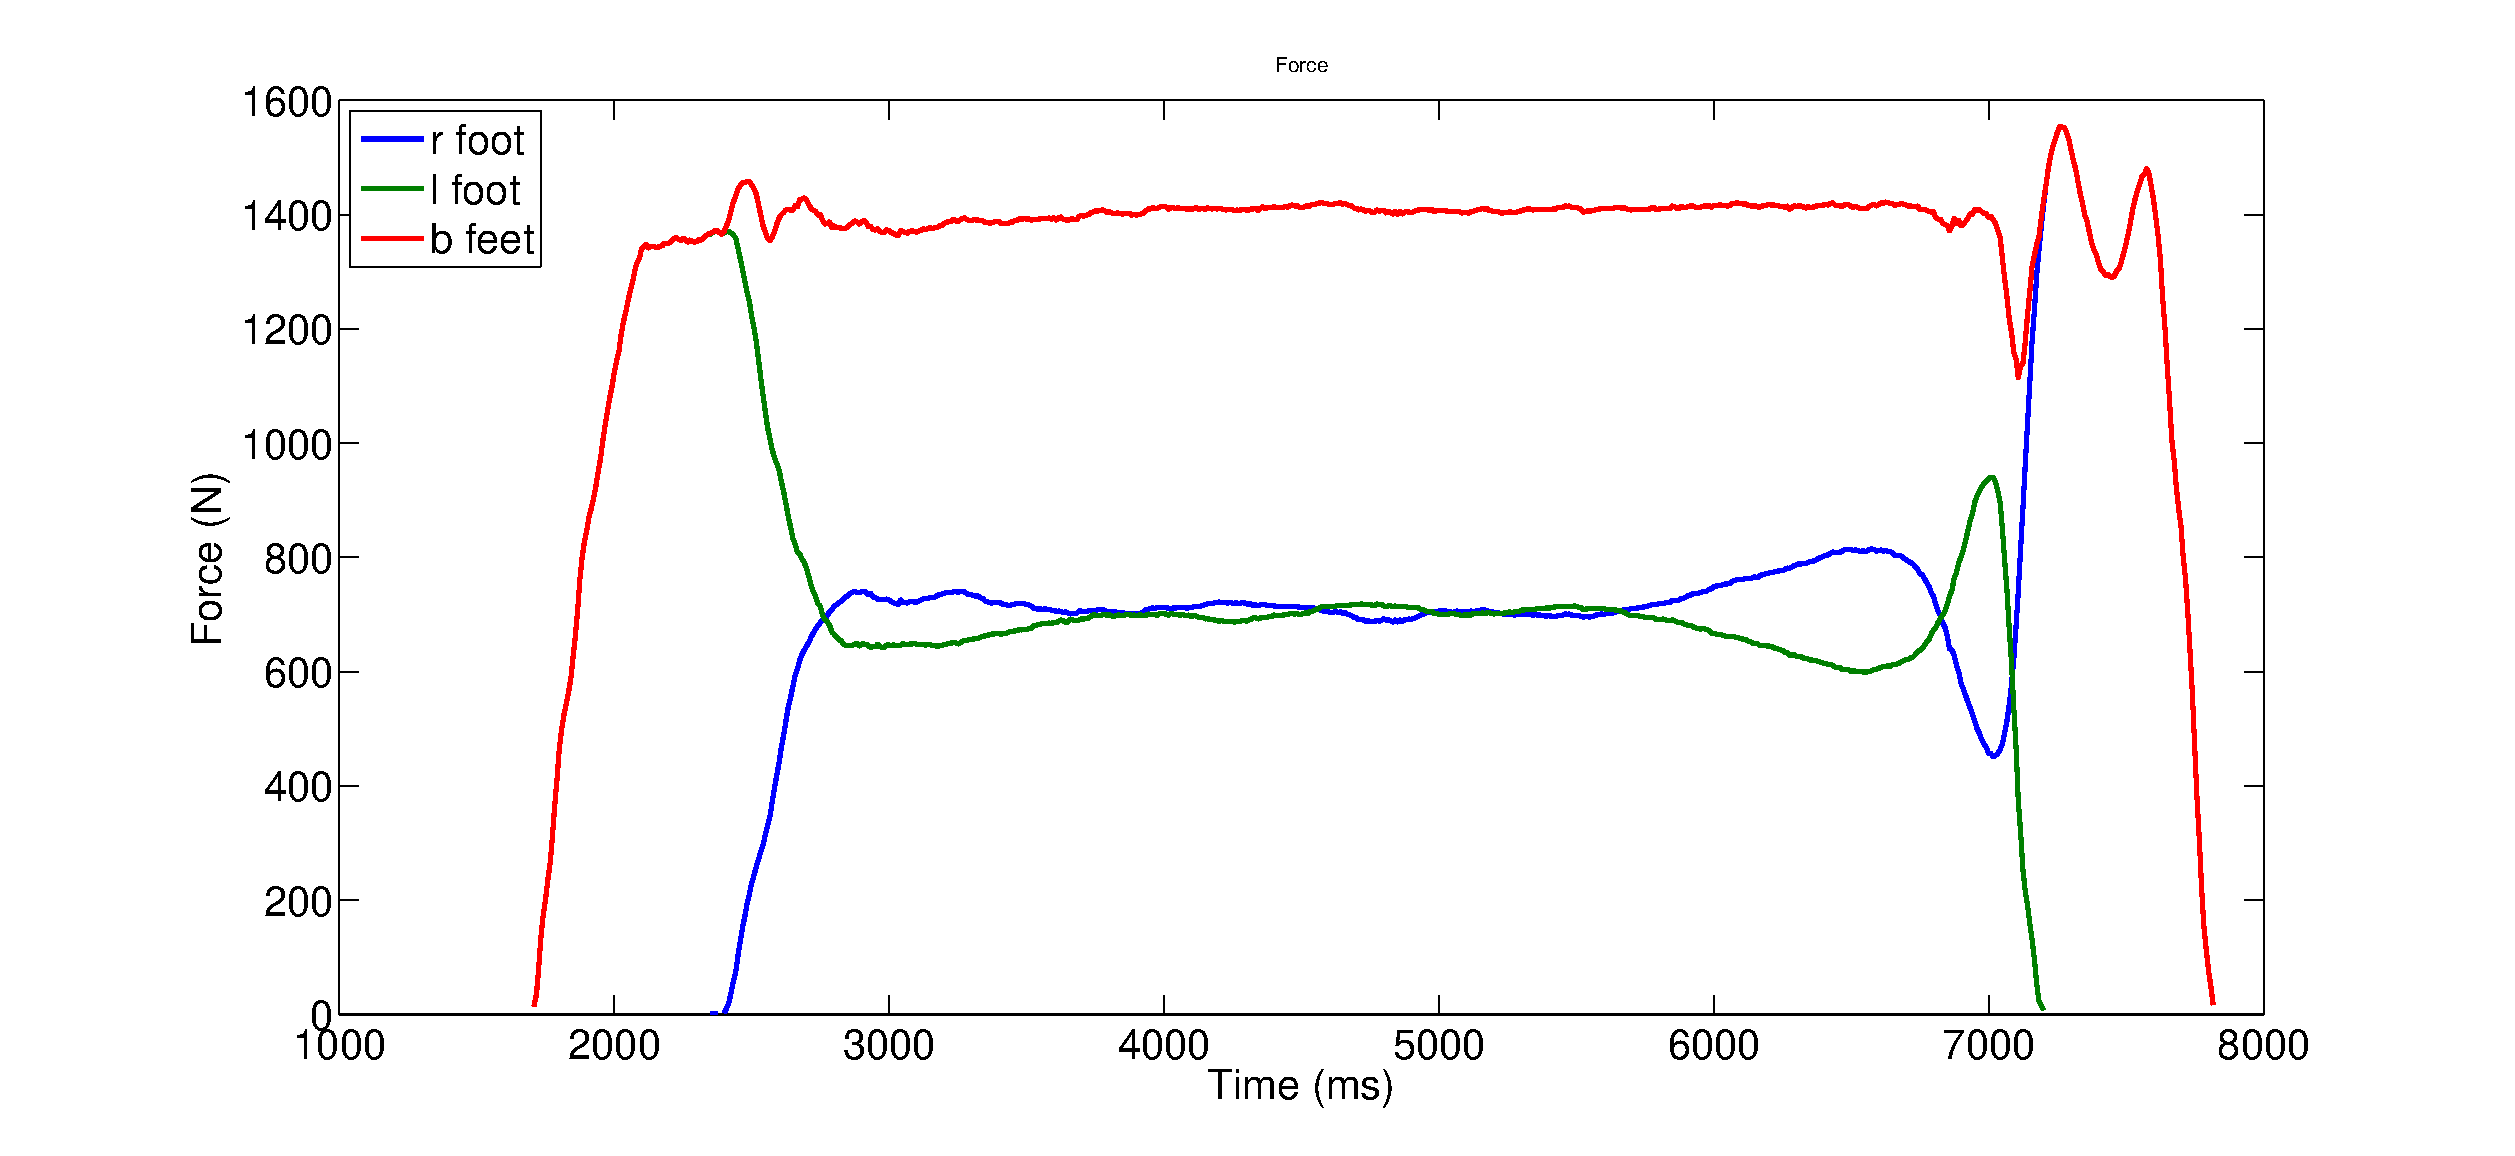
\epsfig{file=figures/Synchronisation/forceFP, width=1\textwidth}
			\caption{Total force in the platform of the right, left and both feet.}
			\label{fig:forceFP}
		\end{figure}
\newpage	
	\item \textbf{Antero-posterior COP}: Center of Pressure in forward-backward direction.
		\begin{figure}[H]
			\centering
			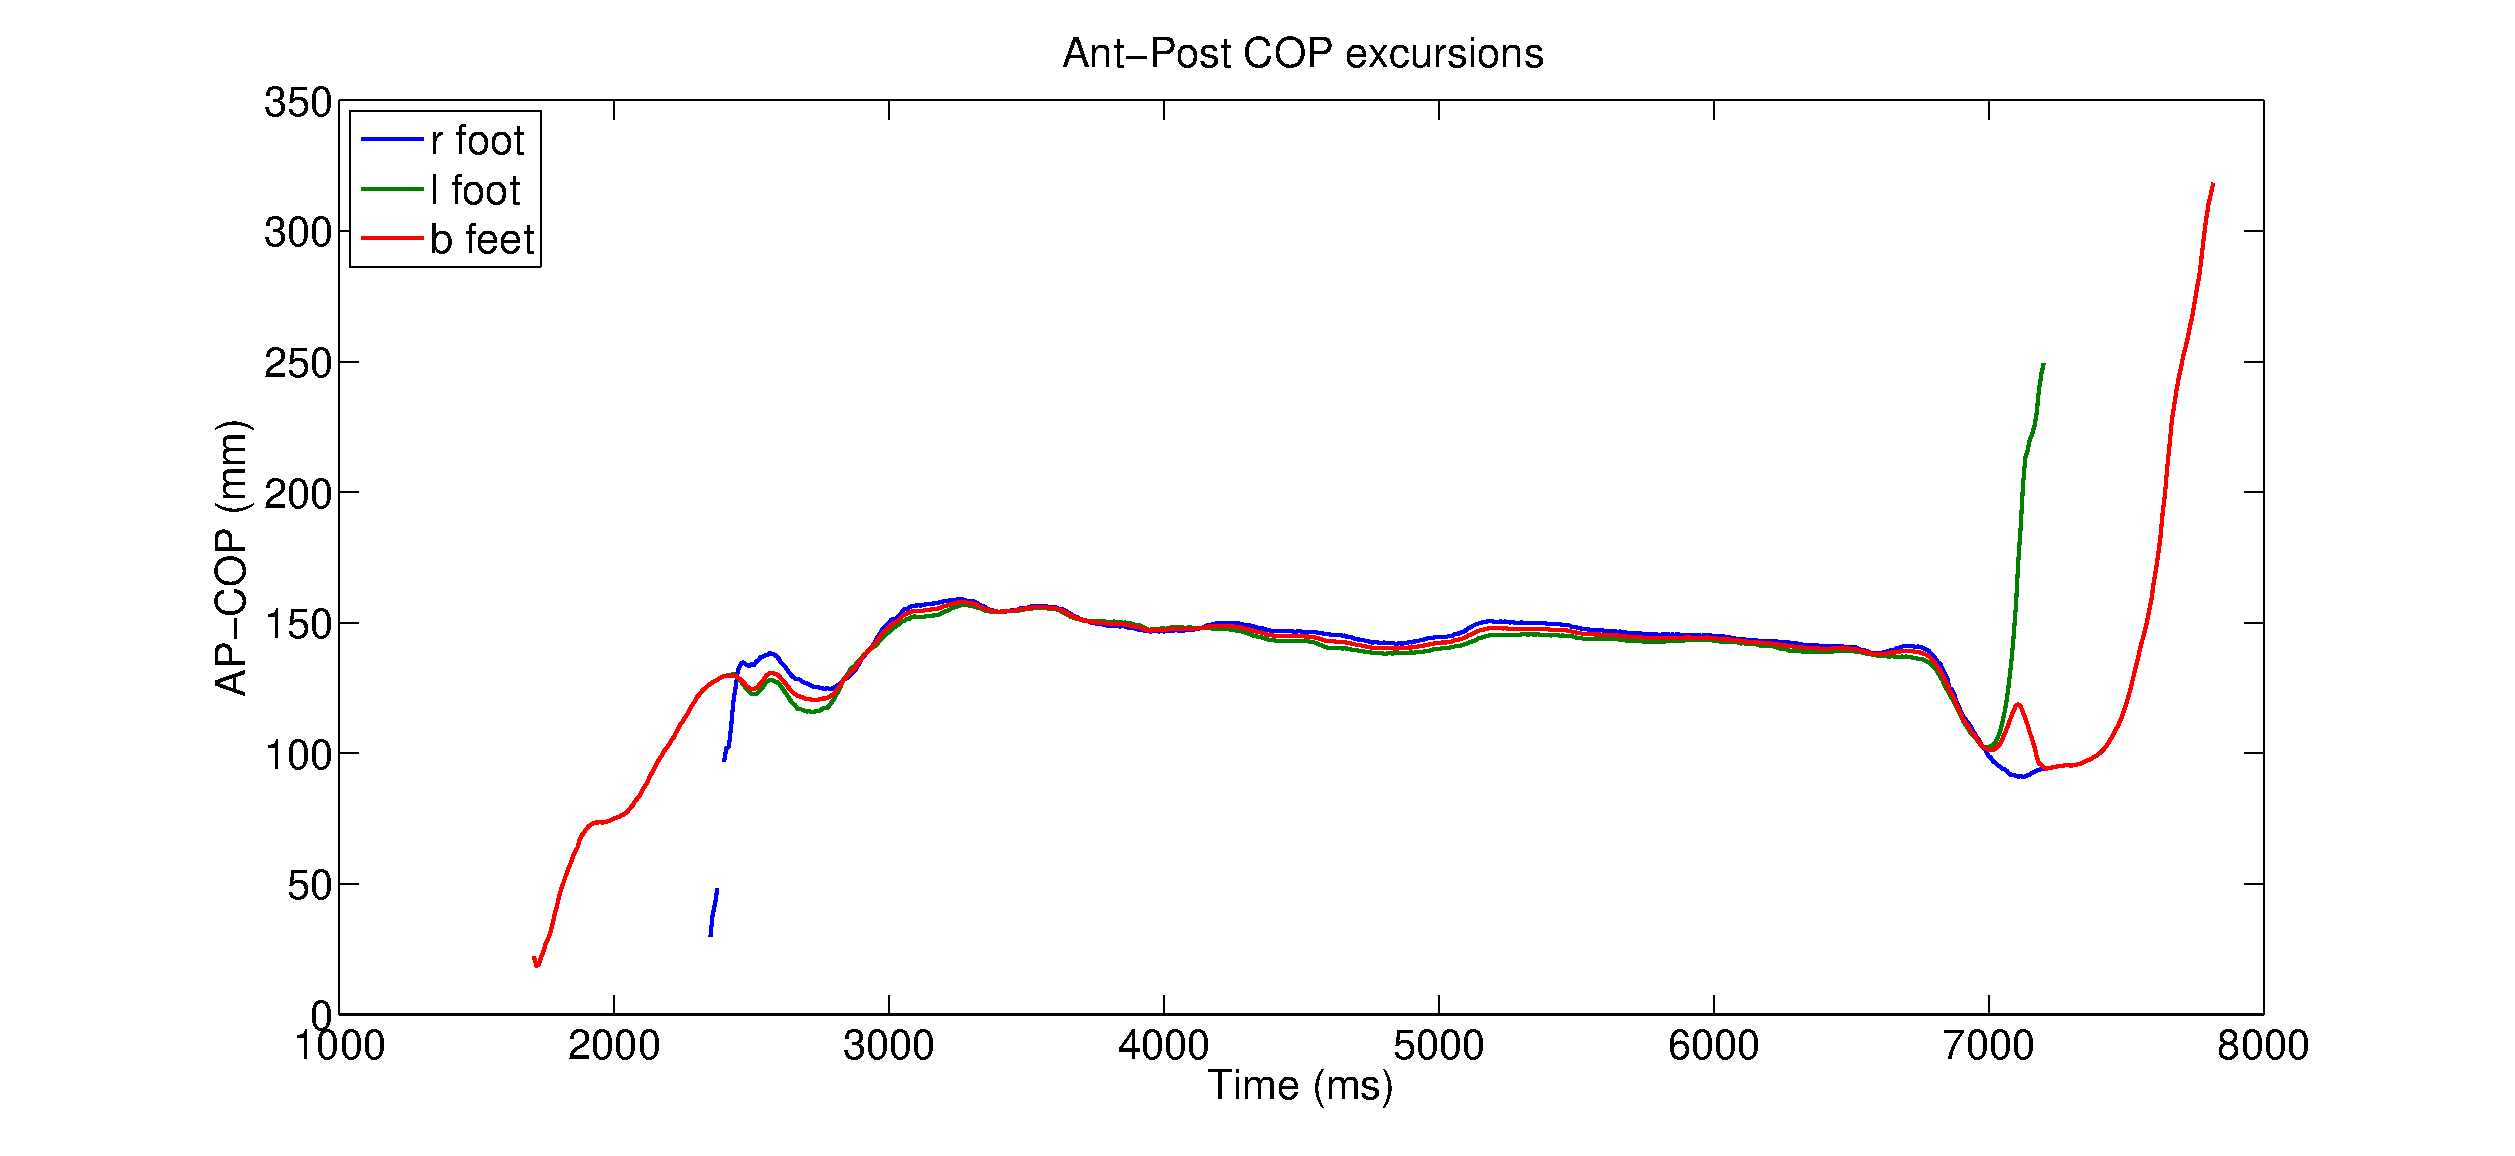
\epsfig{file=figures/Synchronisation/APCOP, width=1\textwidth}
			\caption{Center of Pressure in Antero-Posterior direction.}
			\label{fig:APCOP}
		\end{figure}	
	
	\item \textbf{Medio-lateral  COP}: Center of Pressure  in right and left direction.
			\begin{figure}[H]
				\centering
				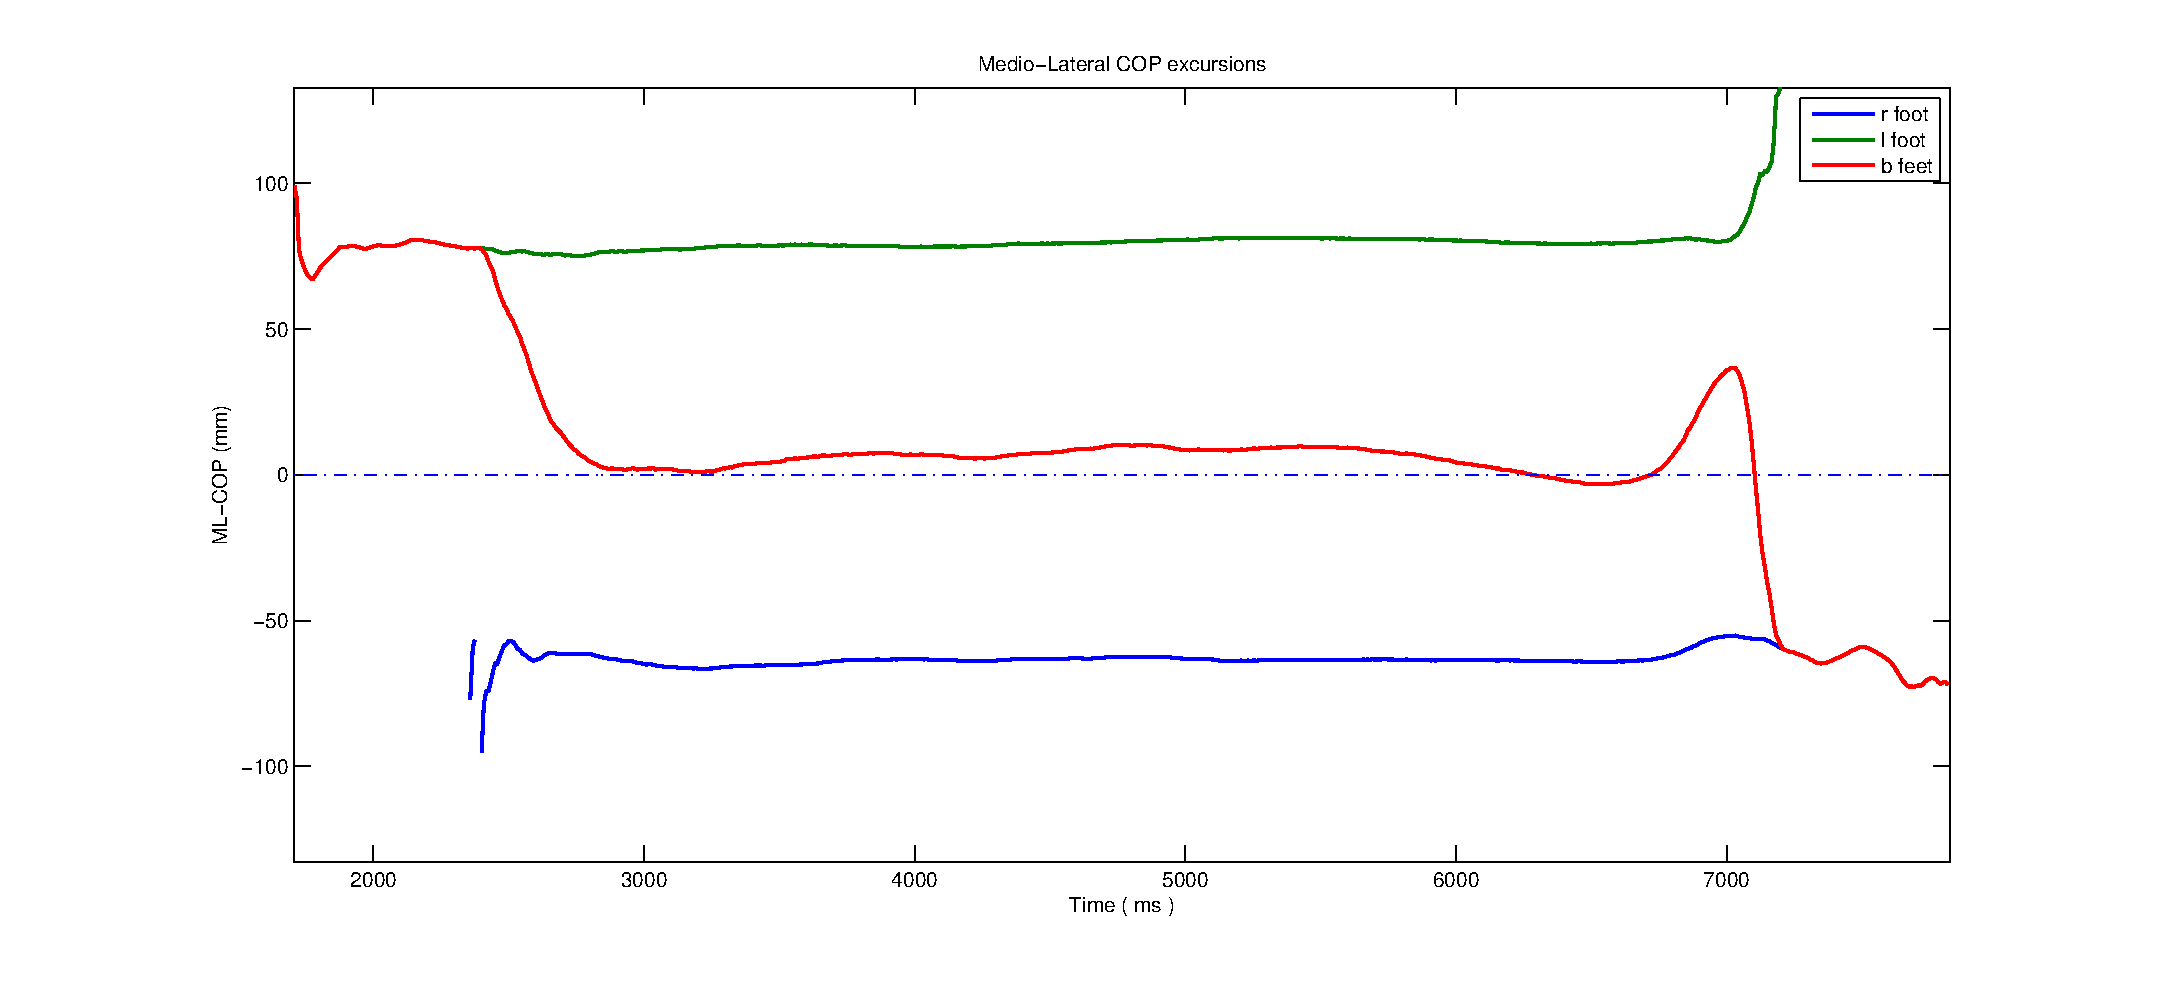
\epsfig{file=figures/Synchronisation/MLCOP, width=1\textwidth}
				\caption{Center of Pressure in Medio-Lateral direction.}
				\label{fig:MLCOP}
			\end{figure}
	
\end{itemize}
\newpage
Center of Pressure can be expressed as follows:

\begin{equation}
	\label{COP}
	R=\sum_{i}^{n}m_{i}r_{i}
\end{equation}


Where \textit{R} is the \textit{“Center of pressure”\textit{}}, \textit{M\textit{}} is the total force and mi are the force that are located in space with coordinated \textit{ri\textit{}}, in this case, in the plane. This location (\textit{ri}) is calculate with respect to the midline.

These signals help us to characterise Anticipatory Postural Adjustments  before gait.  APAs indicate the movement or swinging of body before walk or carry out some movement. Thus, these are the interesting  measures to compare between each repeat as well as each patients to characterise the movement, determine if there is a pattern and figure out the differences and similarities between them.

All these signals are saved for each cycle in a single variable corresponding to the patient.


\subsubsection{Calibration of the GaitWatch data}
When we are working with sensors, calibration is one of the most important aspect that needs to be carried out. Prior to the calibration process,
the information at the sensors  will be a signal composed of integer
numbers  or real numbers bounded into a range which is determined by the precision of the sensors and converters. These numeric values lack of physical value, so it is absolutely necessary to convert them into a scale that can be measured in physical units.

The sensors present several errors due to some effects like scale factor may not be linear or the triad isn’t perfectly orthogonal. To remove these undesired effects, the software include a model to compensate this before the calibration. 
To do so, we have used the code made by Dr. Alberto Olivares Vicente in his doctoral thesis\cite{A.Olivares2013}, with minor modifications of his work.

Besides the unwanted effects mentioned above, the output of magnetometers is distorted by wide band measurement noise appearing several large peaks of noise in the signals. To remove this automatically, we used a threshold considering that these peaks are much greater than the mean of the signal \ref{fig:GWErrorDetected}.

The erroneus values in the magnetometer signal are removed sustituting these samples by the subsequent value unless the erroneous value is in the last position of the singal, in which case it is substituted by the preceding value.

\begin{figure}[H]
	\centering
	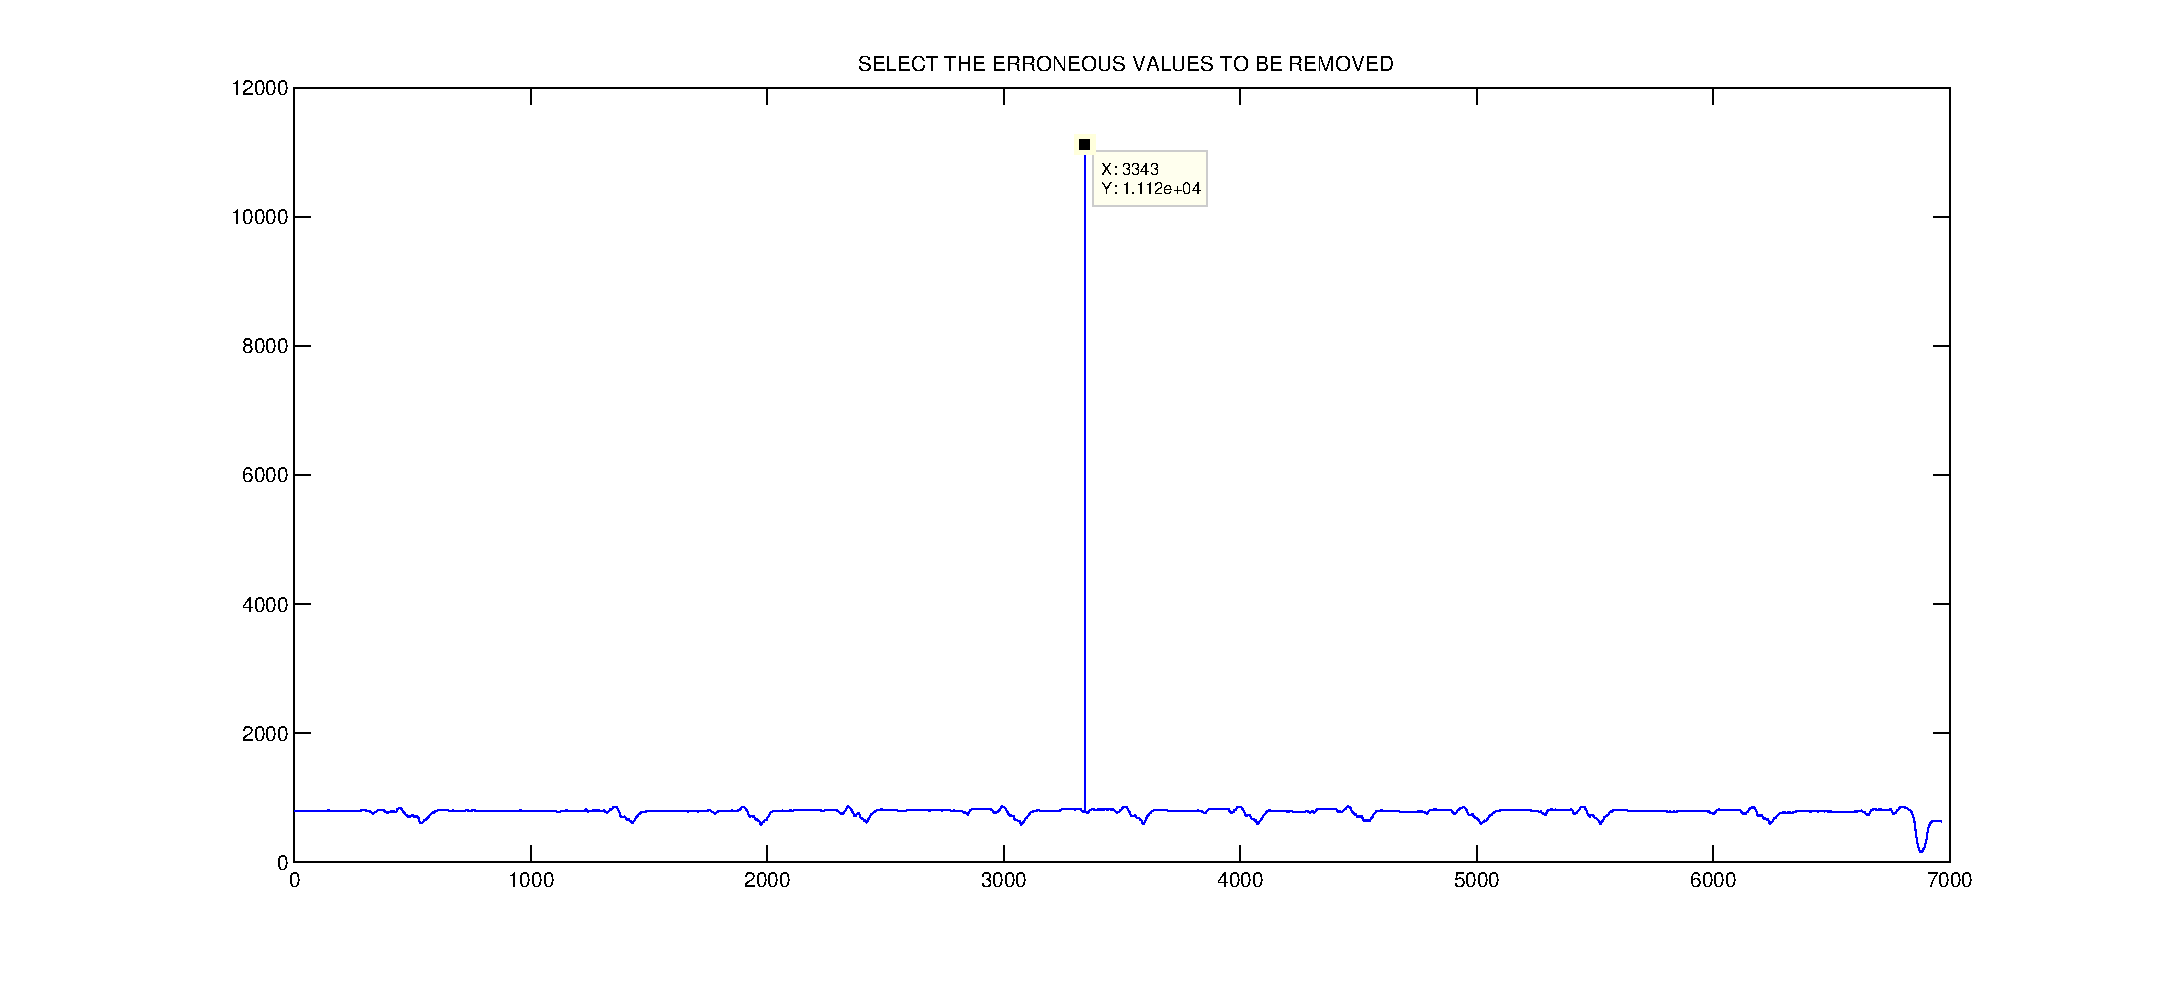
\epsfig{file=figures/Synchronisation/GWDetectErrorValueAutomatically, width=18cm}
	\caption{Value erroneous in magnetometer signal detected automatically.}
	\label{fig:GWErrorDetected}
	\end{figure}



\subsubsection{Synchronisation}	
In this section we will explain how we carried through the synchronisation of the Force Plate and GaitWatch signals and the considerations adopted to do it properly.

The first step is to detect when the step happens in both systems. In order to do this, we’ll use the completed force from Force Plate system and shank acceleration from the Gait Watch accelerometer. We chose these signals because it is easy to see in them the point when the patients step.

Once we have selected the right signals to do the synchronisation we have to differentiate each cycles in the acceleration signal because we have all repeats together in the same file. To do this, we used activity detection code implemented by Dr. Alberto Olivares Vicente in his Doctoral thesis. Figure \ref{fig:activityDetection} shows the result.

In addition we did a comparative study testing two different methods based on the  computation of the spectrum (Fourier Transform) of the input signal. Also, we tried several input signal to determine which is the best option to do the motion detection in this case.

We will use the Long Term Spectral Detector (LTSD) \cite{Ramirez2004} and a variation of this called Framed Spectrum Detector (FSD). Spectrum-based methods have been used in others kinds of applications like Voice Activity detection \cite{Ramirez2006}\cite{Ramirez2007} and activity sequences detection such as running or sitting-standing up\cite{A.Olivares2013} .

The technical difference between LTSD and FSD is that the first of them compute the Long term spectral Envelope whereas FSD uses the spectrum of each frame  in which the input signal is divided\cite{A.Olivares2013}. What we observe when we use them in our signals is that the results are better when we use LTSD instead of FSD method  in the most of the cases\ref{fig:activityDetection}.

\begin{figure}[H]
	\centering
	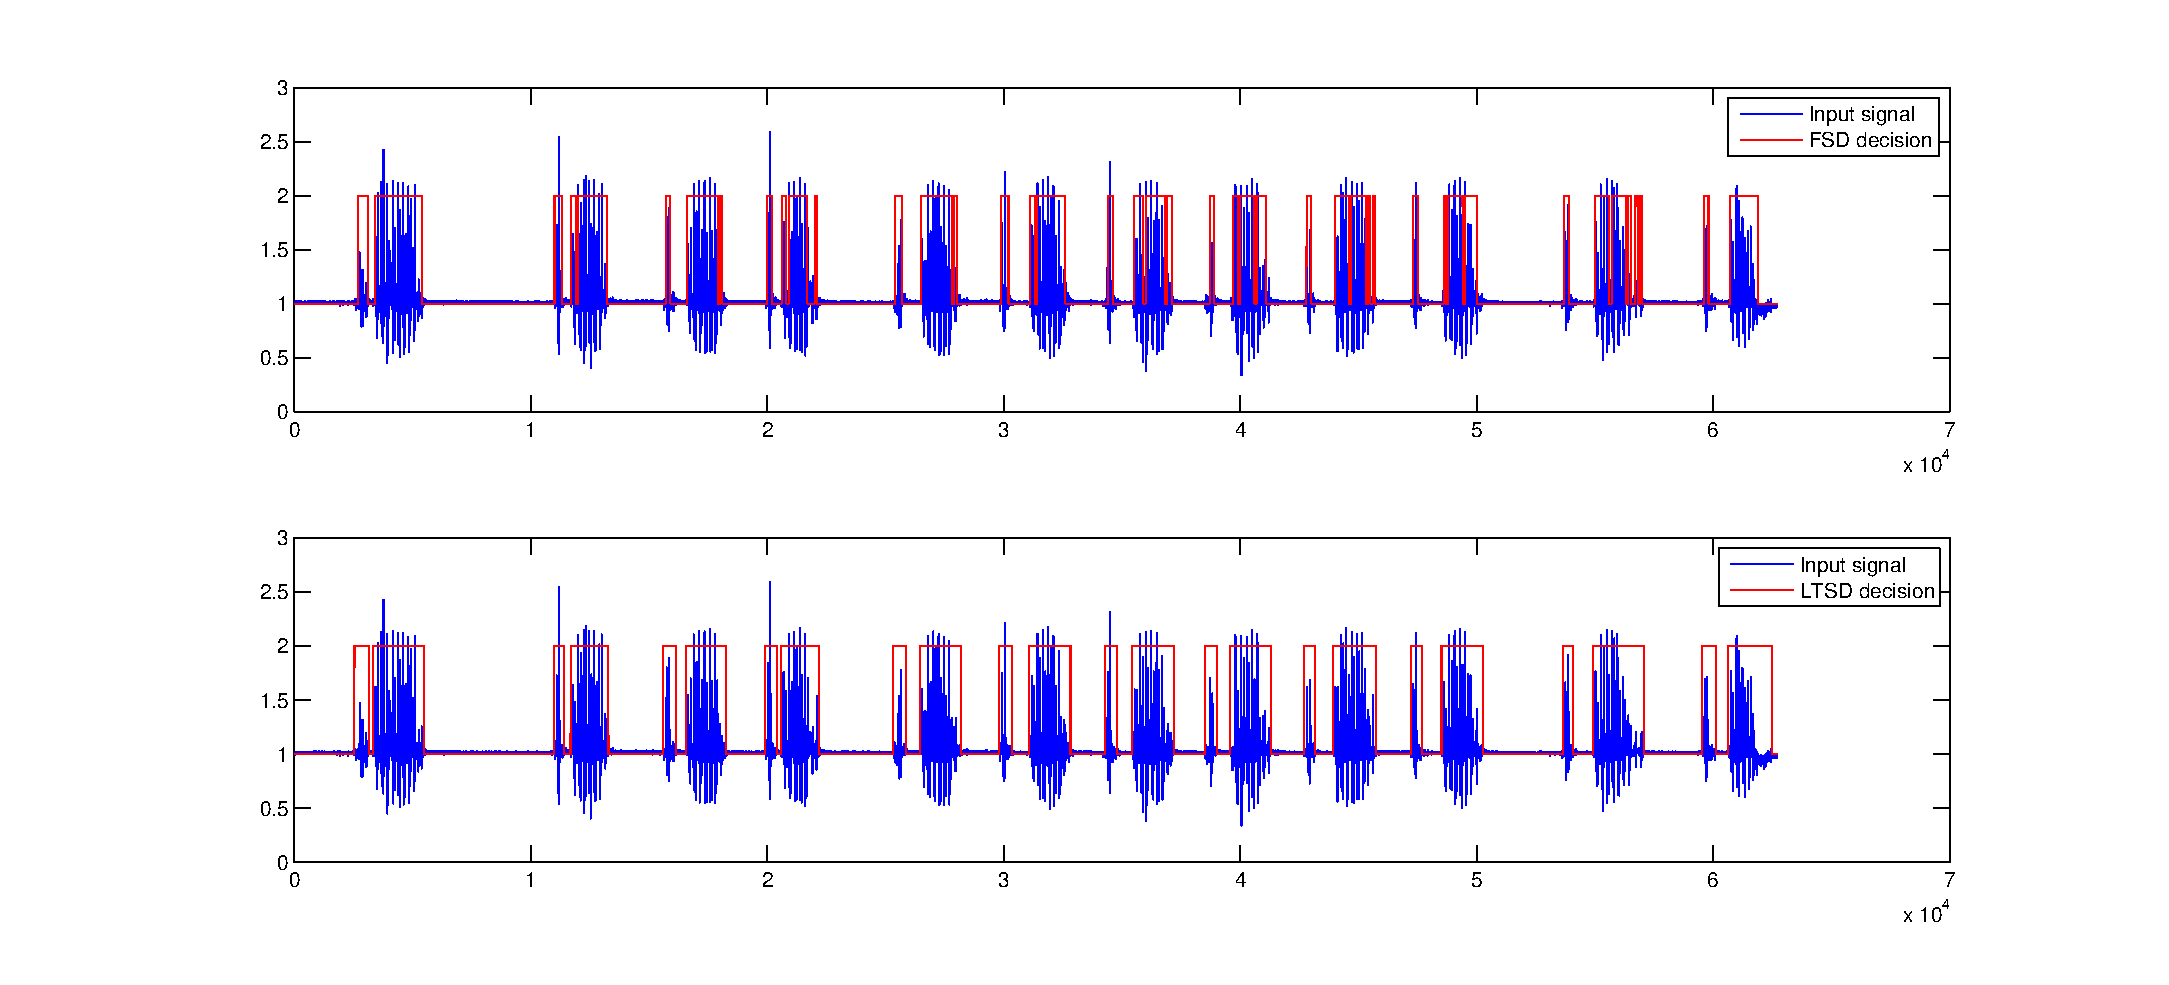
\epsfig{file=figures/Synchronisation/activityDetection, width=1\textwidth}
	\caption{Activity Detection with FSD and LTSD Algorithm.}
	\label{fig:activityDetection}
\end{figure} 

The LTSD method has a better decision rate than FSD method because it is designed to work under condition where the SNR is low, i.e the signal present large noise\cite{A.Olivares2013}. In our case, we want detect the differents cycles that corresponding to each repeat so the different peaks of activity inside each period can be a problem to do the detection correctly because really it is interpreted like noise for the detector. Thus, the LTSD method is more interesting for this type of signal.

Once we select the best method for detection we tested several input signal for the detector: shank acceleration signal, absolute value of the shank acceleration signal and module of the shank acceleration signal. Finally, the best result was obtained when we used module of the shank acceleration signal because when this input signal is used in the resulting output signal is easier to distinguish the different episodes.

Furthermore, the motion activity detection was carried out for the right leg as well as left one. It is not necessary in some cases when the patient does the movements or activities quickly since the detected activity interval  include both movements in the same episode. However, when patient waits some time to step again in the same repeat, it is possible that some step is not  include in the interval thus the result would be erroneous. Therefore, to realise a general algorithm useful in whatever case we differentiate between both feet.

Once the cycles have been separated, we are going to detect the key points in the signals to do the synchronisation. 

On the one hand, the time point when the patient does the step in the platform is exactly when the person touches it, that is, the time point that corresponding with the first sample in the force signal with a value other than zero.

\begin{figure}[H]
	\centering
	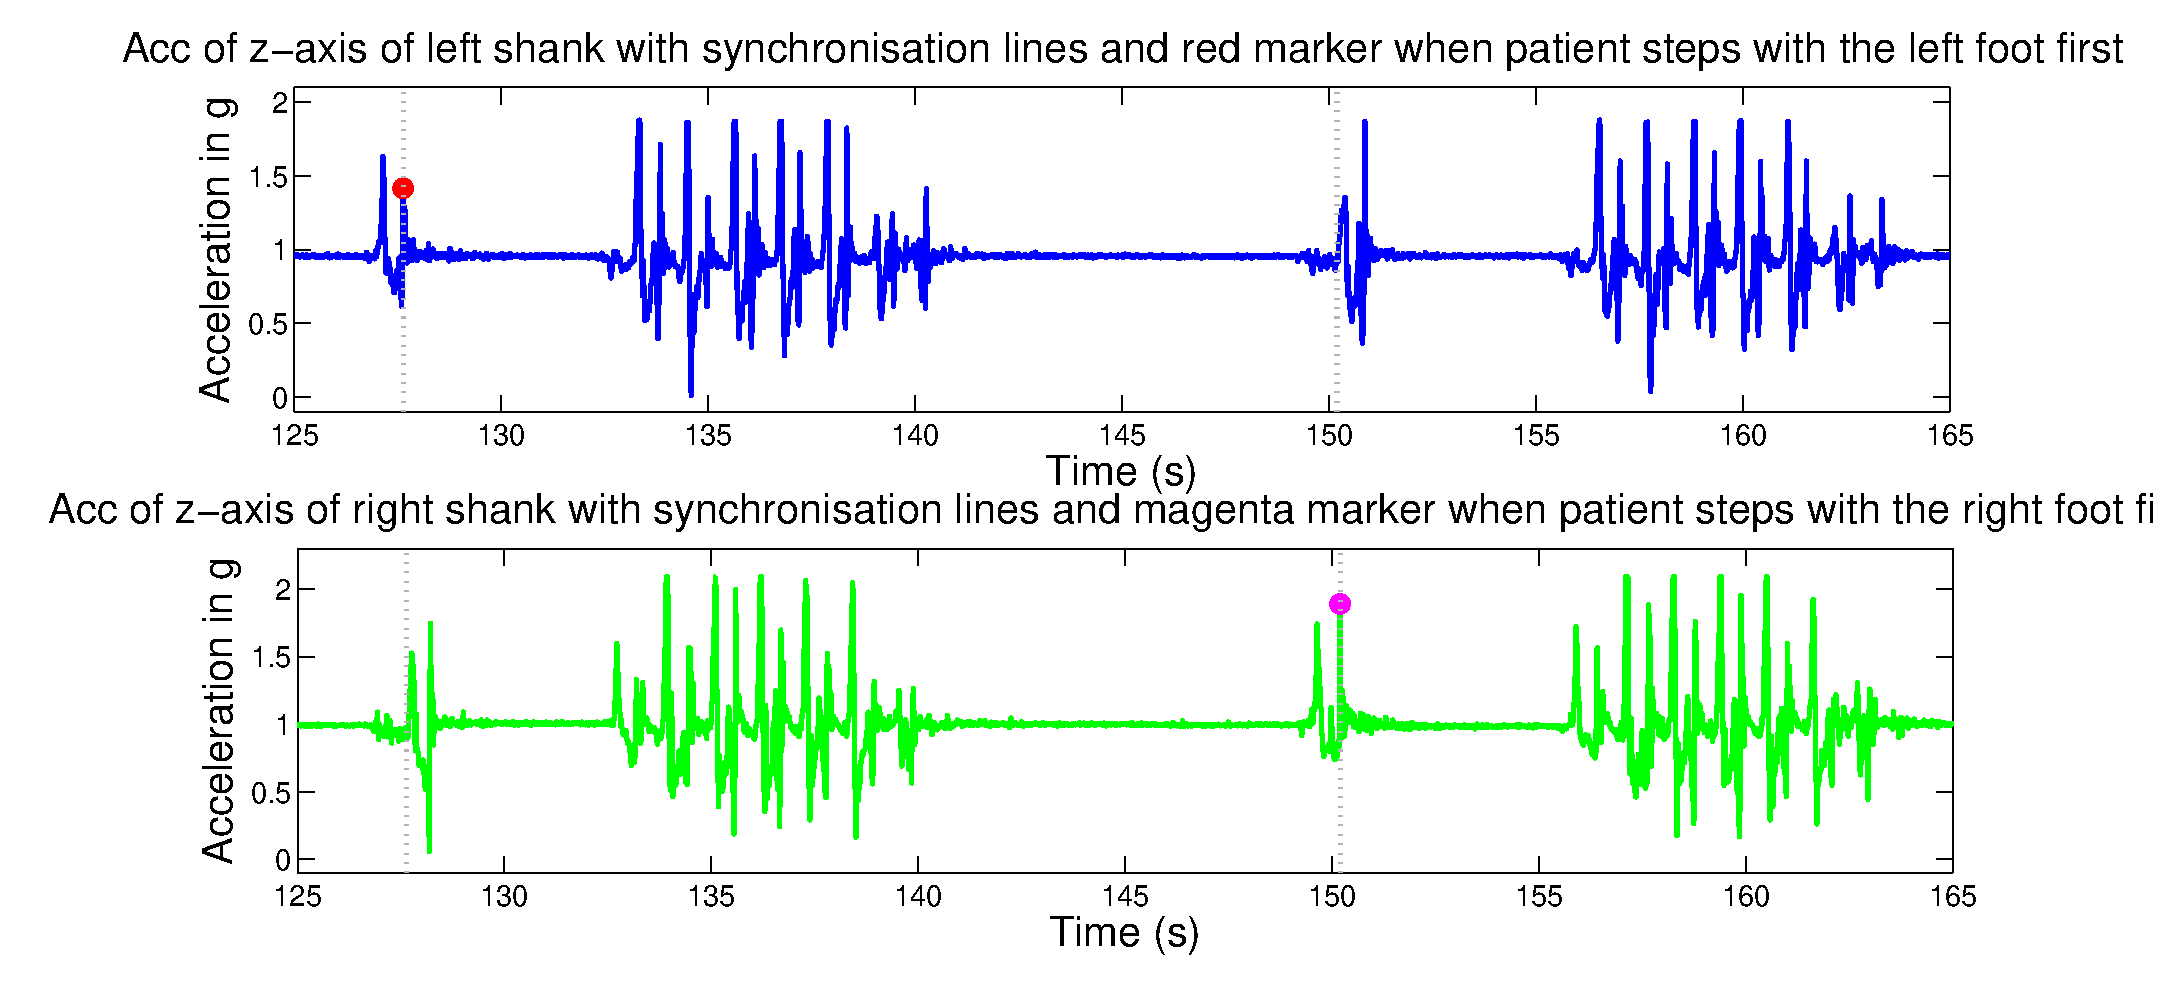
\epsfig{file=figures/Synchronisation/startLeftRight, width=1\textwidth}
	\caption{Accelerometer signals when the patient starts to step with the left and right foot respectively.}
	\label{fig:startLeftRight}
\end{figure} 

On the other hand, in the acceleration signal case, this fact happens in the second positive peak\ref{fig:pointdetectionAcc}. The reason is that when patient does a step, the first movement is to rise the leg, so the acceleration vector points upwards thus the great positive peak will be when the leg is in the maximum distance from ground. Then, there is a change of direction and it appears a negative peak in this trace. The immediate movement is to lower the leg and touch the platform, so when the patient puts his leg in the force plate there is a positive peak due to the acceleration vector is pointing upward again.\ref{fig:sinchronisedSignals}.

Now, we have to consider others aspects like the limbs with which the person start to walk. To do all more comfortable for the patients, it was not specified with which leg they had to do the first step, so we have to determinate automatically this fact. To realise this we calculate all interesting peaks in the right shank acceleration as well as left shank acceleration. Then, we identify first peak in time \ref{fig:startLeftRight}.

Other important aspect is to consider the sample frequency. The sample frequency is 120 Hz in force plate signals and 200 Hz in GaitWatch signals. Thus, we have to reshape the Force Plate signals to match other signals.

All the key parameters and signals are saved using “time series”  for adding descriptive information to the fact.

\begin{figure}[H]
	\centering
	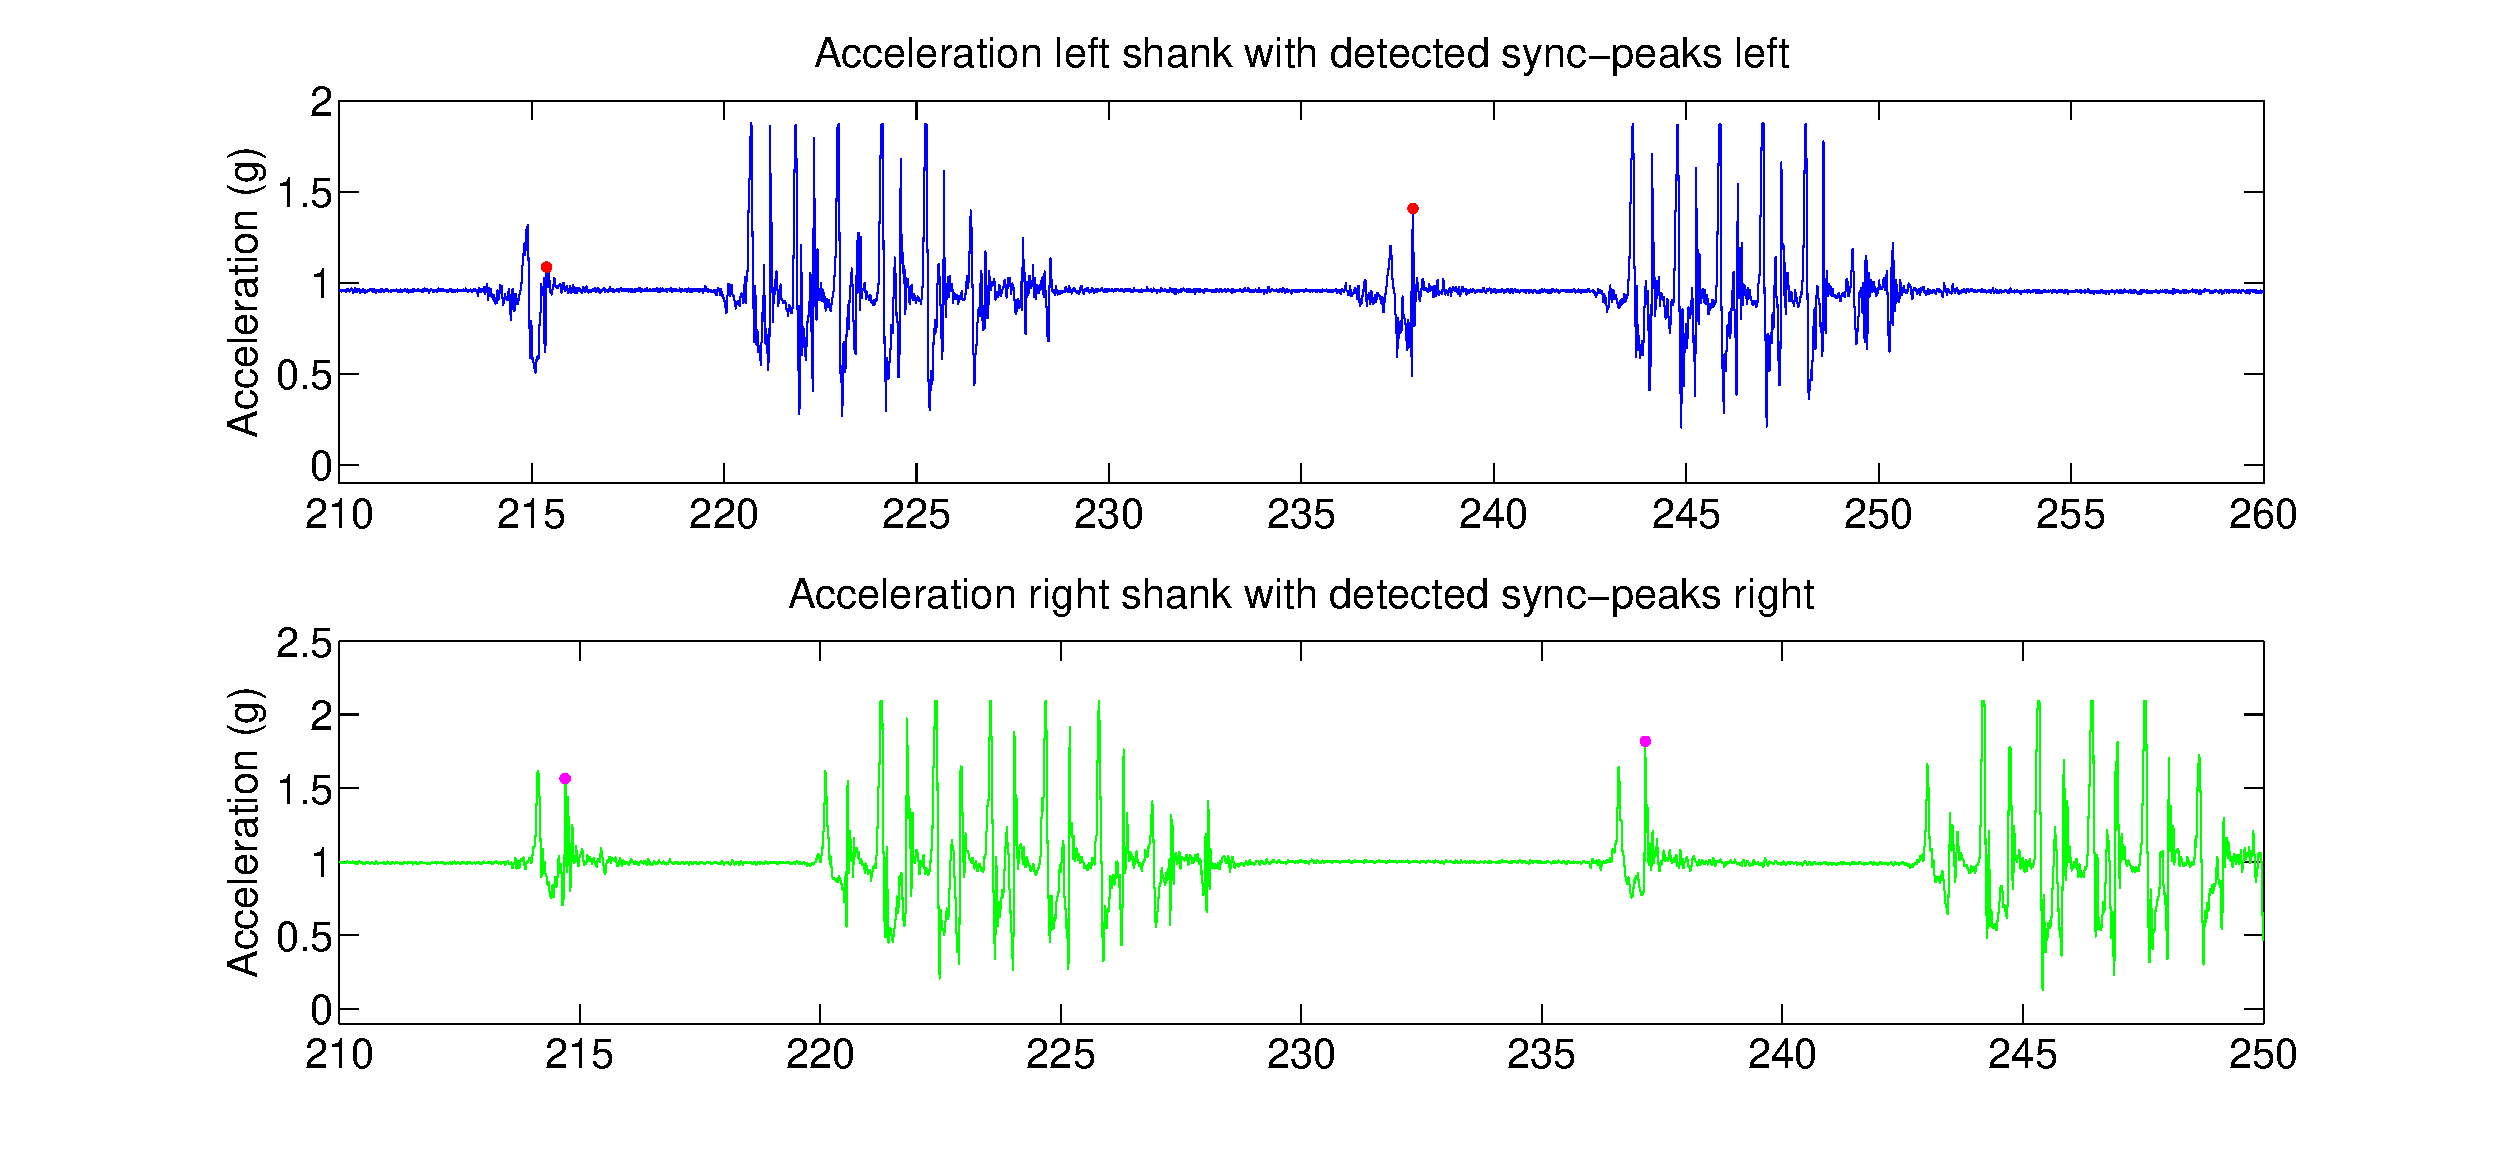
\epsfig{file=figures/Synchronisation/pointdetectionsynchronisation, width=1\textwidth}
	\caption{Peaks detected for the Synchronisation in the Accelerometer signals.}
	\label{fig:pointdetectionAcc}
\end{figure}

\begin{figure}[H]
	\centering
	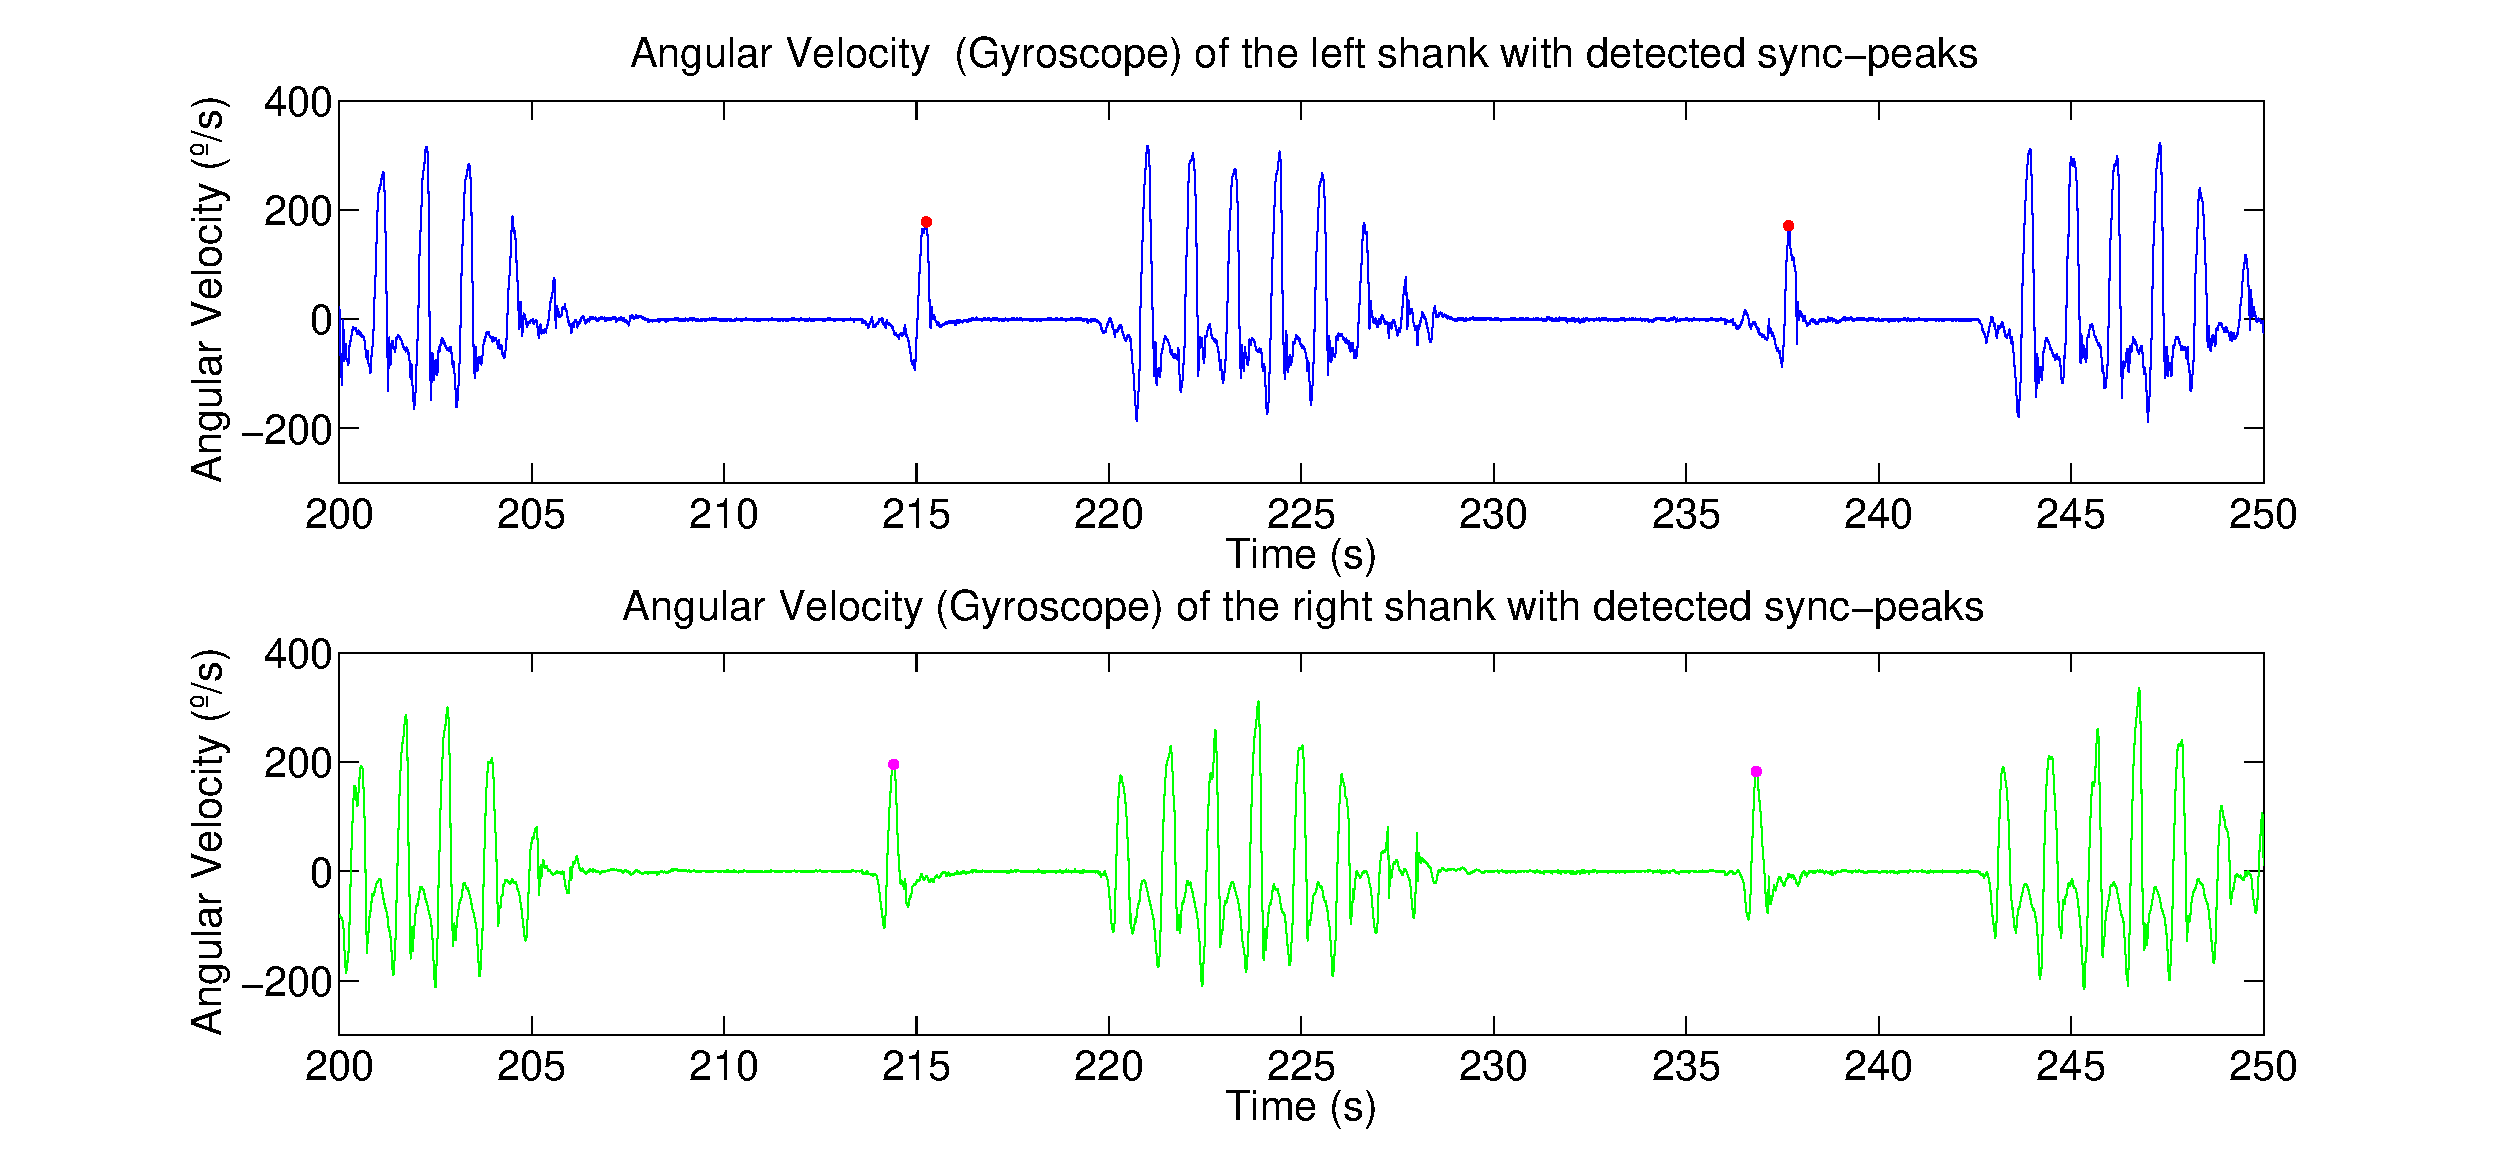
\epsfig{file=figures/Synchronisation/gyrosPointDetection,  width=1\textwidth}
	\caption{Peaks detected for the Synchronisation in the Gyroscope signals.}
	\label{fig:pointdetectionGyro}
\end{figure}

Finally, we compare the peak detection for the synchronisation between the accelerometers signal and the gyroscopes signal. The behaviour of the gyroscope signal is clearer to the naked eye. We can sense there is a negative peak when the patient raises his leg to step. This is negative because the movement is upwards and the Z axes is pointing to the floor so the Angular Velocity is negative. The next positive peak of happends when the person touches the platform so this is the key point to use in the synchronisation\ref{fig:pointdetectionGyro}.

If we compare the behaviour of both signal, it makes sense because a peak of acceleration have to appear when there is a strong growth (or decrement) of the velocity, and this happends when the person go up or down the limbs\ref{fig:pointdetectionAcc}\ref{fig:pointdetectionGyro}.

The correlation between the peaks detected with both systems is very high and the difference between the locations of the peaks are very small as well. This indicates that it was done correctly and these detected points are suitable to do the synchronisation. We can see this in the folllowing figures:

\begin{figure}[H]
	\centering
	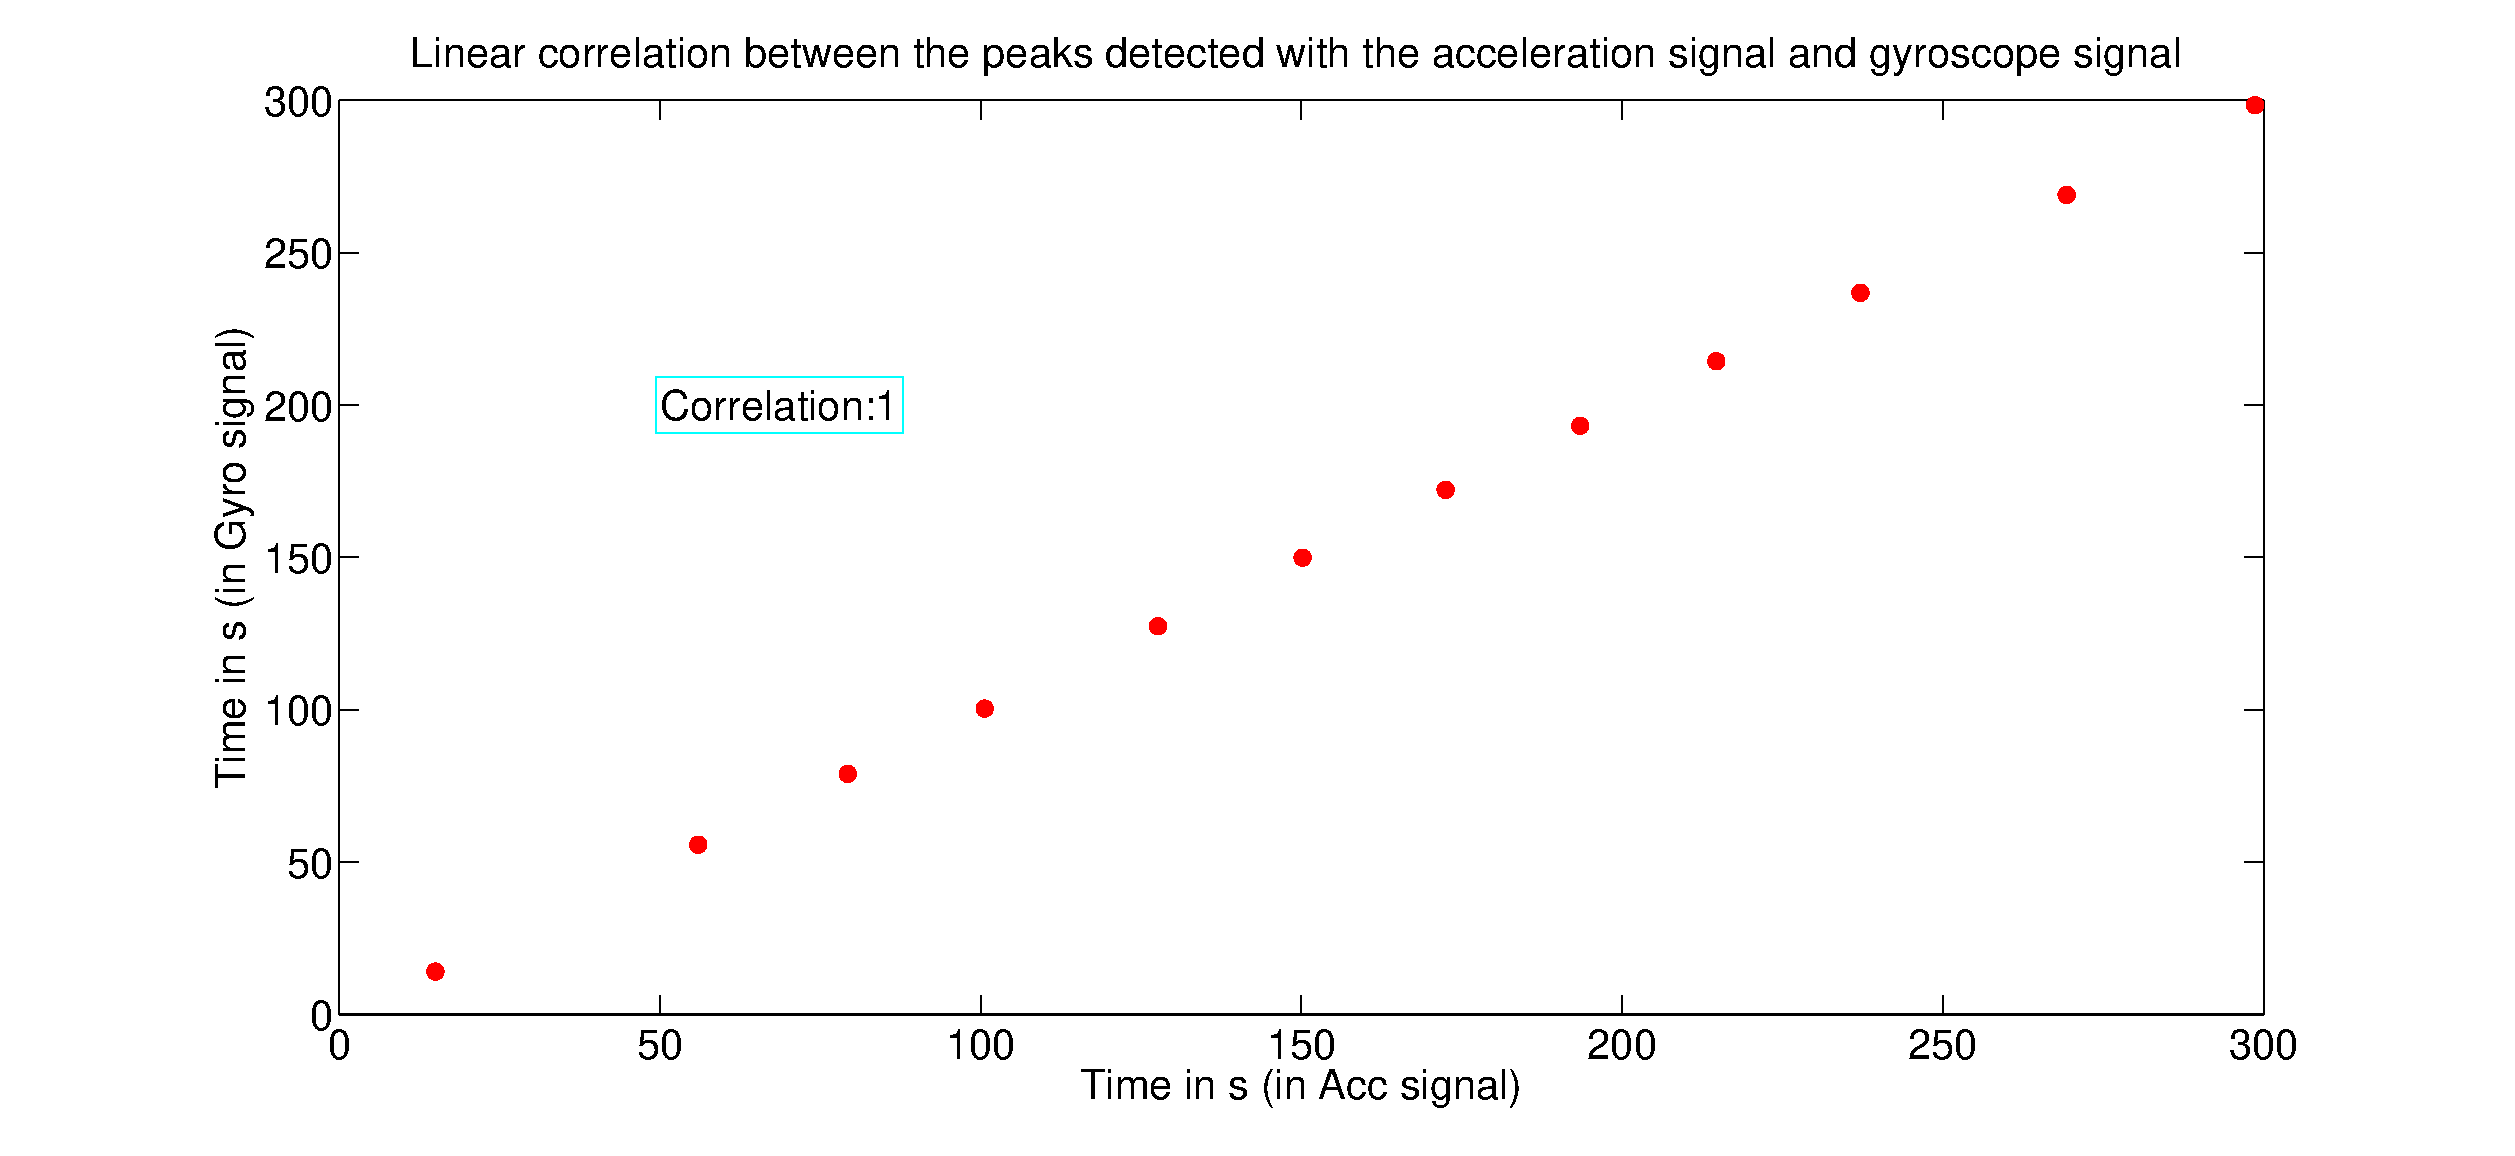
\epsfig{file=figures/Synchronisation/corrAccGyroPoints, width=0.9\textwidth}
	\caption{Linear Correlation between peak Acc and peak Gyro used for the synchronisation.}
	\label{fig:corrAccGyroPoints}
\end{figure}

\begin{figure}[H]
	\centering
	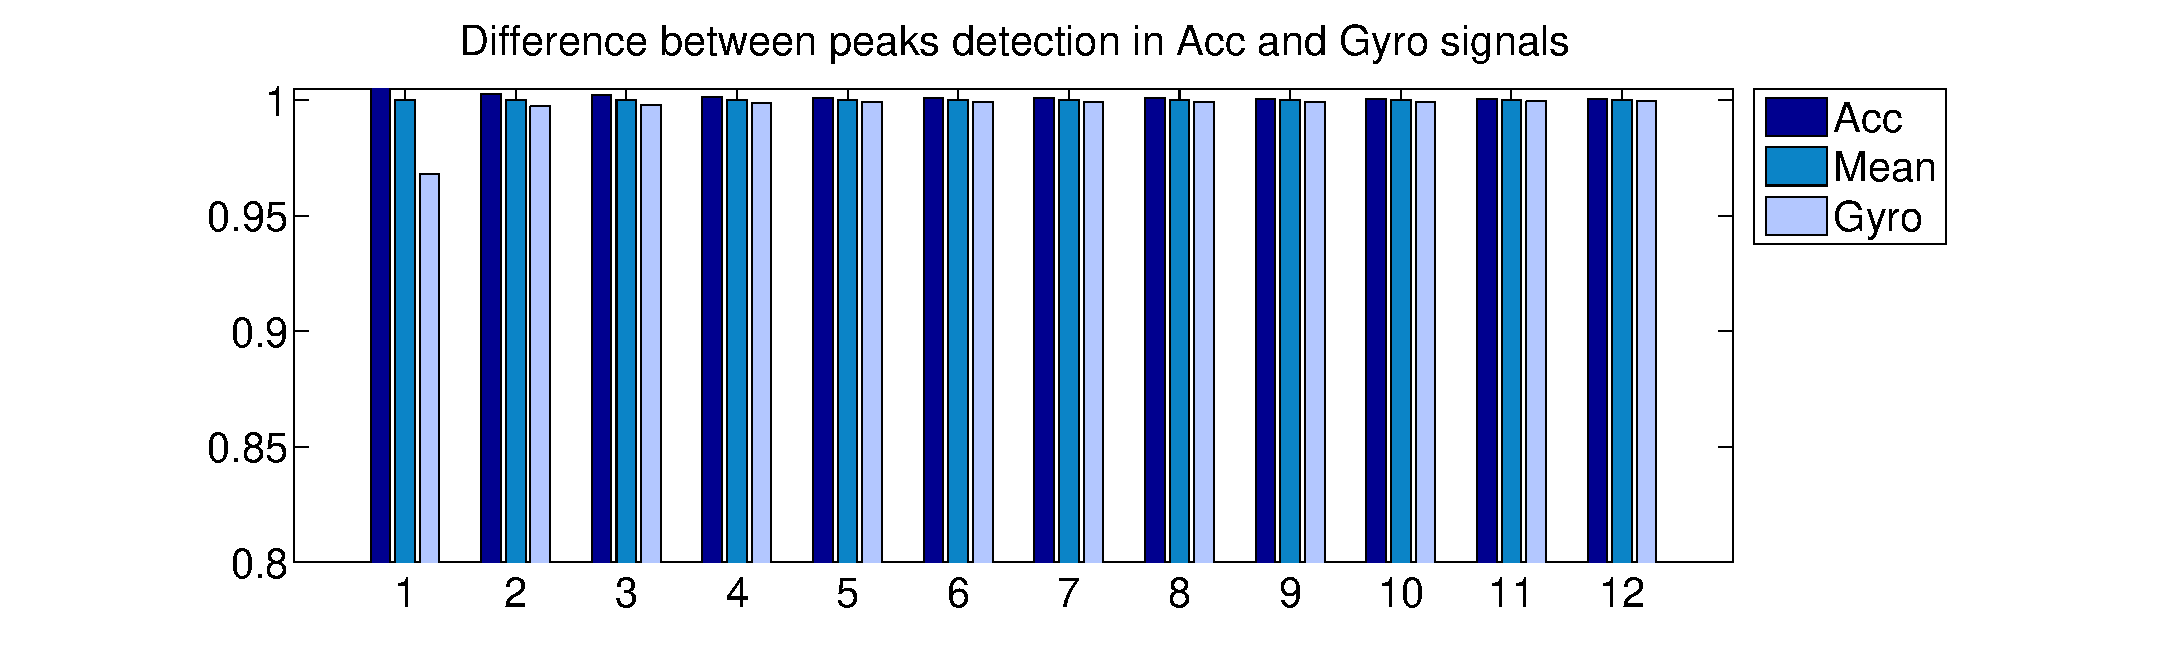
\epsfig{file=figures/Synchronisation/barDiagram, width=0.9\textwidth}
	\caption{Comparison between points synchronisation detected with accelerometers and gyroscopes.}
	\label{fig:barDiagram}
\end{figure}


In \ref{tab:comparationAccGyro} table we can see that the mean of the difference between the peaks detected with the accelerometer and gyroscope signals is less than 0.5 second in all cases, so it is very small. Also, the correlation between them is very high and the probability of no correlation is smaller than 0.05 what want to say that the correlation is significantly different from zero.

\begin{table}[h]
	\caption{Comparison between the peaks detected with accelerometer and gyroscope}	
	\centering
	\begin{tabular}{|c|c|c|c|}\hline
		
		Patient 				& Average peaks difference 	& Corr 	& Prob 	\\ \hline
		ES39 & 0.3438			& 1.0									& 1.096 e-13					\\
		RK55	& 0.3014			& 1.0									& 2.720 e-13				\\
		RS46o & 0.2500			& 1.0									& 2.750  e-29					\\
		MM57	& 0.4970			& 1.0									& 3.480 e-26					\\
		WS42  & 0.3990			& 1.0									& 1.410 e-25					\\
		SW47	& 0.3615			& 1.0									& 2.190 e-25					\\
		TS40  & 0.2674			& 1.0									& 1.559 e-31				\\ \hline
	\end{tabular}
	\label{tab:comparationAccGyro}
	
\end{table}

Finally, the result of the synchronisation can be seen in following figure:

\begin{figure}[H]
	\centering
	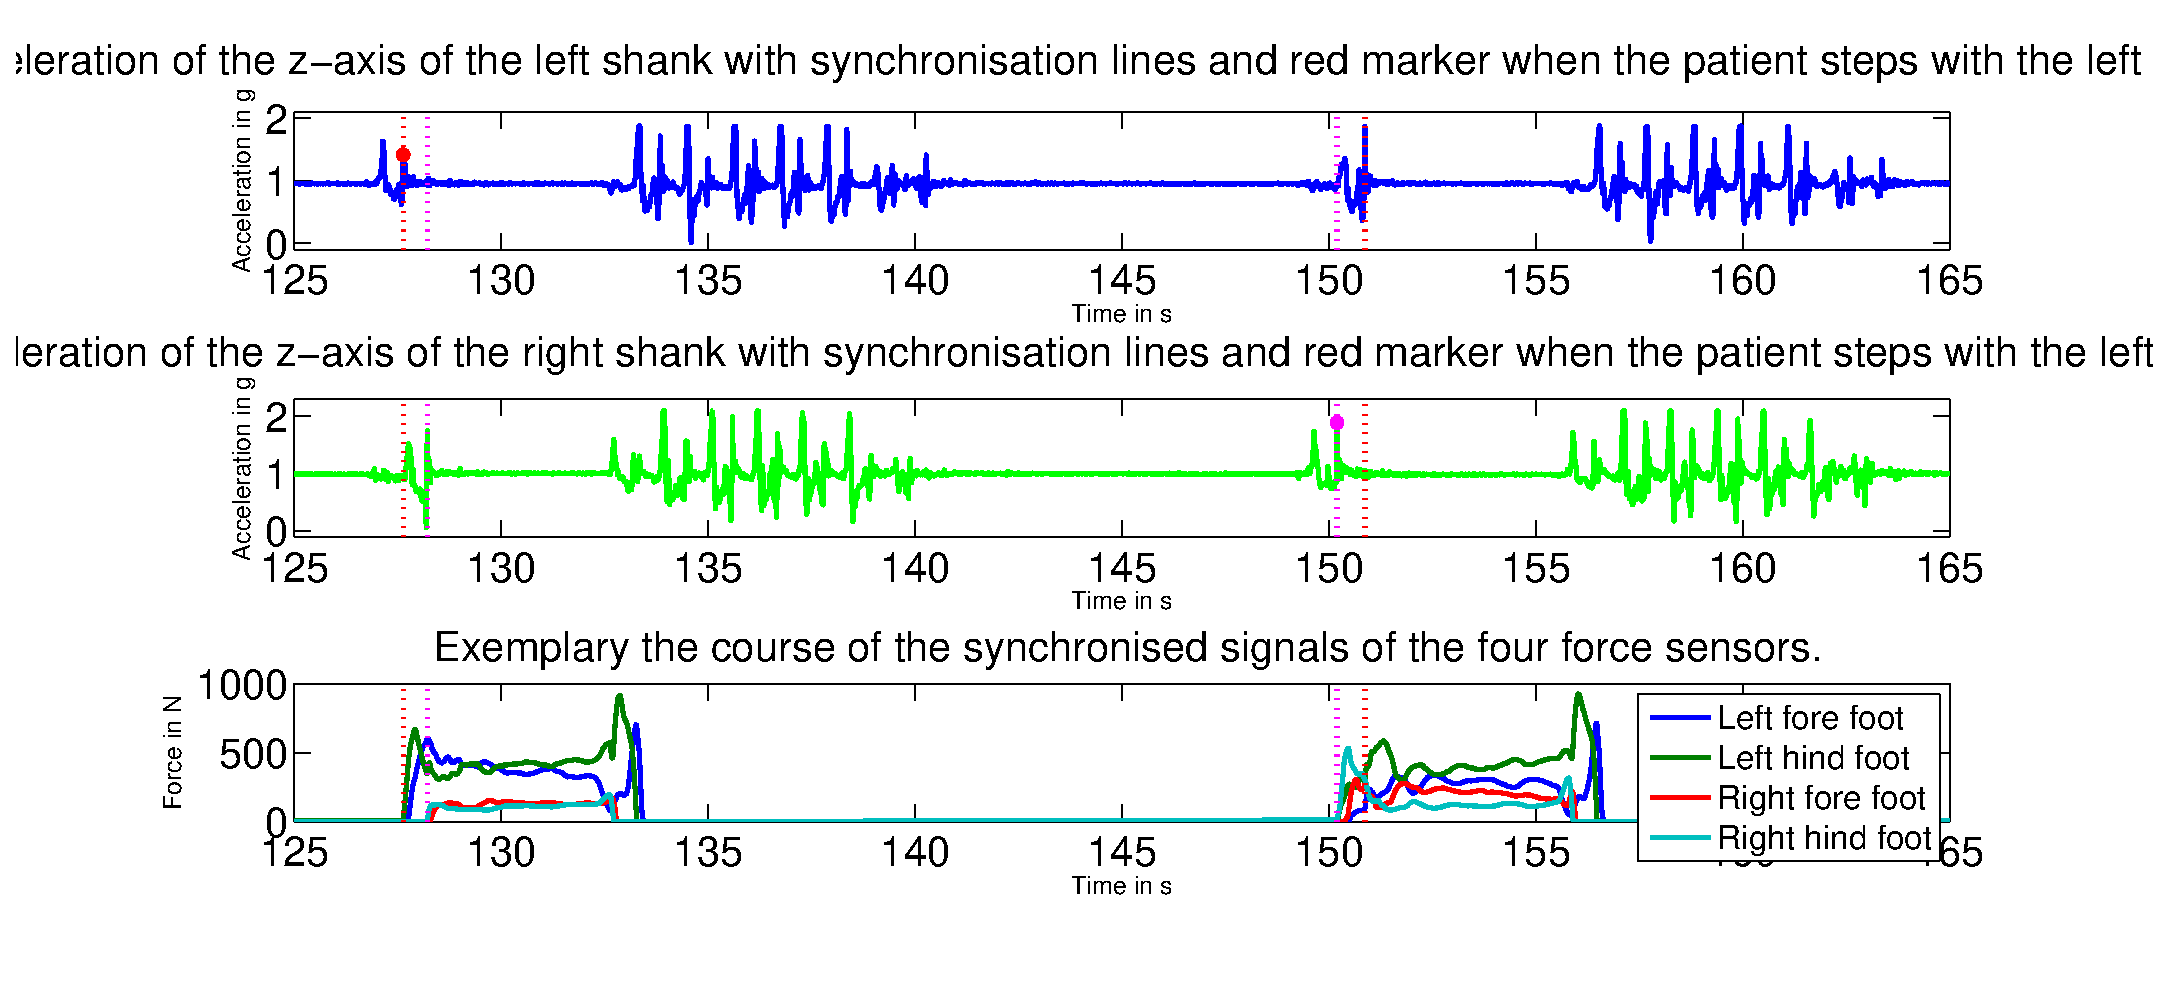
\epsfig{file=figures/Synchronisation/sinchronisedSignals, width=18cm, height=10cm}
	\caption{Synchronisation of the Force from the FP and Acceleration from the GW System .}
	\label{fig:sinchronisedSignals}
\end{figure}


\section{APA analysis}
\subsection{Introduction and chapter's structure}

Anticipatory postural adjustments (APAs)  represents balance control that help to stabilise and mobilise the body based on anticipation of forces accompanying voluntary movement such as volitional lifting of the foot during step initiation \cite{Mancini2010}. Step initiation requires a tight proprioceptive coordination between motor commands for postural adjustments and for stepping, so APAs act to accelerate the center of pressure over the stance foot immediately prior to gait \cite{Mancini2009}.

APAs, before gait initiation, are bradykinetic in advanced Parkinson’s disease and may be one of the factor associated with ‘start hesitation’ \cite{Mancini2009}.

Early identification in patients with PD is important because new neuroprotective medications are being tested to slow the progression of this disease and it is necessary to begin early in the disease, prior to significant loss of neurons \cite{Mancini2012}. 

Currently, the most common way to evaluate postural control in the clinic is to use clinical rating scales that are limited by clinician bias, insensitivity to mild impairments and poor reliability. These limitations are serious problems for clinicians and researchers who want to monitor the disease progression, determine intervention efficacy or treat people with mild balance deficits \cite{Mancini2012} .

Technology avaiable for clinicians and researchers to mesure APAs is generally force plate for the analysis of center of pressure. However, force plate is quite large and expensive and requires a proper installation that may not be practical for clinical use. Thus, Body-worn accelerometers have been proposed as a portable, low-cost alternative to a force plate for measurements of postural sway \cite{Mancini2012} .
 
Therefore, along this chapter we will do a comparative study of the measurements obtained of the force plate as well as accelerometers that make up the Gait Watch system. Also, we will compare these measurements with gyroscopes data that form part of this system too, in order to determine what sensors give us the more accurate results.

\subsection{FP and GW Signals}
As we said in the before chapter, leg's acceleration in the Gait Watch System as well as force in the Platform System are the most accurate signals to detect when the step happens. This is very important to do the synchronisation of the all signals of the system. However, the most interesting signals since a medical point of view are the trunk acceleration and the displacement of the center of pressure.

This is because we can observe the Anticipatory Postural Adjustments in these signals, i.e the body movements before stepping. According to prior studies and priori criteria it is thought that could be a good way to characterise the APAs.
Therefore, the first process to carry out is the analysis of the trunk acceleration and COP to determine if there is some pattern and whether we will be able to use them to obtain information about the patients.

The first step that needs to be carried out is establish the axes in the platform to define the position over it. The X axis points forward, not existing negatives values because the range is between 0 and 510 mm, that is the platform’s dimension in this direction. The Y axis is pointing to the right of the patient, so the positives values indicate a movement toward right with regard to the midline. Comparably, the negatives values are found when the movement is toward the left \ref{fig:axesFP}.
\begin{figure}[H]
	\centering
	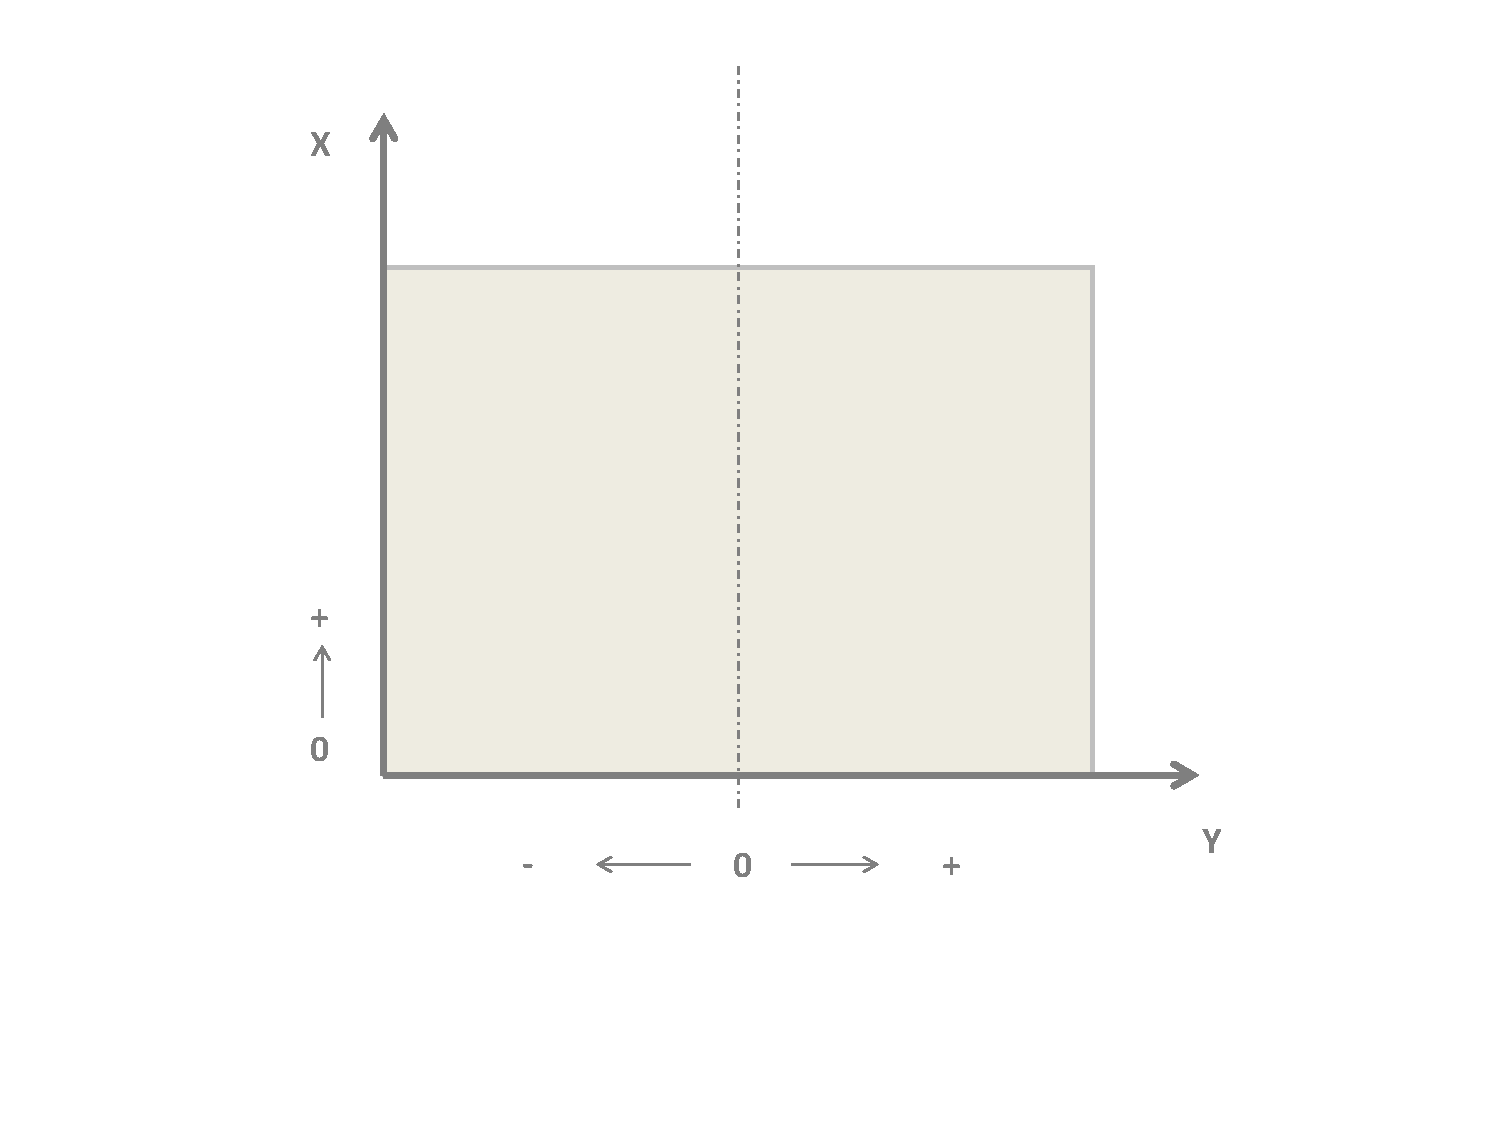
\epsfig{file=figures/APA_analysis/axesFP.pdf,  width=0.6\textwidth}
	\caption{Definition of the axes in the Platform.}
	\label{fig:axesFP}
\end{figure}
Now, for the GaitWatch System we have to determine the orientation of the axes of the body frame that we wish to use, as well as the orientation of the rotation around those axes. The most popular configurations is to set the X axis pointing forwards, the Y axis pointing to the right and the Z axis pointing down. This configuration follows the rule of the right hand for the orientation of the axes and the corkscrew rule for the rotation \cite{OlivaresBotzel2013}. 

Since we will be using the GaitWatch device to monitor gait, then we need its X axis to point to the front of the patient, the Y axis pointing to the right  of the patient, and the Z axis to the floor \ref{fig:axesGW} \cite{OlivaresBotzel2013}.

Once we have identified the axes of the accelerometers, we now proceed to identify the axes of the gyroscopes and their orientation. By convention, as it is depicted in \ref{fig:axesGW}, the sense of the rotation around a given axis is positive when the axis is pointing forwards (from the perspective of the user) and it is turned to the right. So, in this case the rotation is positive toward right\ref{fig:axesGW}. Analogously, the rotation is negative when it is turned to the left.

\begin{figure}[H]
	\centering
	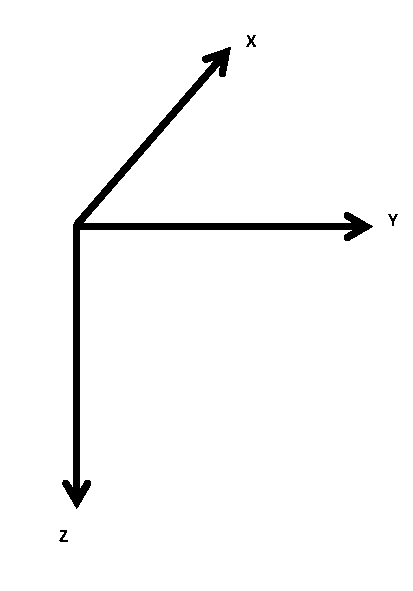
\epsfig{file=figures/APA_analysis/axesGW.pdf, width=0.2\textwidth}
	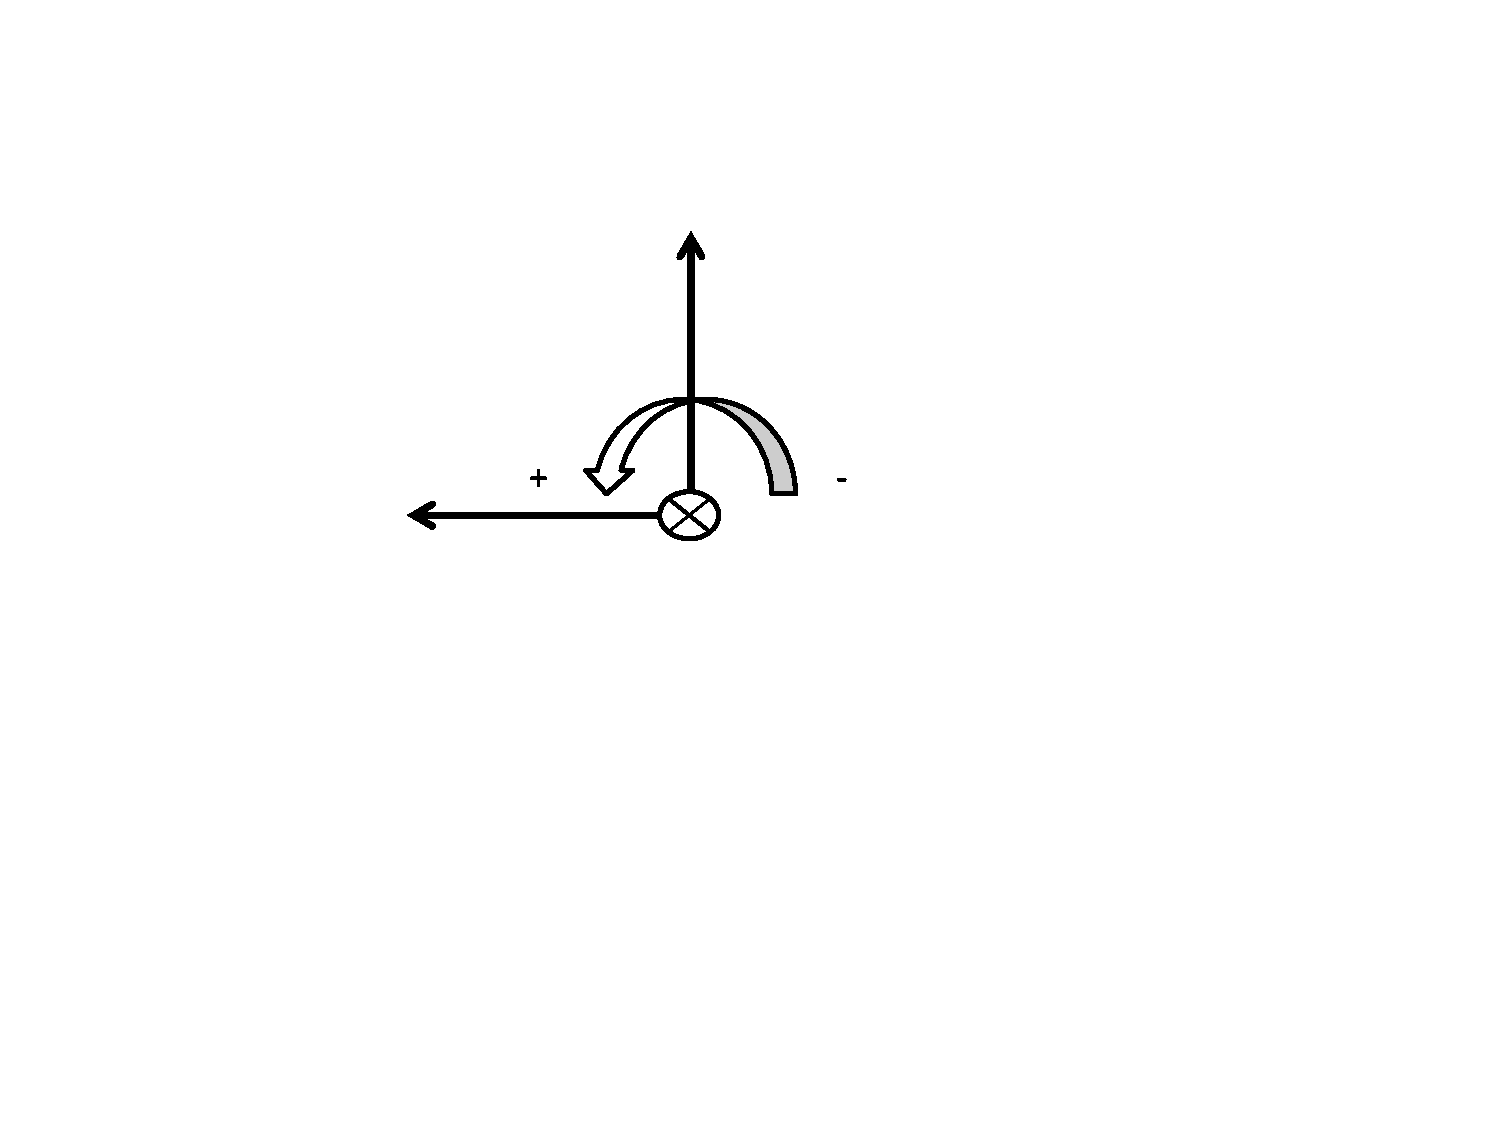
\epsfig{file=figures/APA_analysis/axesGWGyro.pdf, width=0.25\textwidth}
	\caption{Definition of the axes in the accelerometers ans gyroscopes (left). Orientation of the axis rotation in gyroscopes (right).}
	\label{fig:axesGW}
\end{figure}

We have to differentiate between the front-back movement and the right-left movement. In the first of the case, we have the acceleration in X axis and the Antero-Posterior COP. In the another case, the movement is traced by the acceleration in Y axis and the Medio-Lateral  COP.




Whether we focus in the Antero-Posterior movement, the body is displaced forward while the step is being completed. Thus, the center of mass is shifted backward in this period of the movement. In the case of center of pressure, we can find first  movement backward to gain momentum and after that  COP moves forwards under the stance of the foot \ref{fig:AP_AccX}.



\begin{figure}[H]
	\centering
	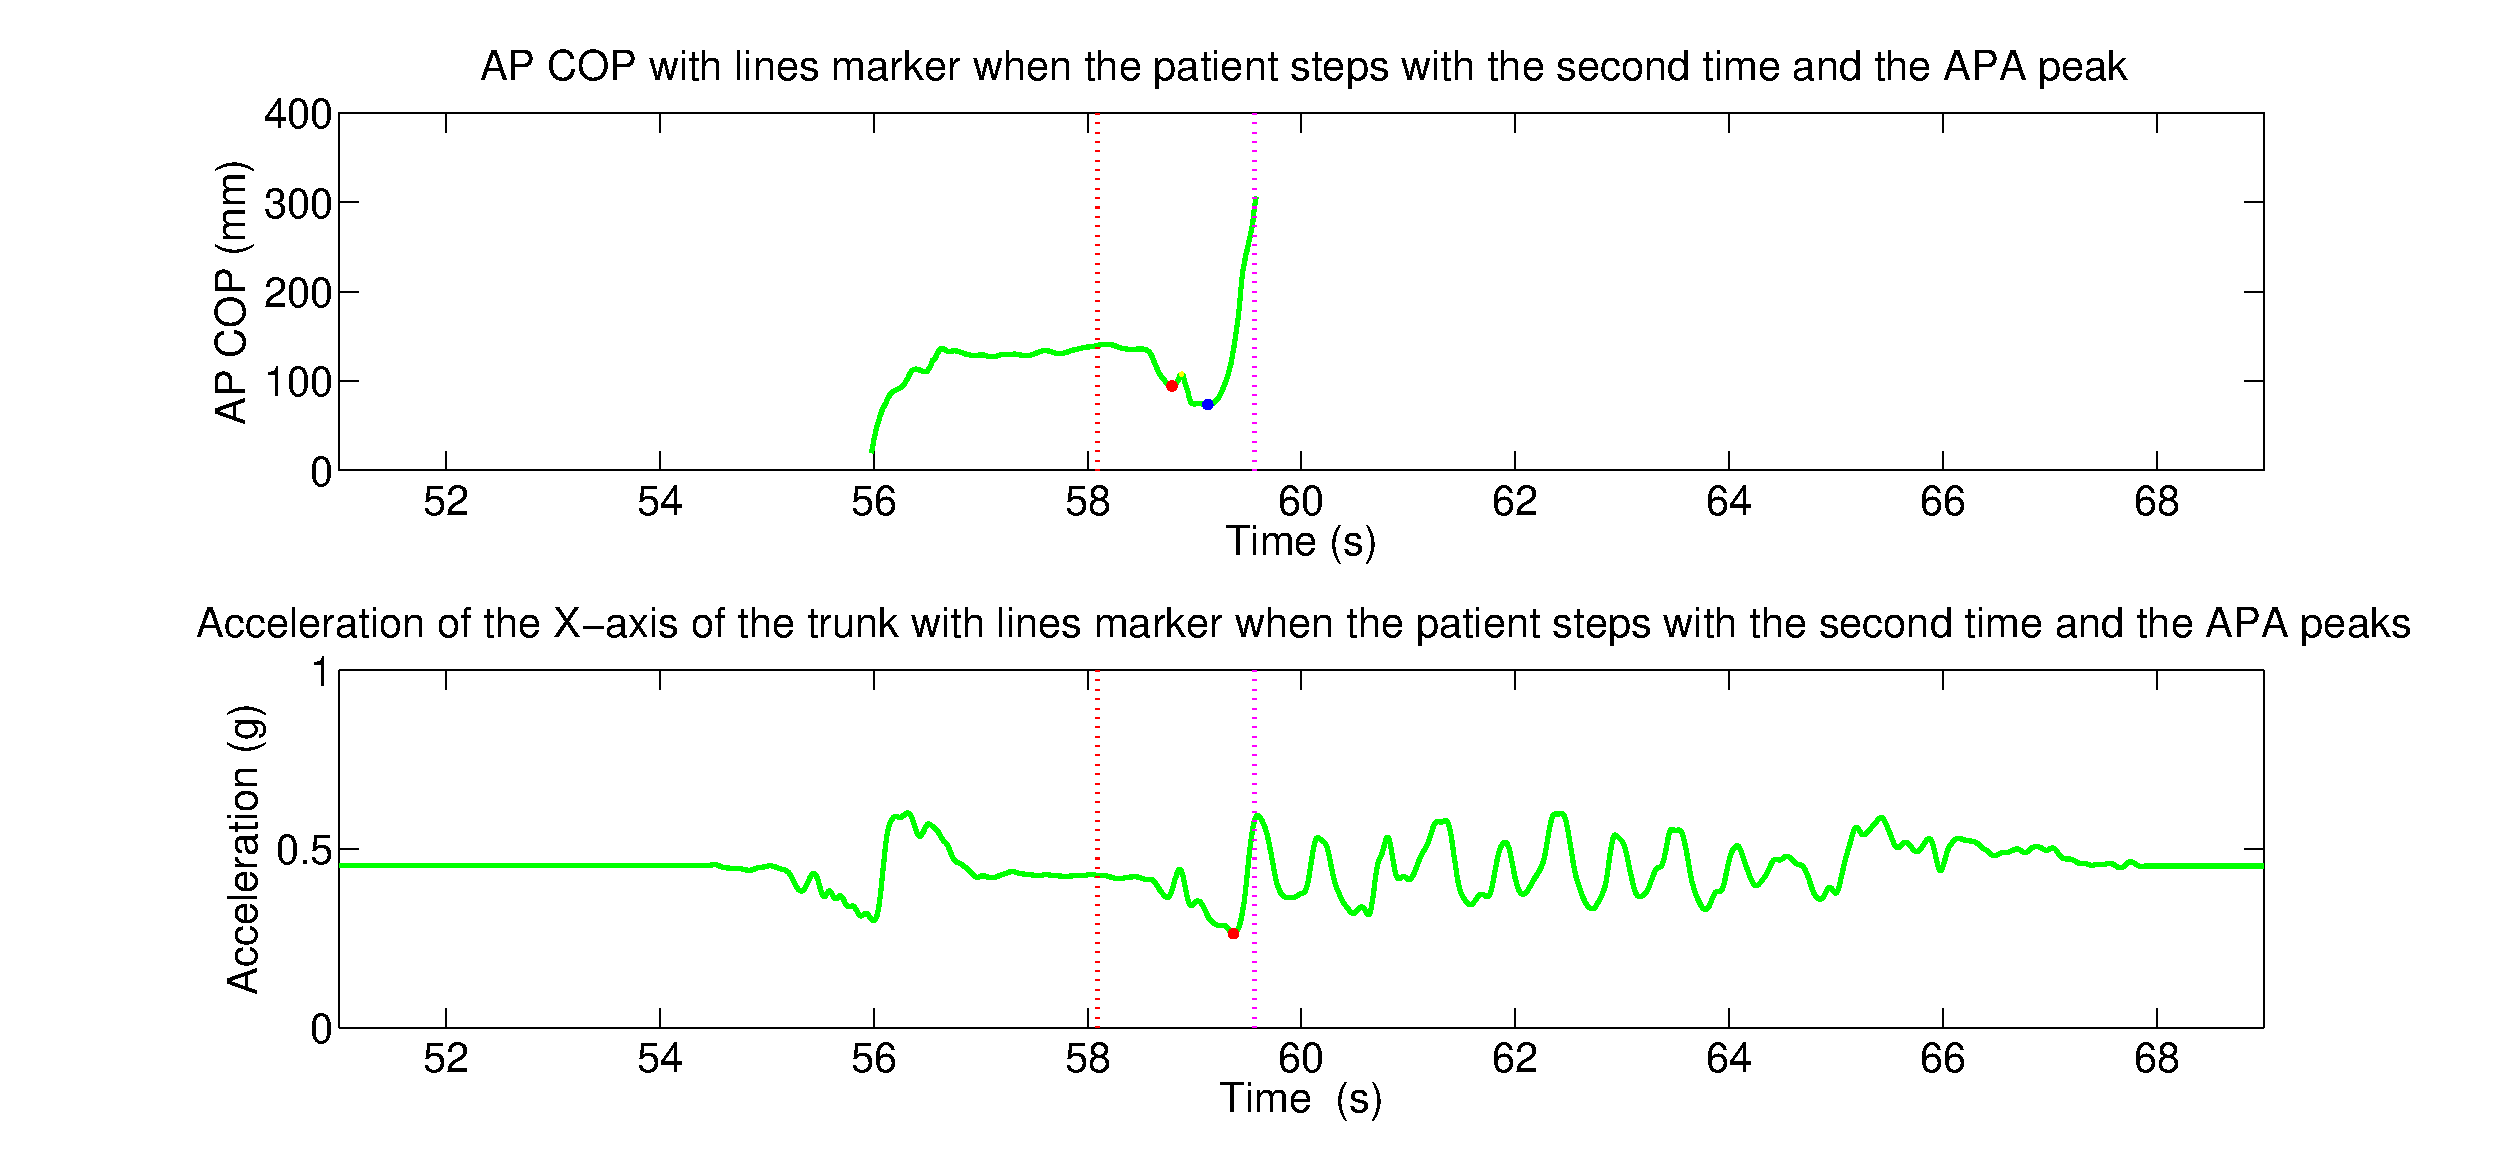
\epsfig{file=figures/APA_analysis/AP_AccX, width=1\textwidth}
	\caption{COP and acceleration in Antero-Posterior direction.}
	\label{fig:AP_AccX}
\end{figure}

From a kinematic point of view, the trunk is moved anteriorly while the patient steps. Therefore, there will be a peak of acceleration in the X axis pointing forward, so we will find a ‘negative’ peak at this moment because the acceleration vector points in the opposite direction to the movement. After that, there is a positive peak that corresponds with the direction change just when the step finishes. 

Also, we can observe a pattern due to all movements before stepping follows a only trace approximately. The pattern of the acceleration in the X-axis (anterior-posterior movement) is always the same, regardless of the leg which the patient starts to walk.

Moreover, we discern differences in the Medio-Lateral direction regarding the foot with which the step is done. 

If the patient starts to step with the right foot, the center of mass is accelerated toward left because the major body heigh is located in the foot over the ground. However, the center of pressure is shifted toward right and then the COP displaces mediolaterally to left, toward the foot is contact with the ground. For the acceleration in the Y axis, there is a negative peak because the movement is towards right and the acceleration vector points in the opposite direction, with negatives values. After this, we find a negative peak due to the change of direction\ref{fig:ML_AccY_right}. 

\begin{figure}[H]
	\centering
	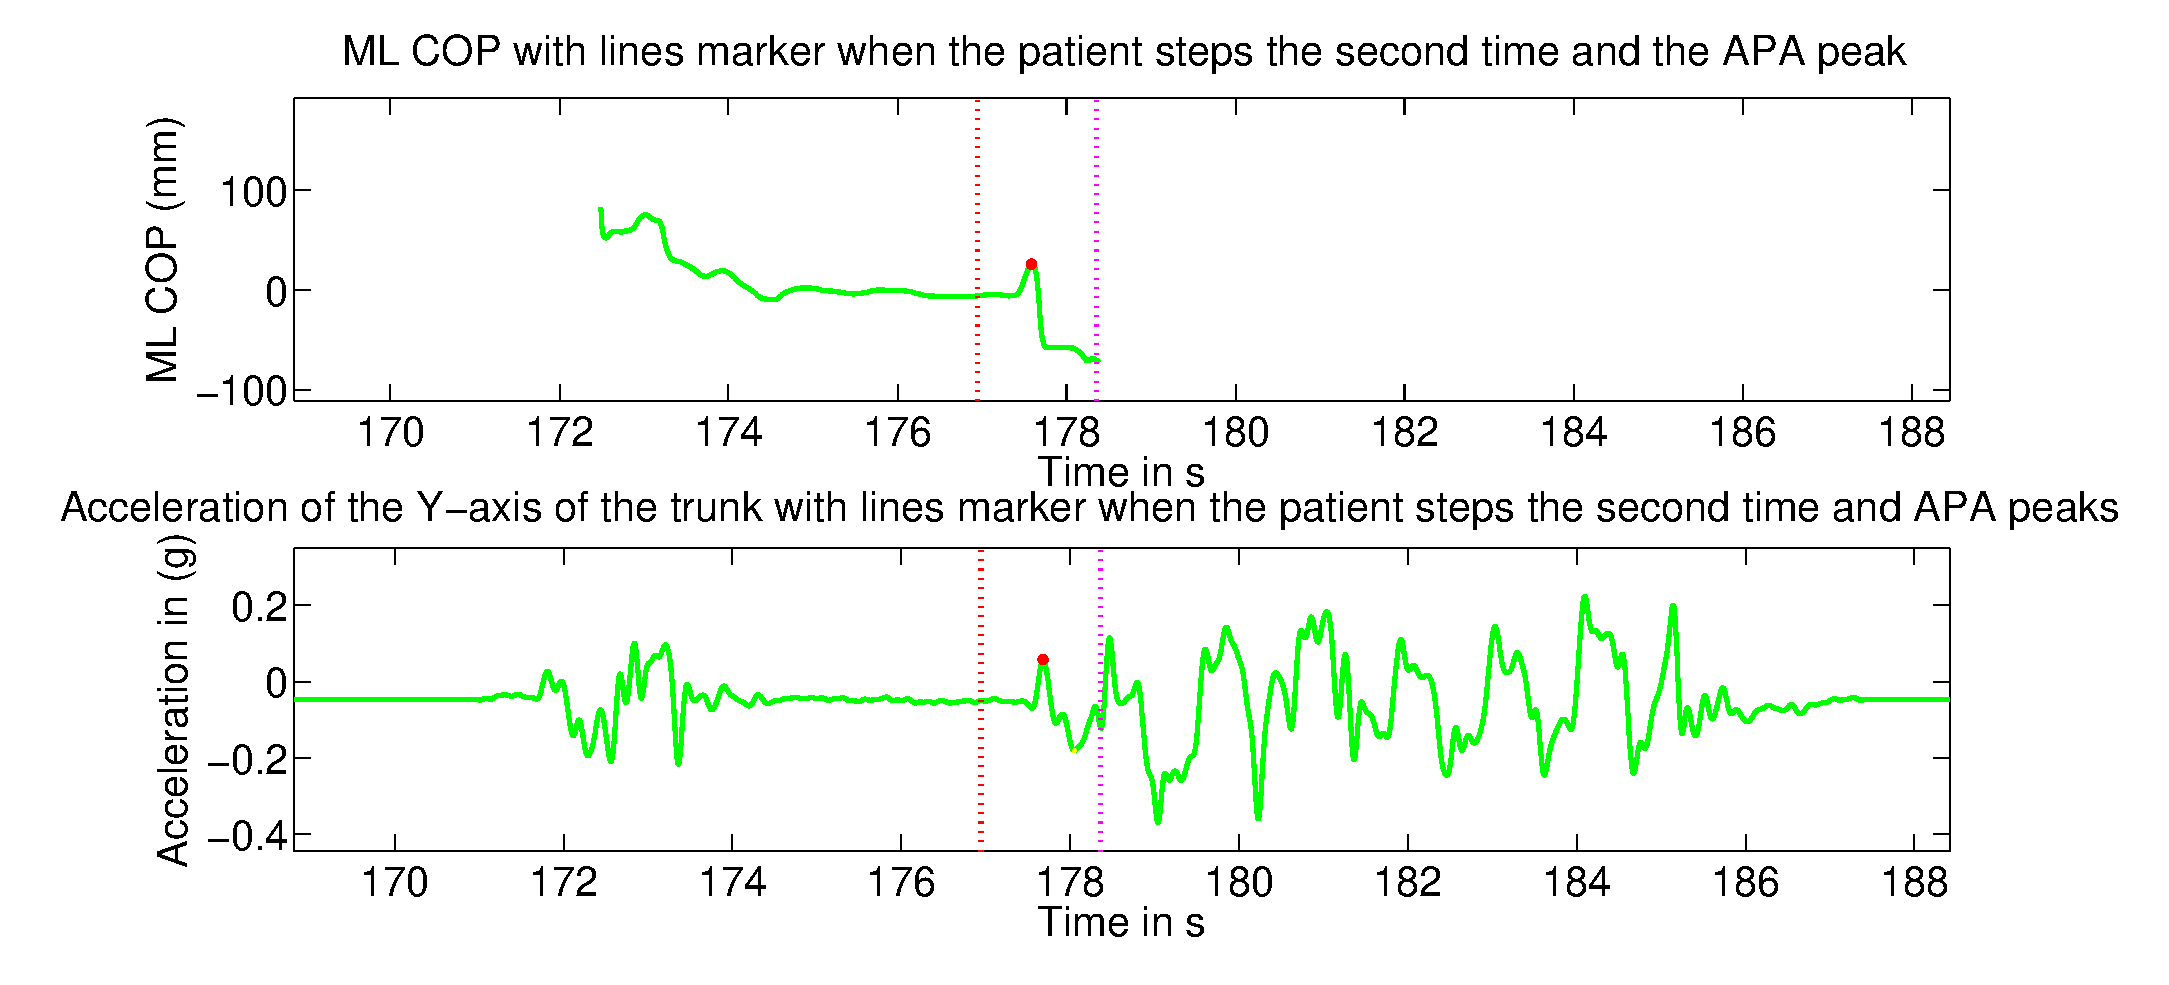
\epsfig{file=figures/APA_analysis/ML_AccY_right, width=1\textwidth}
	\caption{COP and acceleration in Medio-Lateral direction when patient steps with the right foot.}
	\label{fig:ML_AccY_right}
\end{figure}

If the patient starts to step with the left foot, the movements are the same than in the prior case unless the movement directions are just the opposite. We can perceive this in \ref{fig:ML_AccY_left}

\begin{figure}[H]
	\centering
	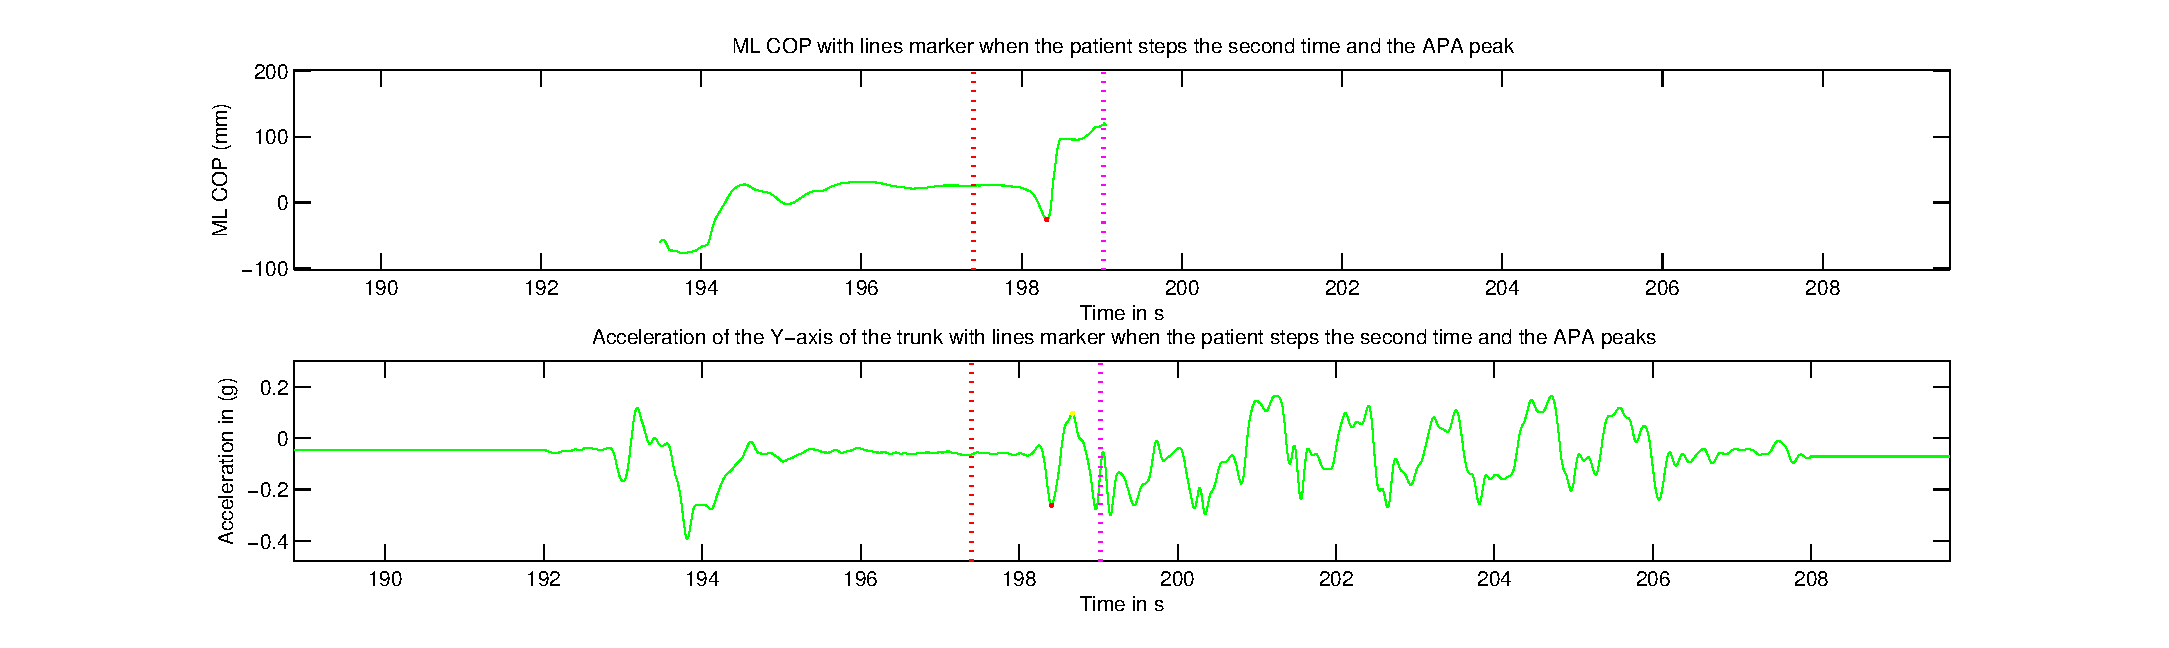
\epsfig{file=figures/APA_analysis/ML_AccY_left, width=1\textwidth}
	\caption{COP and acceleration in Medio-Lateral direction when patient steps with the left foot.}
	\label{fig:ML_AccY_left}
\end{figure}

To sum up, we have to differentiate between the foot which the step is done (stepping foot) and the foot over the ground (stance foot) to understand the behaviour of the APAs. The center of mass (COM) is shifted toward the stance foot to maintain the equilibrium during the balance phase. The center of pressure (COP) is divided in differents phases. Firstly, the COP moves toward the stepping foot and backward to generate the momentum to step (S1 period). Hereafter, the COP is displaced toward the stance foot. This happens at time when the other foot is in the air (S2 period). Finally, the COP moves forward and under the stance foot (S3 period) \ref{fig:trajectoryCOP}.

Bearing in mind the same phases for the acceleration than in the above case, in the first period (S1 period) the body is accelerated forward while the momentum is generated to step. After, the trunk is slightly accelerated toward left (S2 period) and finally, in the last period the body is moved fordward anf toward rigth to complete the step (S3 period) \ref{fig:trajectoryAcc}.  

\begin{figure}[H]
	\centering
	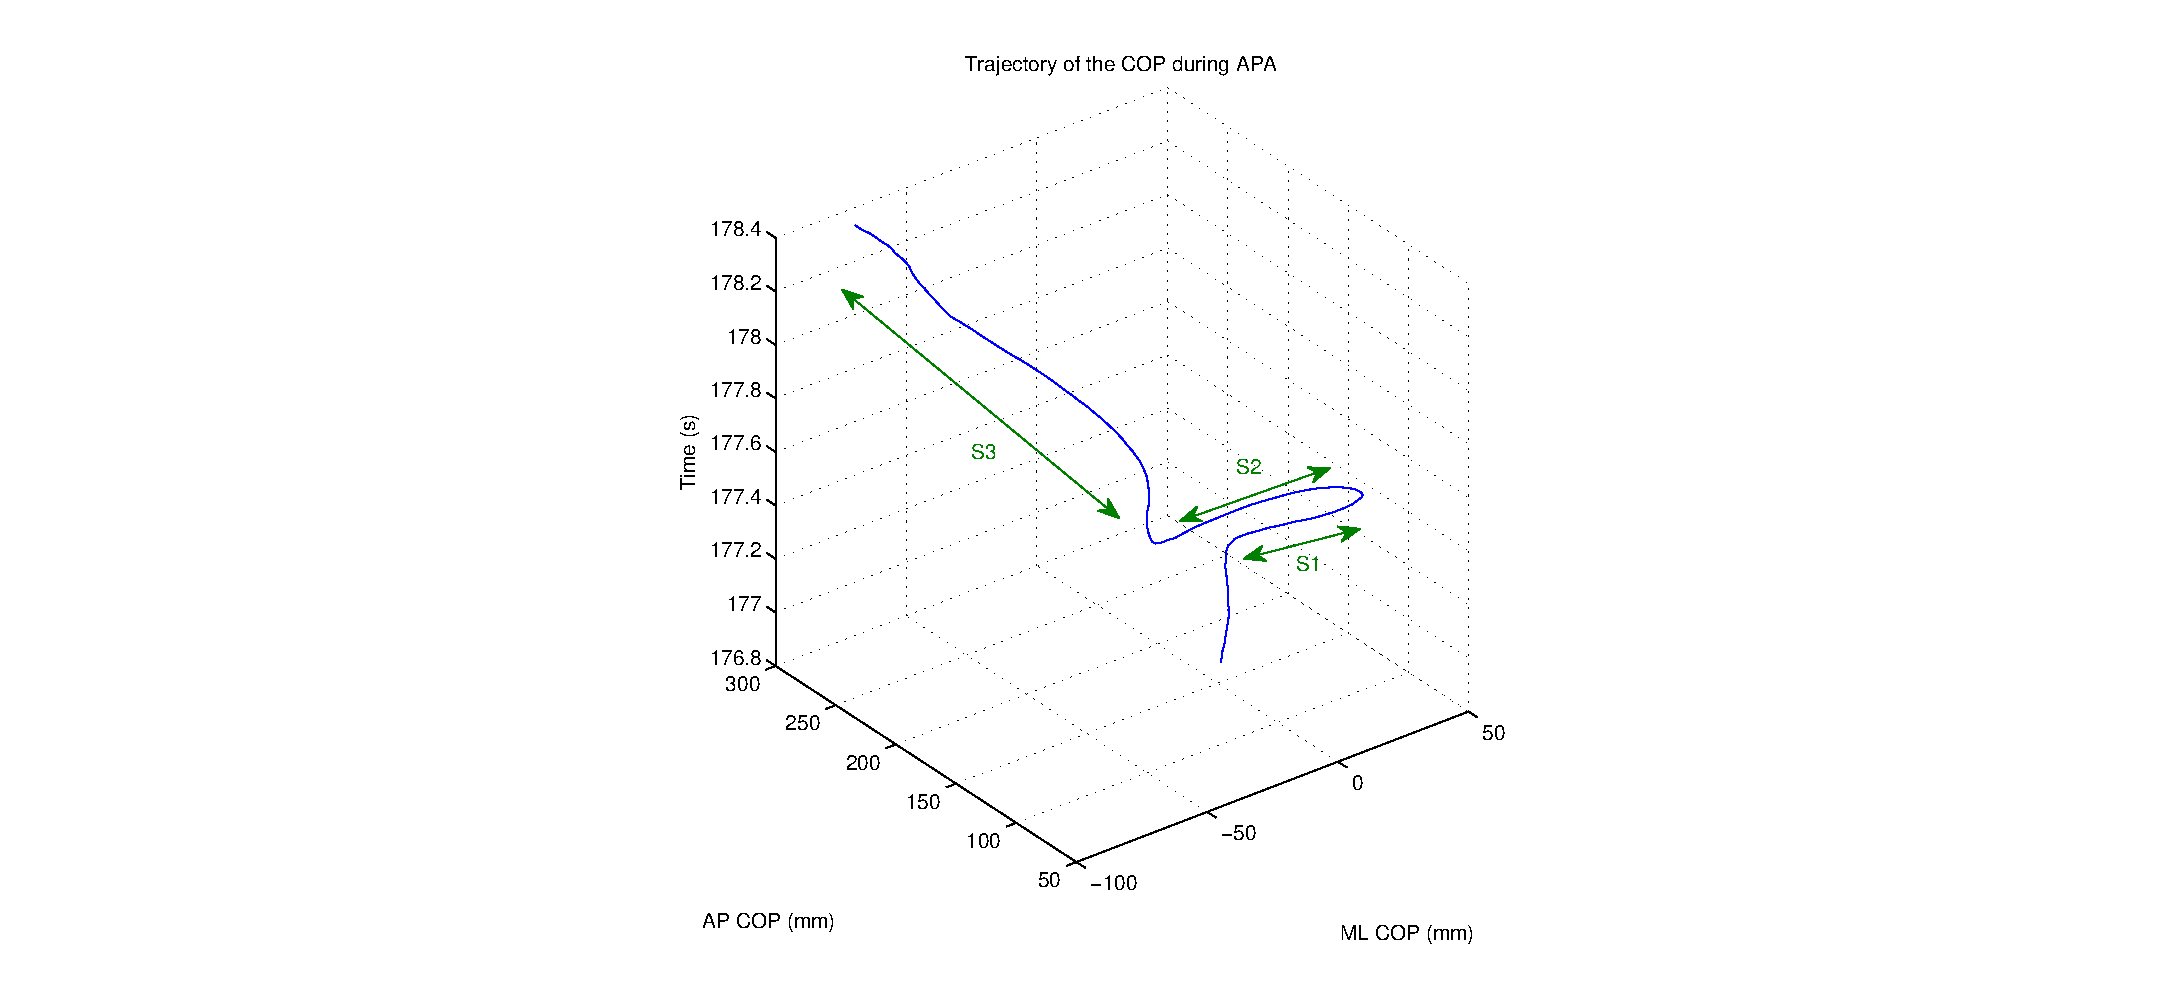
\epsfig{file=figures/APA_analysis/trajectoryCOP, width=0.5\textwidth}
	\caption{Trajectory of COP when patient steps with the right foot.}
	\label{fig:trajectoryCOP}
\end{figure} 
                 
\begin{figure}[H]
	\centering
	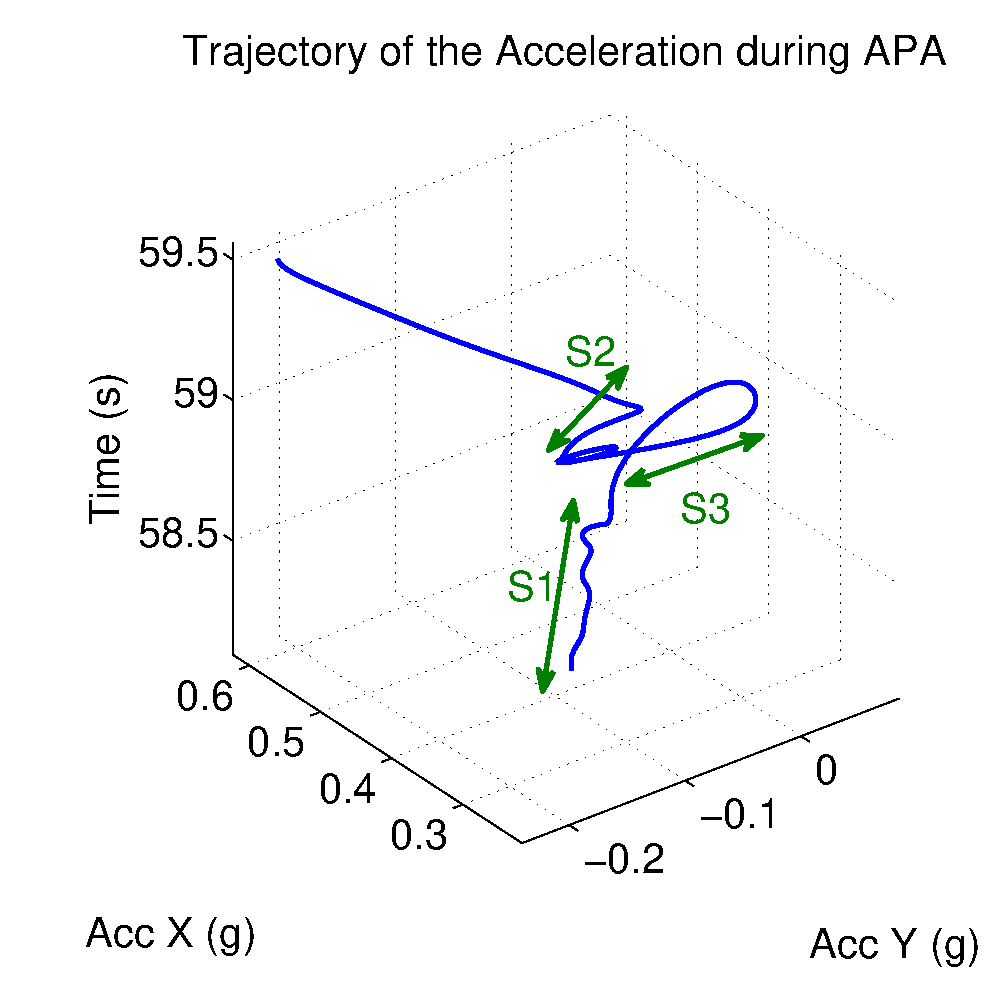
\epsfig{file=figures/APA_analysis/trajectoryAcc, width=0.6\textwidth}
	\caption{Trajectory of acceleration when patient steps with the right foot.}
	\label{fig:trajectoryAcc}
\end{figure} 

The behaviour of the gyroscope signals is very similar to the accelerometer signals but this case we are measuring a turn forward or backward and toward right or left. 

\begin{figure}[H]
	\centering
	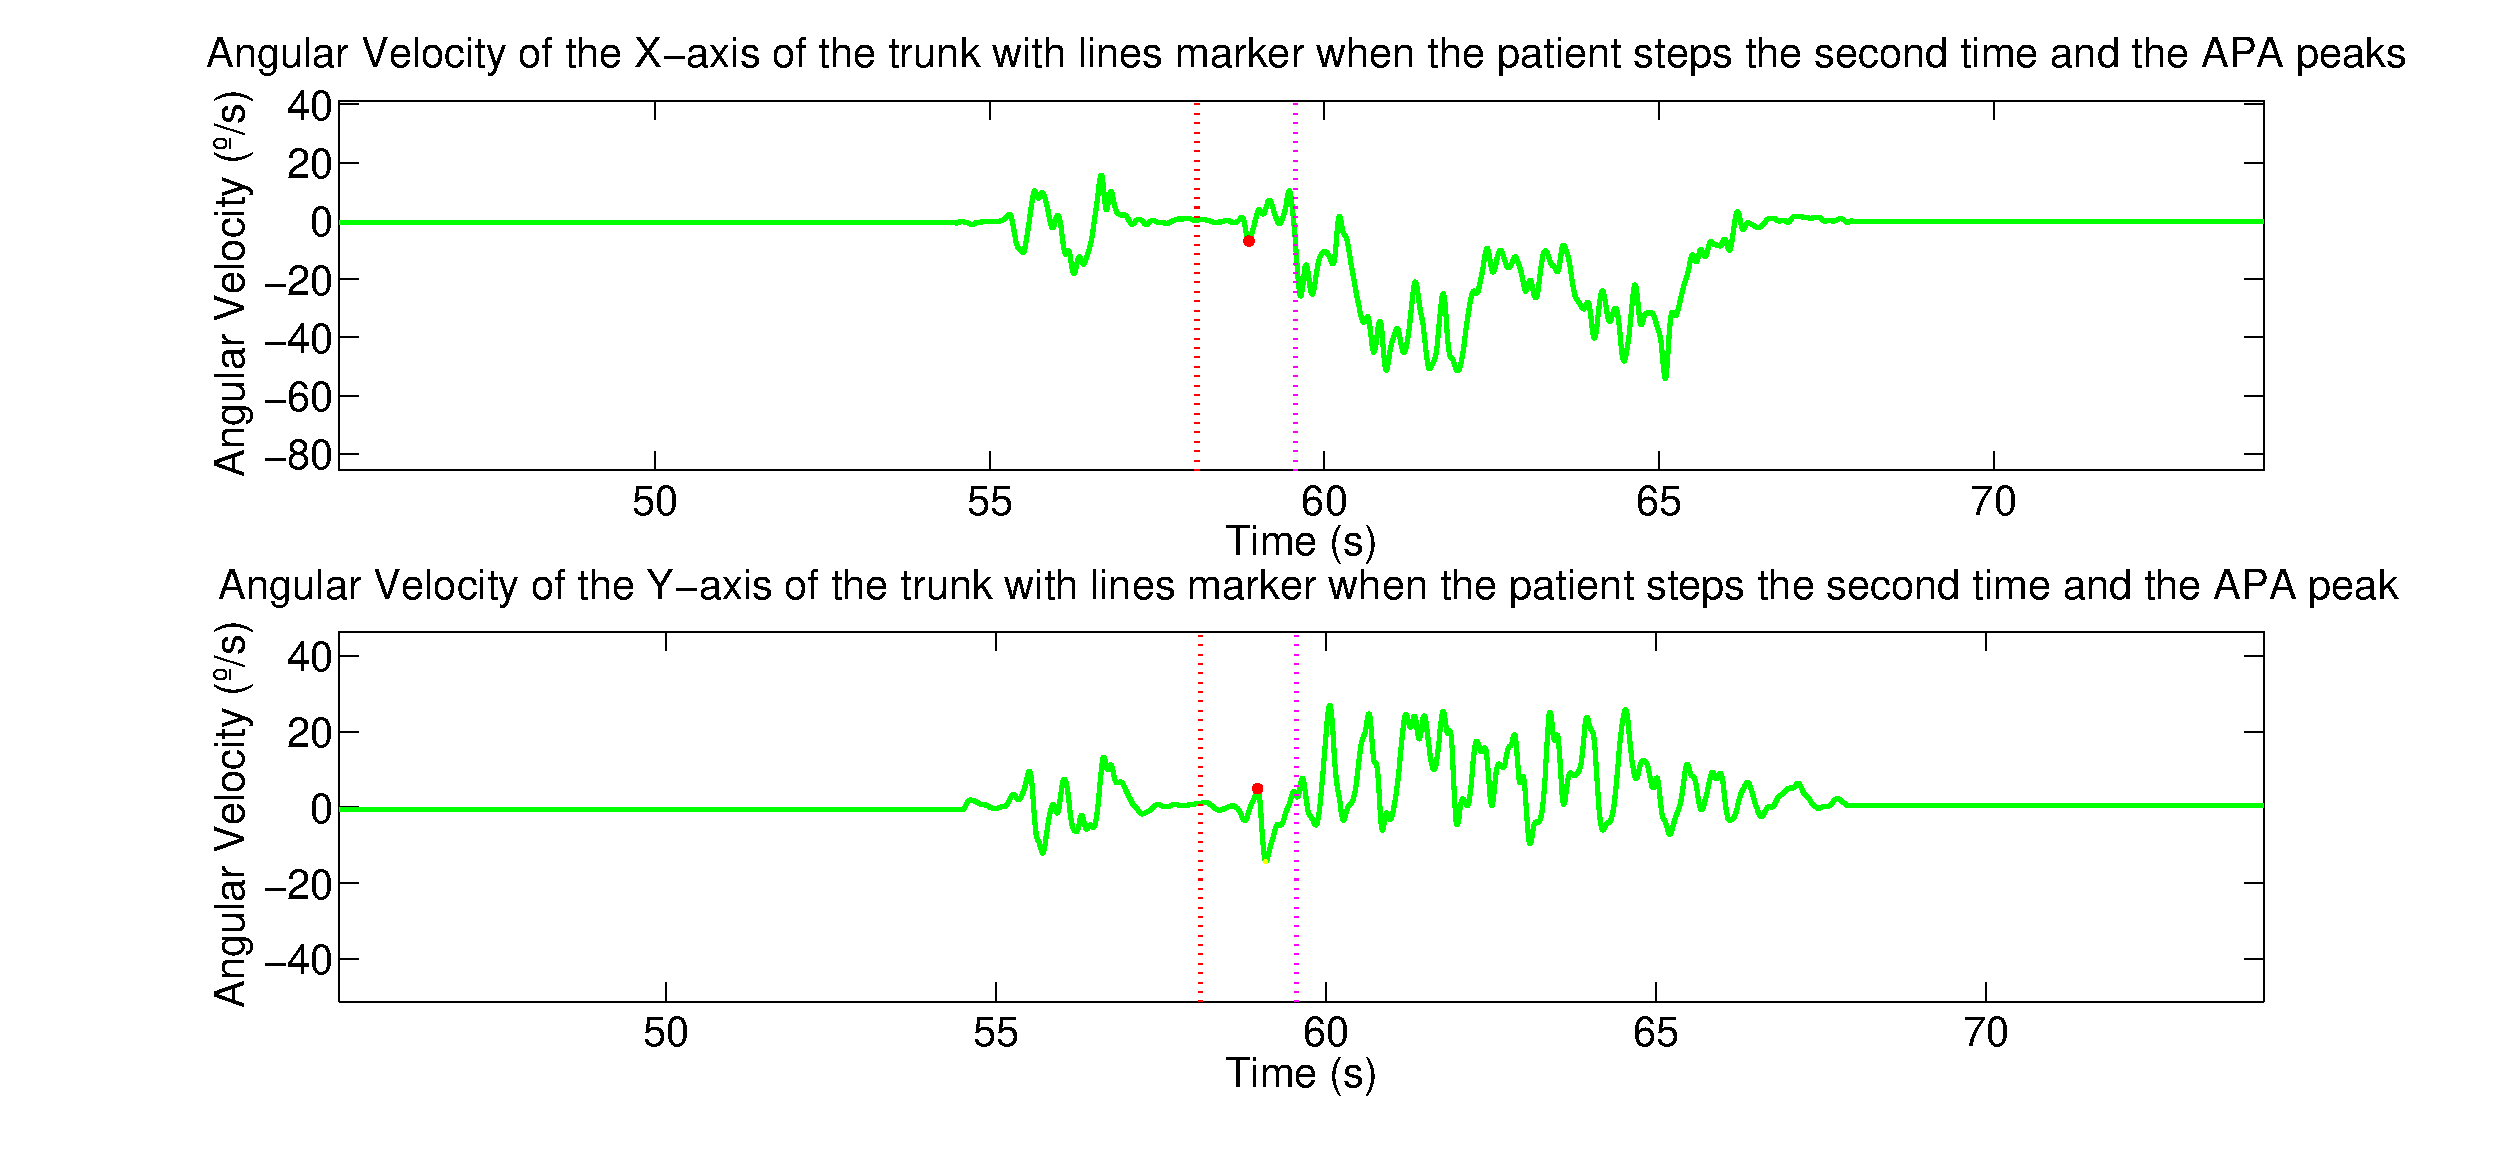
\epsfig{file=figures/APA_analysis/GyroTrunk, width=1\textwidth}
	\caption{Angular Velocity when patient steps with the right foot.}
	\label{fig:GyroTrunk}
\end{figure} 

There are a negative peak when patient turns to backward before walking in the Antero-Posterior direction. Besides, it will be a negative peak when patient is shifted toward right and positive in the case that the turn was done to left in the Y axis.


\subsection{PCA}
One of the most difficulties inherent in multivariate stadistics is the task of the features extraction to obtain the most relevant information from the original data and represent that information in a lower dimensionality space.

PCA is a qualitative rigorous method for achieving this and it has been widely applied in gait analysis both for the reduction of redundant information and the interpretation of multiple gait signals \cite{PCA}.

This method attempts to represent the data efficiently by descomposing a data space into a linear combination of a small collectionof bases collection of bases consisting of orthogonal axes that maximally decorrelate the data \cite{Jeon}.

Given  set of centered N-dimensional training gait samples 
$ x_{j}, j=1,...,M     x \in$ such that $ R_{N} $ and $ R=\sum_{k=1}^{M}x_{j}=0 $
	
Where M represents the number of gait samples and N is the number of input values. The $ x_{j} $ vectors are aligned in the data matrix X. Also, the data have to be center so it's necessary to extract the average of the each set.
\begin{figure}[H]
	\centering
	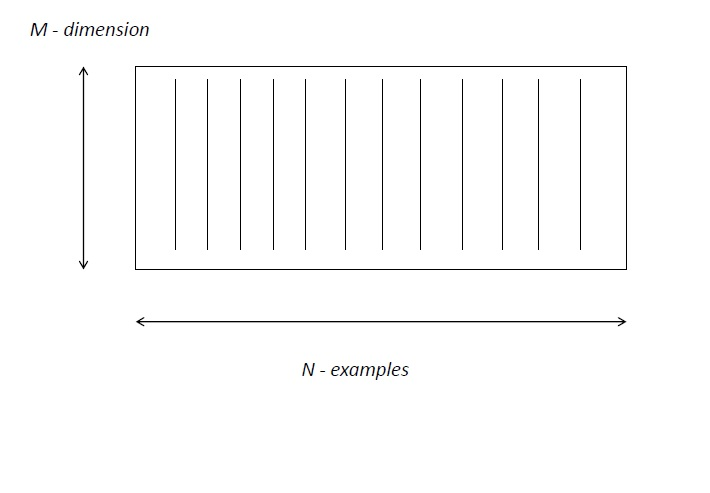
\epsfig{file=imagenes/PCA.jpg, width=10cm}
	\caption{Data matrix X with M rows and N colums.}
	\label{fig:matrixPCA}
\end{figure}

The projection of the \textit{j-th} vector $ x_{j} $ onto the vector \textit{'u'} can be calculated in the folowing way:

\begin{equation}
	\label{projections}
	p_{j}=\overrightarrow{u}^{T}\overrightarrow{x}_{j}=\sum_{i=1}^{N}u_{i}x_{ij}	
\end{equation}

We want to find a direction \textit{'u'} that maximizes the variance of the projections of all input vectors. That funtion to maximize is:

\begin{equation}
	\label{maxfunction}
	J^{PCA}(\overrightarrow{u})=\sigma^{2}(p_{j})=\dfrac{1}{M}\sum_{j=1}^{N}(p_{j}-\bar{p})^{2}=...=\overrightarrow{u}^{T}C\overrightarrow{u}	
\end{equation}

Where C is the covariance matrix of the data matrix X.

$$C=\dfrac{1}{N}\hat{X}\hat{X}^{T}$$

Using the technique of Lagrange multipliers, the solution to the maximization problem is to compute the eigenvectors and eigenvalues of the covariance matrix.

Thus, we have to solve the following eigvector problem:
\begin{equation}
	\label{eigenproblem}
	\Lambda U=C^{'} U
\end{equation}

In such a way the orthonormal matrix U contains the eigenvectors $u_{1}, u_{2},...u_{N}$ in its colums and the diagonal matrix $\Lambda$ contains the eigenvalues $\lambda_{1}, \lambda_{2},...,\lambda_{N}$ on its diagonal.

The eigenvalues and the eigenvectors are arranged with respect to the descending order of the eigen values, thus $\lambda_{1}\eqslantgtr\lambda_{2}\eqslantgtr...\eqslantgtr\lambda_{N}$

Therefore, the most variability of the input random vector is contained in the first eigenvectors. Hence, the eigenvectors are called principal vectors.

So U can be used as a linear transformation to project the original data of high dimension into a space of lower dimension.

$$P=U^T\bar{X}$$

In terms of gait feature extration by choosing the first two eigenvectors, PCA can directly perform the dimensional reduction\cite{Jeon}.
We can use this new information to do a classification. Tha classification can be achieved through a SVM which separates a given set of labelled training data with a hyperplane that is maximally distant from the two classes \cite{Gorriz}.

\subsection{Feature extraction}
Automated recognition of gait pattern change is important in medical diagnostic. Thus, in this section we are going to extract and evaluate different gait features as well as methods to obtain them. Feature extraction is a important	to do a good classification of patterns.
The main goal in this chapter is to obtain the relevant information from the platform and inertial sensors synchronised previously and carry out a study comparative between them.

One the one hand we try to figure out whether there is a correlation between the features of both systems and determine if we can use the inertial sensors to characterise the movement without another measure auxiliar  platform.
One the other hand we want to extract useful features that we can use to do a classification between patients and therefore it can be used for diagnosis.

To do this, we will use the data obtained after the synchronisation between Force Plate and Gait Watch signals. Using this signals lets us extract the information easily and compare them.

The next step is to determine when the second step happens. We used as a reference the point when the patient touched the platform to do the synchronisation. However, in this case we have to identify when patient carried out the second step to go down from the platform. We need this part of the signals because it is when we can see the displacements of the center of pressure. To obtain these limits of the signals we use the LTSD algorism. This is applied over the acceleration signal so we can determine the beginning of this period for each cycle. The end of the interval is the point when the patient go down and touch the ground ,i.e when there is not pressure signal over the platform.
Thereupon, we apply a low pass filter to the  Gait Watch signals, i.e signals of the accelerometers and gyroscopes in the trunk. This allows us to delete the low frequencies  of these signals due to the noise of the sensors and get the features properly. Specifically it has been used a low pass filter with a cutoff frequency of 2 Hz.

\begin{figure}[H]
	\centering
	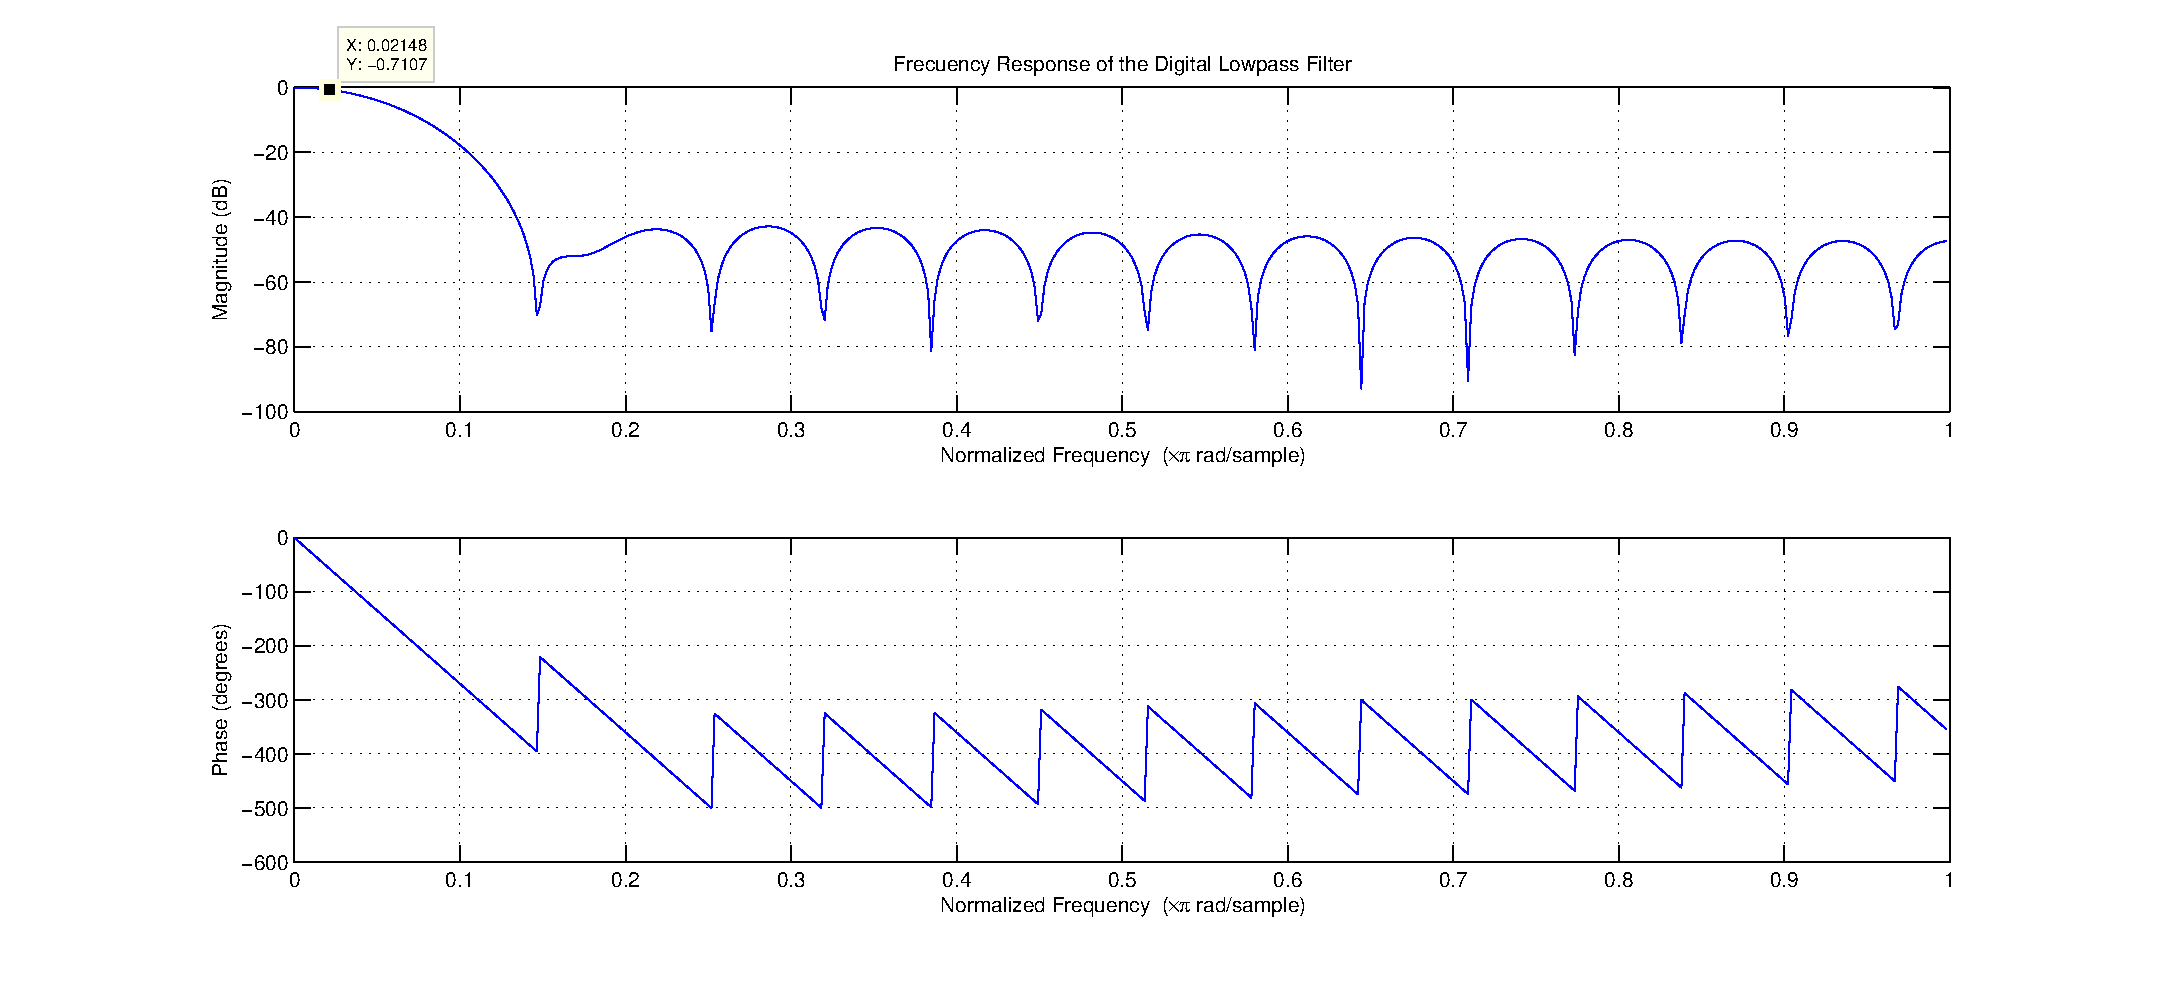
\epsfig{file=figures/Feature_extraction/lowpassFilter, width=18cm, height=10cm}
	\caption{Lowpass Filter with a cutoff frequency of 2Hz}
	\label{fig:lowpassFilter}
\end{figure} 

One the signals have been filtered, we will do the average of all repeat. Typically, the experiment is repeated several times to do a ratio and obtain a single signal for each patient. As we said before, the protocol is repeated about ten times so we have to synchronise this cycles and realise the mean of all them.  First of all, we need determine when the patient steps with the right of left foot. This is important for the signals in the medio-lateral direction because the sing of the signals is the opposite. Thus, if patient does the step with the left foot, the signal will be invert before doing the mean. This fact is detected seeing the last values of the center of pressure because this gives us information about the locatitation of the feet.
When the patient starts to step with left foot, last value of the cycle of ML- COP is positive because the step finishes the pressure is located in the right foot. However, if the patient starts with right foot, the last value of the ML-COP cycle will be negative.

To align the signals, we use cross-correlation between them. The cross-correlation is a mesure of similarity fo two signals as a function of the lag of one relative to the other \cite{Cross-corr}. For discrete function as our case, the cross correlation is defined as:
\begin{equation}
\label{cross-corr}
(f*g)[n]=\varSigma_{m=-\infty}^{\infty} f^{*}[m]g[m+n]
\end{equation}
Where $ f^{*}$ denote the complex conjugate of \textit{f} and \textit{n} is the lag.

Using this method, we can determine the point where the signals are more similar. After this, we can interpolate them and carry out the average between them.

At this point, we have six signals per patient: the center of pressure in the antero-posterior and medio-lateral direction, the acceleration in X and Y axis and the angular velocity in the same axes. Therefore, the next step is extract the features of them. 

We was analysing the Gait Watch and Forceplate signals in the above chapter and determining the most interesting episodes in these signals. So, the first features that we will obtain are the peaks in COP, acceleration and angular velocity. we can see this in the following figures:

\begin{figure}[H]
	\centering
	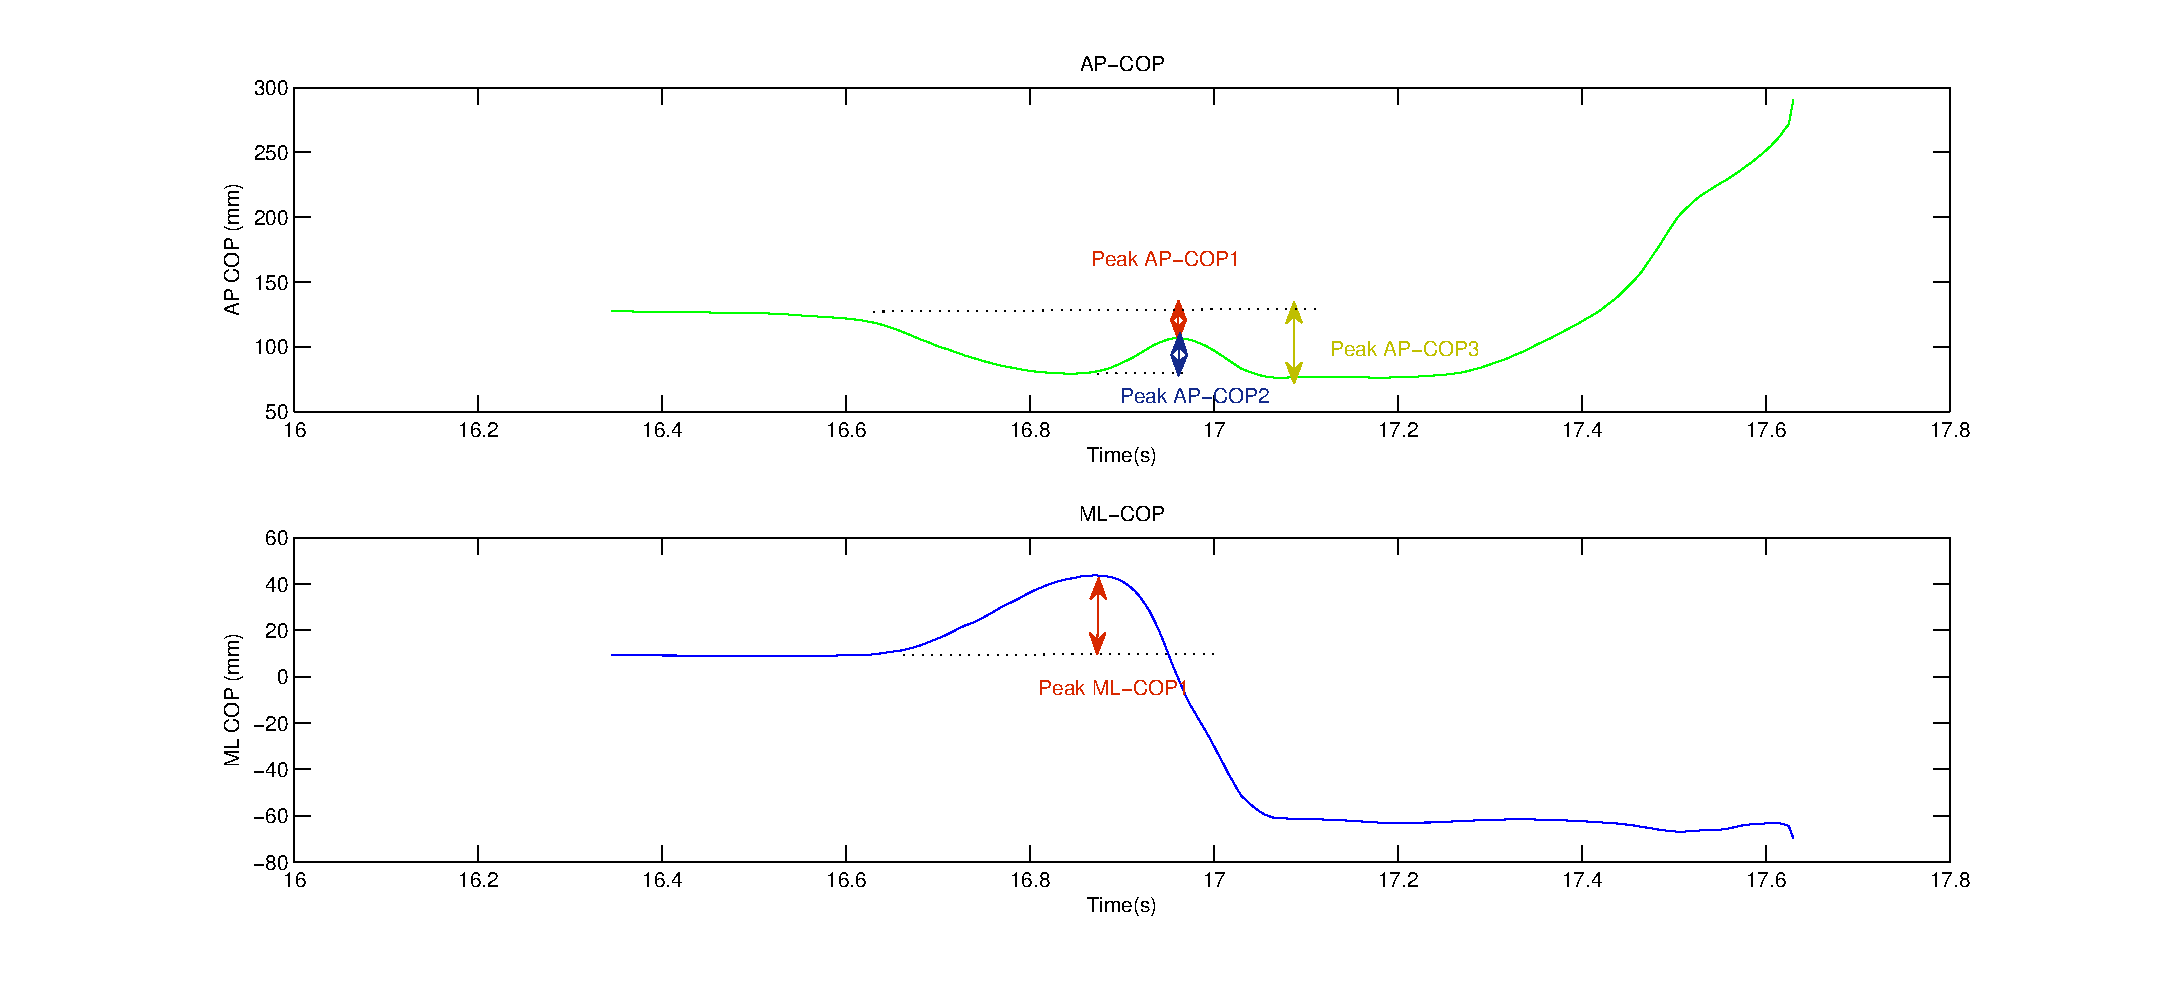
\epsfig{file=figures/Feature_extraction/COP_features, width=18cm}
	\caption{Peaks in the Center of Pressure signals .}
	\label{fig:COP_features}
\end{figure}

\begin{figure}[H]
	\centering
	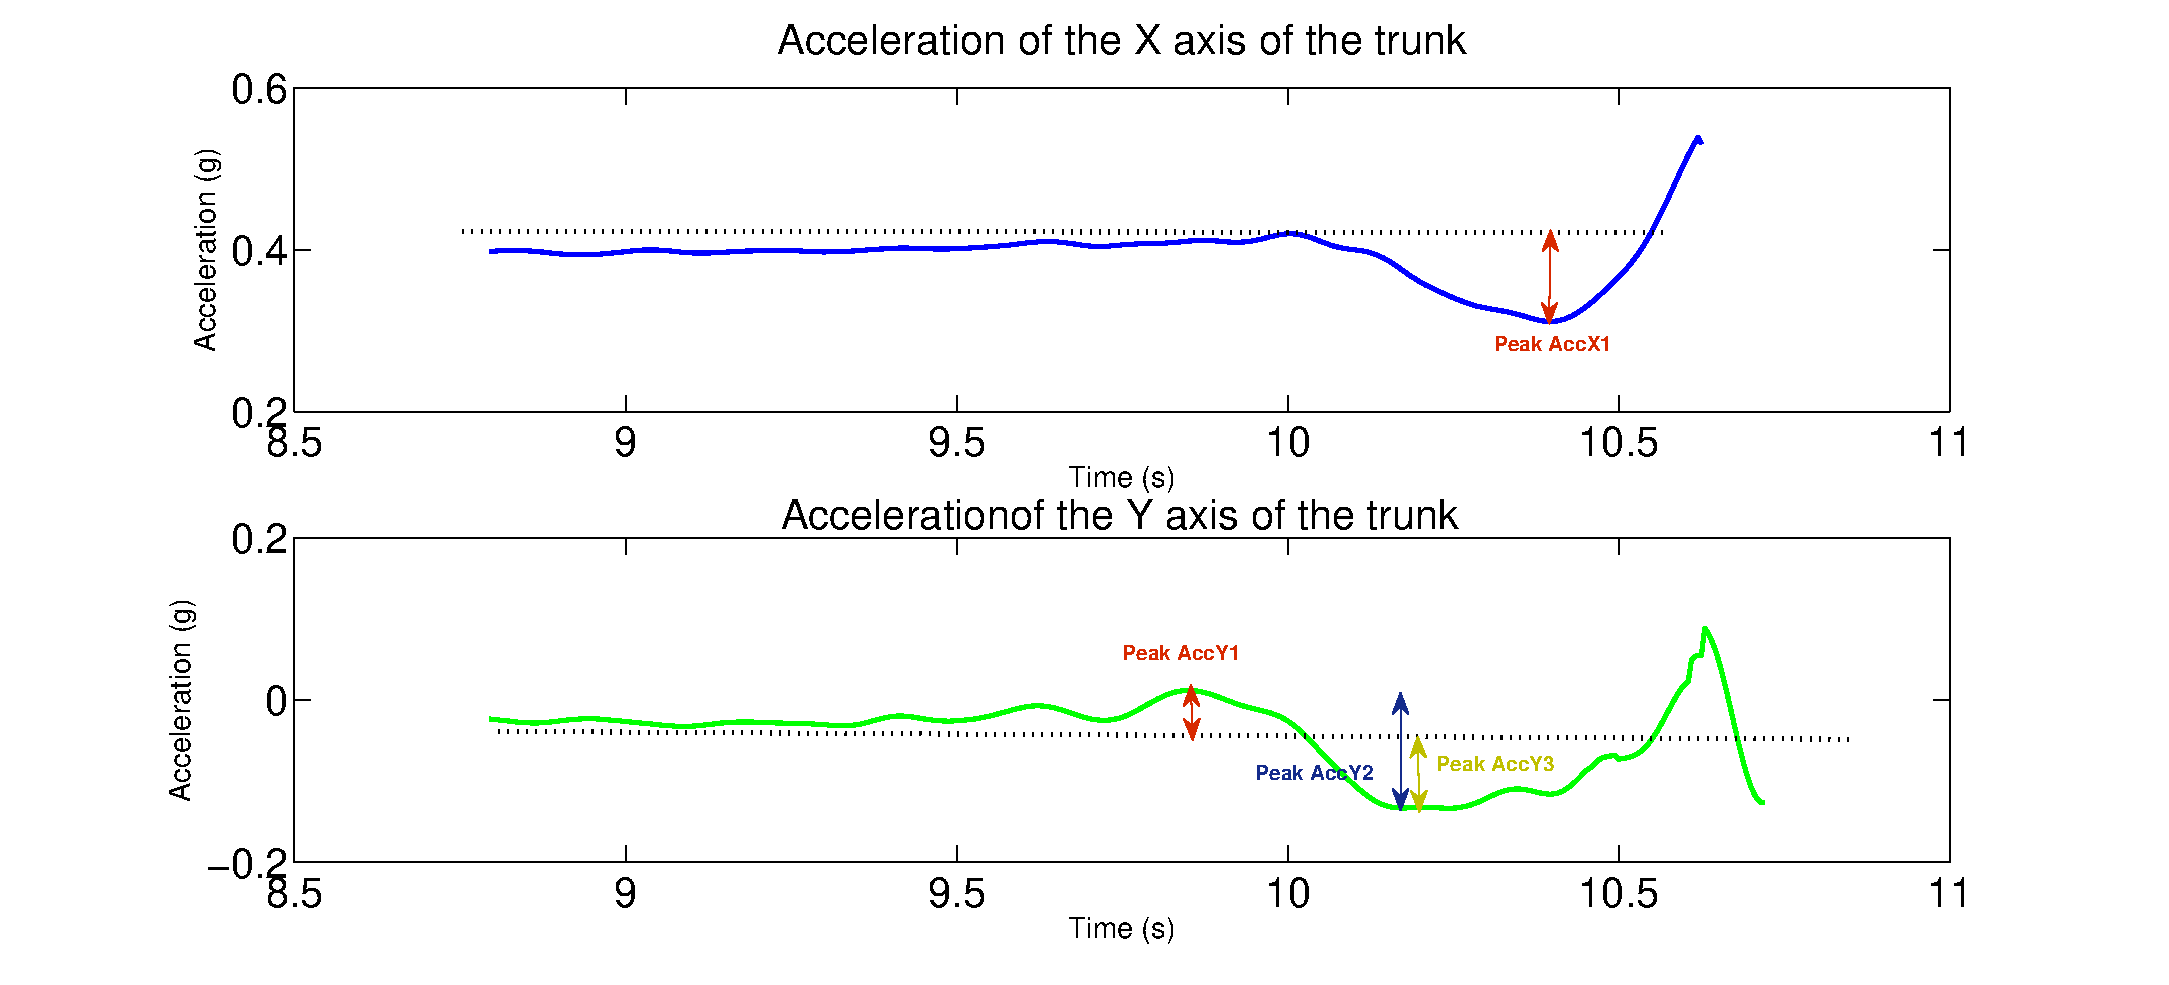
\epsfig{file=figures/Feature_extraction/Acc_features, width=18cm}
	\caption{Peaks in the Acceleration signals .}
	\label{fig:Acc_features}
\end{figure}

\begin{figure}[H]
	\centering
	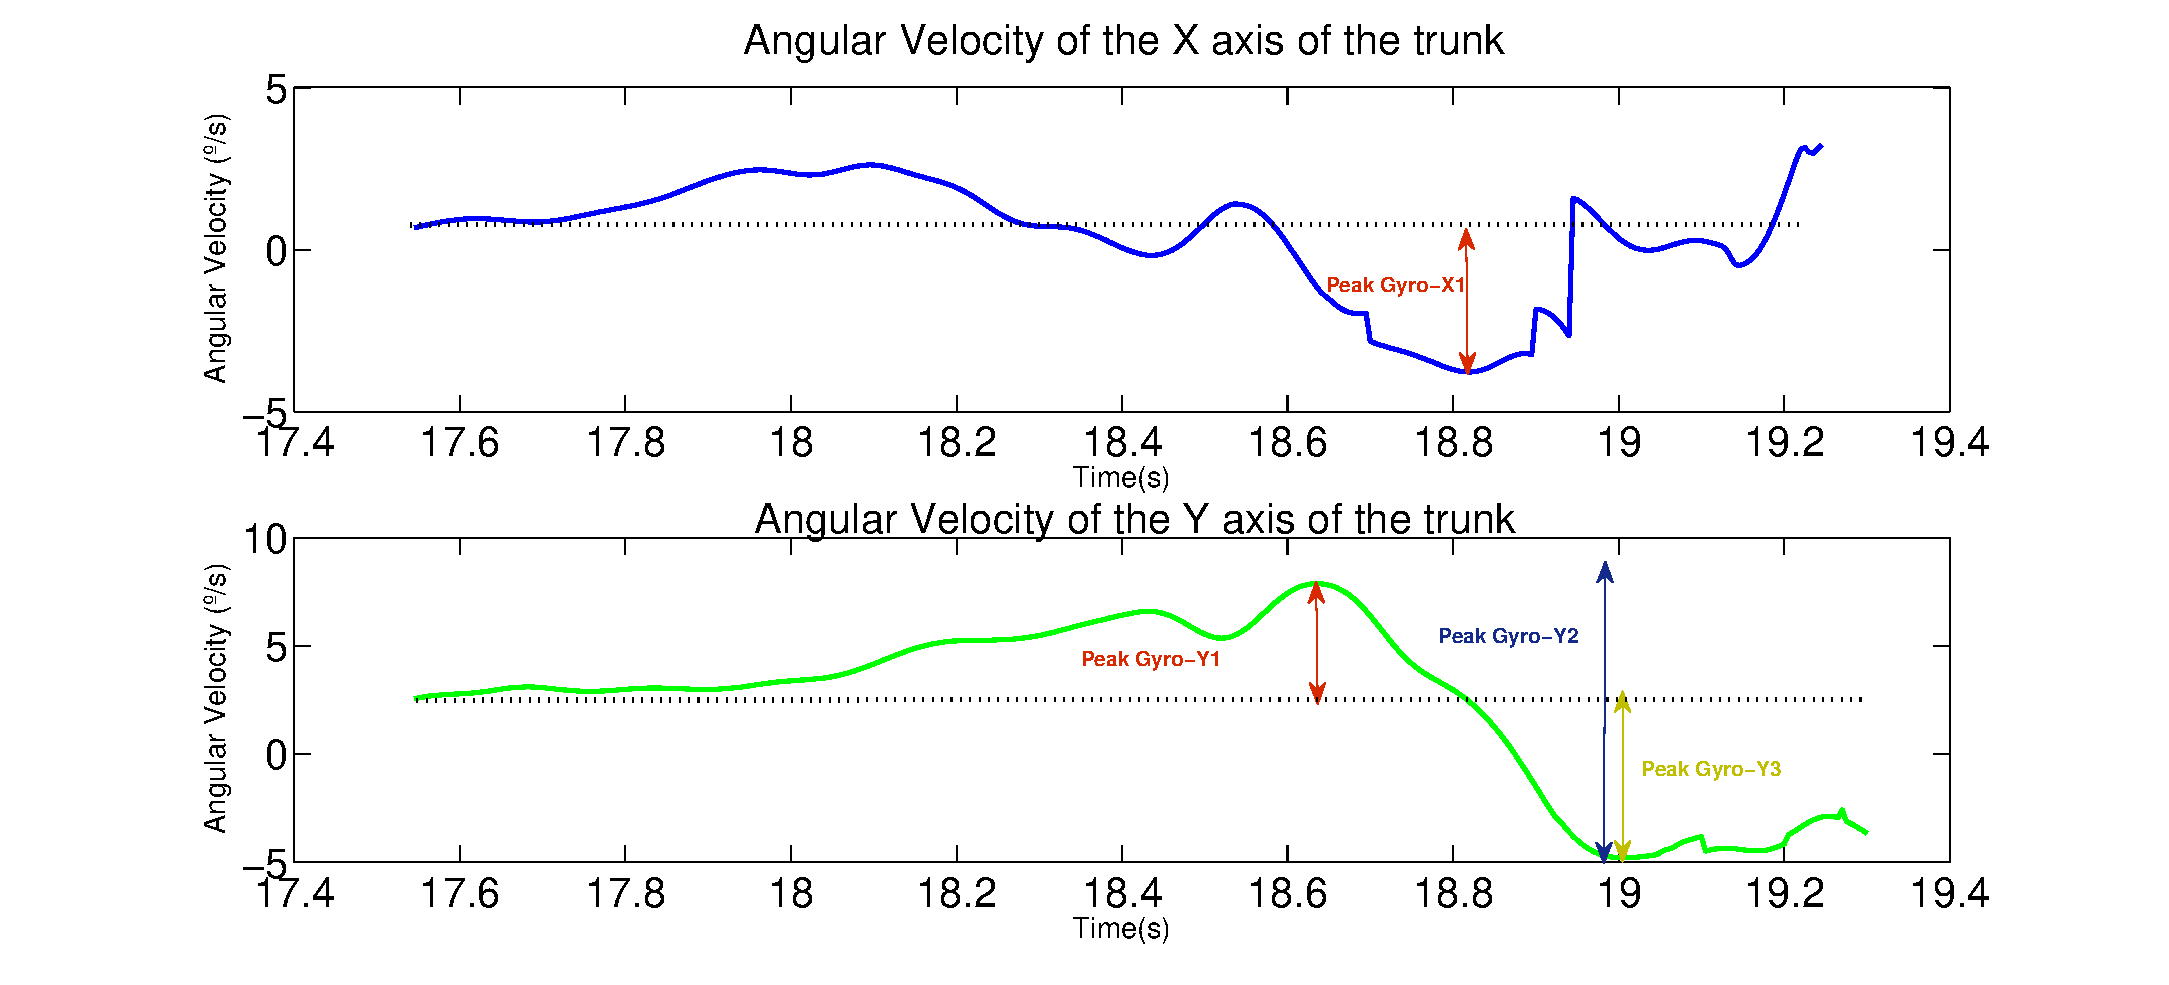
\epsfig{file=figures/Feature_extraction/Gyro_features, width=18cm}
	\caption{Peaks in the Gyroscope signals.}
	\label{fig:Gyro_features}
\end{figure}


Hereafter, we will calculated the APA duration in each system because it would be able to be a appropiate parameter to compare. Also, the majority of these features have been used in others studies \cite{Mancini2009} so it can be a right way to measure the movement.

Now, we are going to apply PCA algorithms to obtain the most significant information about human movement. This method allows us to minimise the redundant information performing the dimensional reduction.

We applied PCA twice: in the signals of the Antero-posterior direction (AP-COP, X-Acc and X-Velocity) and of the Medio-lateral direction (ML-COP, Y-Acc and Y-Velocity). So far, we have the projection in the orthogonal space, three eigenvectors and three eigenvalues. The corresponding eigenvectors are ranked in a descending order of eigen values and by choosing the two first eigenvectors PCA directly performs the dimensional reduction, that is, the class of three dimensional gait data is described by low-dimensional features containing only two principal components.

The two first eigenvalues of the covariance matrix accounts for 98\% of the variance. This indicates that we only need to take the two first eigenvector to have the significant information of the data. Also, if we see \ref{fig:PCA_AP} \ref{fig:PCA_ML}  we can determine that the important information, i.e the information with more variance is defined with the COP and Angular Velocity signals. This is because the acceleration and angular velocity signals are very similar and one of them is not necessary, i.e it does not give us added useful information.
\begin{figure}[H]
	\centering
	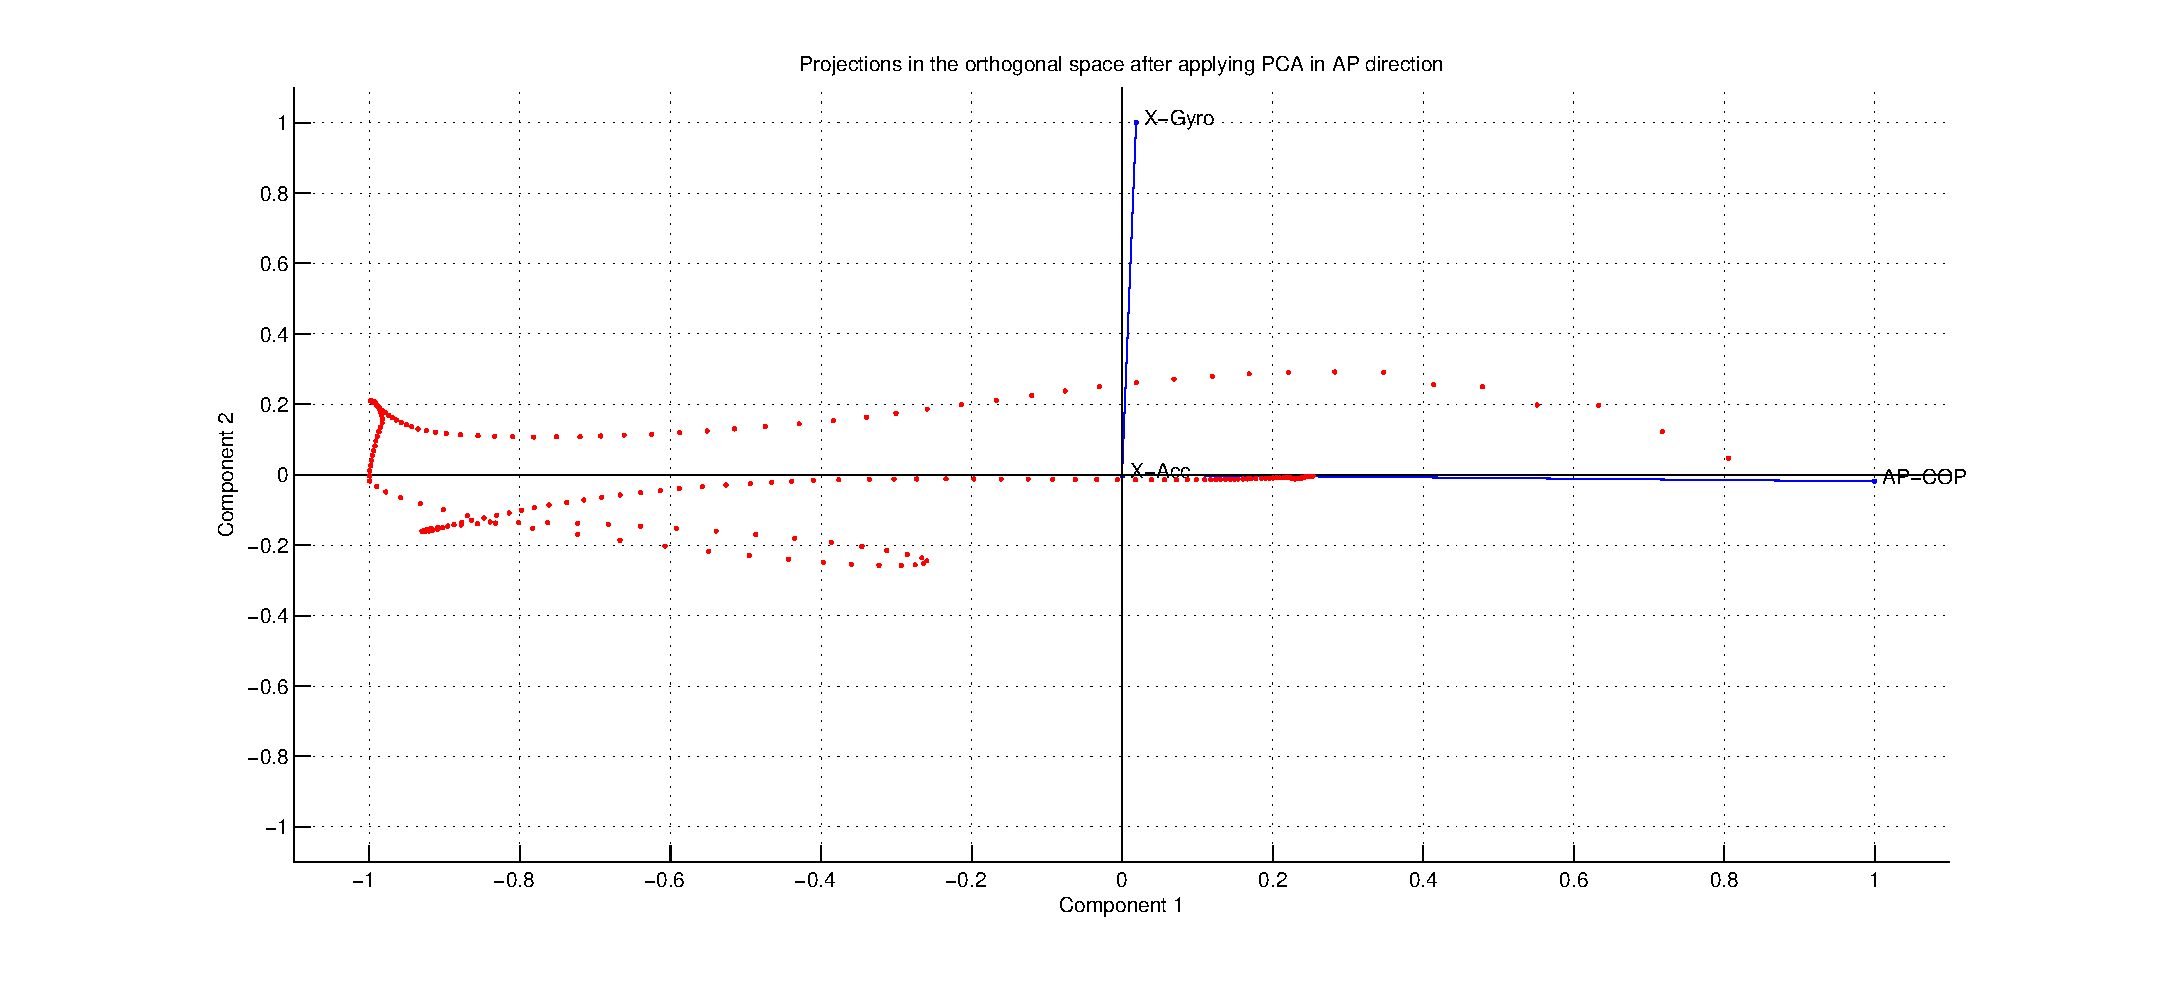
\epsfig{file=figures/Feature_extraction/PCA_AP, width=18cm}
	\caption{Projections in the orthogonal space after applying PCA and eigenvectors in Antero-posterior direction.}
	\label{fig:PCA_AP}
\end{figure}

\begin{figure}[H]
	\centering
	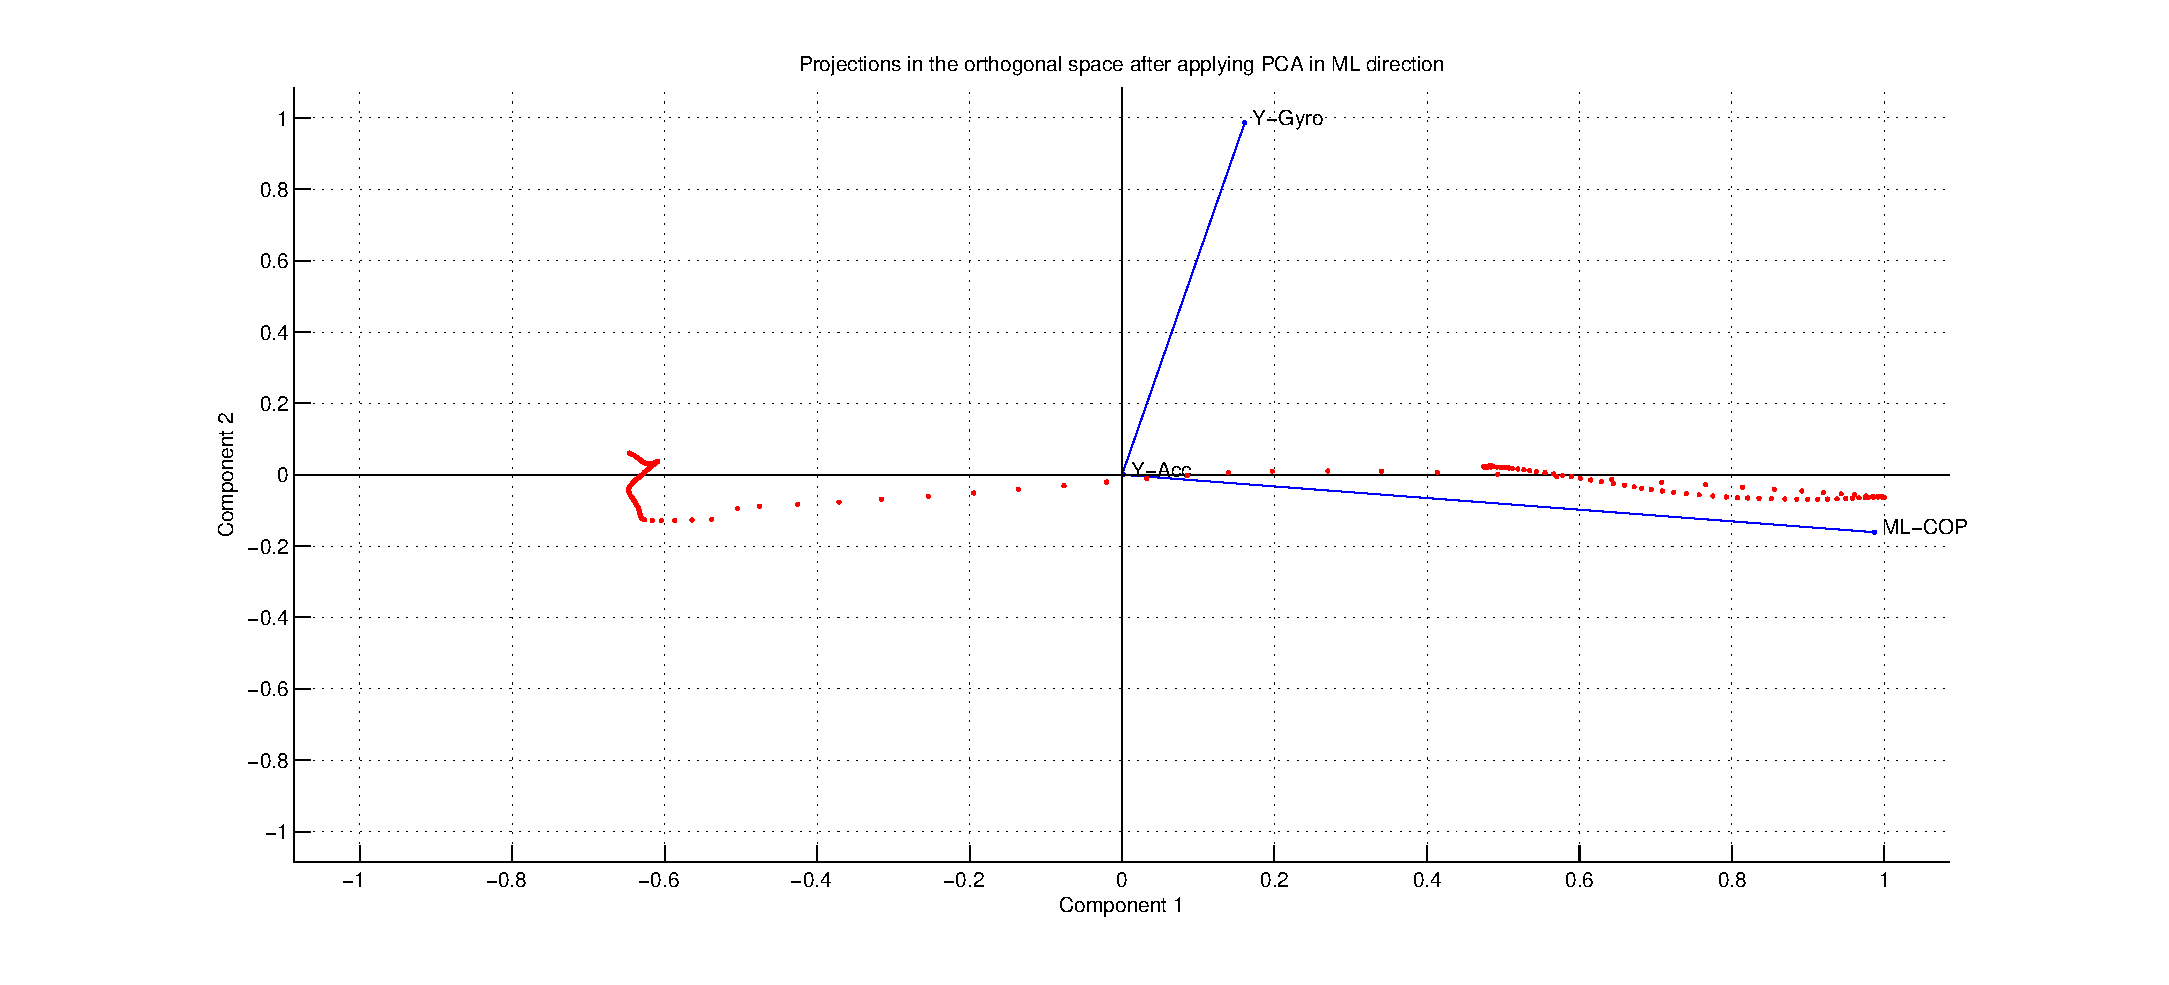
\epsfig{file=figures/Feature_extraction/PCA_ML, width=18cm}
	\caption{Projections in the orthogonal space after applying PCA and eigenvectors in Medio-Lateral direction.}
	\label{fig:PCA_ML}
\end{figure}

The next step is to obtain the same features of the new signals. Now, we have four signals per patient: two components for AP direction and two ones more for ML direction. The characteristics extracted in this case are the same than with the originals signals.

Finally, we apply PCA between patients. Our data base is reduced because we only have five patient. So, our matrix data has five columns where each one has the COP, Acceleration and Angular Velocity concatenated. As in the above study, the two first components account the most of variability and this representation in the space indicates us the movement relation between patients, i.e whether the movement is similar between them. This allows us to know if it is possible to do a classification afterwards and what components are appropriated to do it.
In the Antero-Posterior direction, the projections are located in the right part of the orthogonal space. People analysed in this study are patients with different level of the disease. Therefore, the second component would be able to be useful to differentiate patients with parkinson’s disease. Also, it is possible that the first component can be used to differentiate between control subjects and do a classification \ref{fig:PCA_AP_patients}.

In the Medio-Lateral direction the data are more dispersed. This indicate that the movement changes a lot between patients. However, almost all eigenvectors are pointing toward the upper half of the space\ref{fig:PCA_ML_patients}.

\begin{figure}[H]
	\centering
	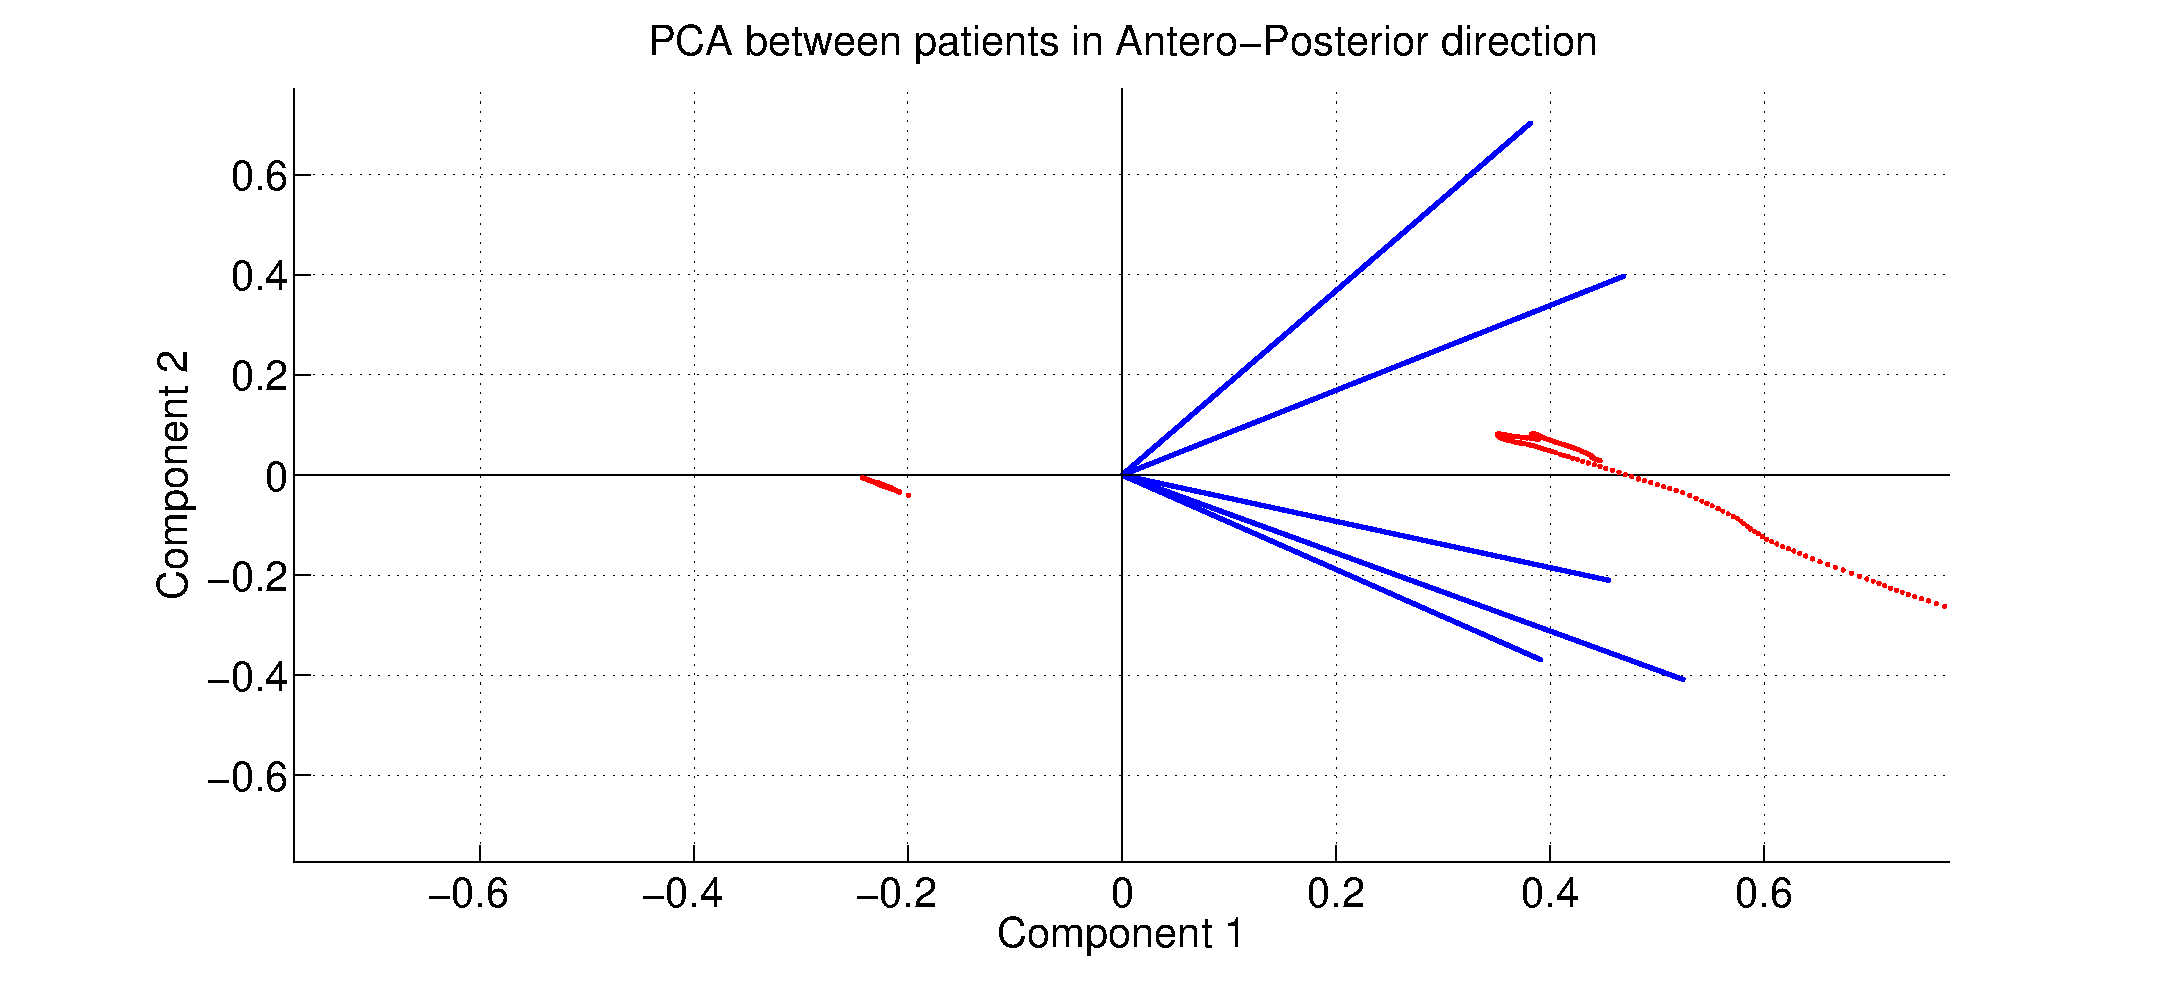
\epsfig{file=figures/Feature_extraction/PCA_AP_patients, width=18cm}
	\caption{Projections in the orthogonal space after applying PCA and eigenvectors in Antero-posterior direction between patients.}
	\label{fig:PCA_AP_patients}
\end{figure}

\begin{figure}[H]
	\centering
	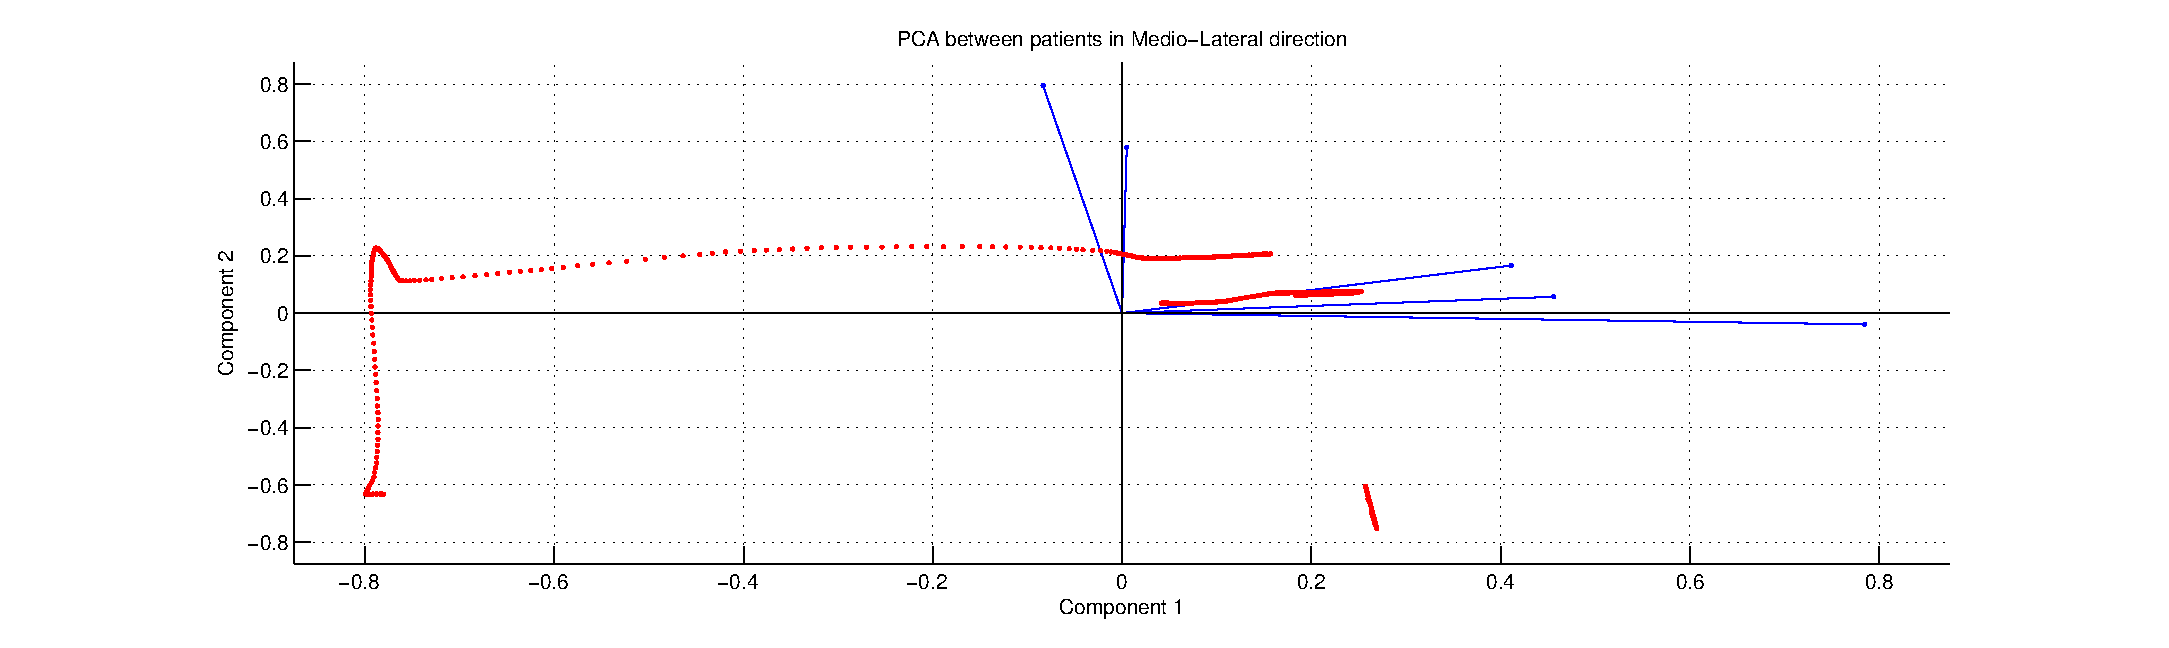
\epsfig{file=figures/Feature_extraction/PCA_ML_patients, width=18cm}
	\caption{Projections in the orthogonal space after applying PCA and eigenvectors in Medio-Lateral direction between patients.}
	\label{fig:PCA_ML_patients}
\end{figure}


\subsection{Results discurssion}
One the APA features have been calculated, we will do the correlation between them. Firstly we are going to do a comparative study between FP and GW in the Antero-posterior direction. We calculated the correlation between the APA peaks detected in the COP signal \ref{fig:COP_features} and the the peak calculated in the acceleration and angular velocity signals \ref{fig:Acc_features}\ref{fig:Gyro_features}. The results of this correlation are showed in \ref{fig:Corr_AP}. If we analyse these values of correlation, we can determine that the feature of the gyroscope have a higher correlation with the features of the COP signal. The first peak of the COP and the peak of acceleration and angular velocity signals account a positive correlation with a significant value. Also, in the center of pressure, the most interesting feature is the first peak, i.e when patient has momentum to step because the correlation with the acceleration signal as well as the angular velocity achieve the highest values.

\begin{figure}[H]
	\centering
	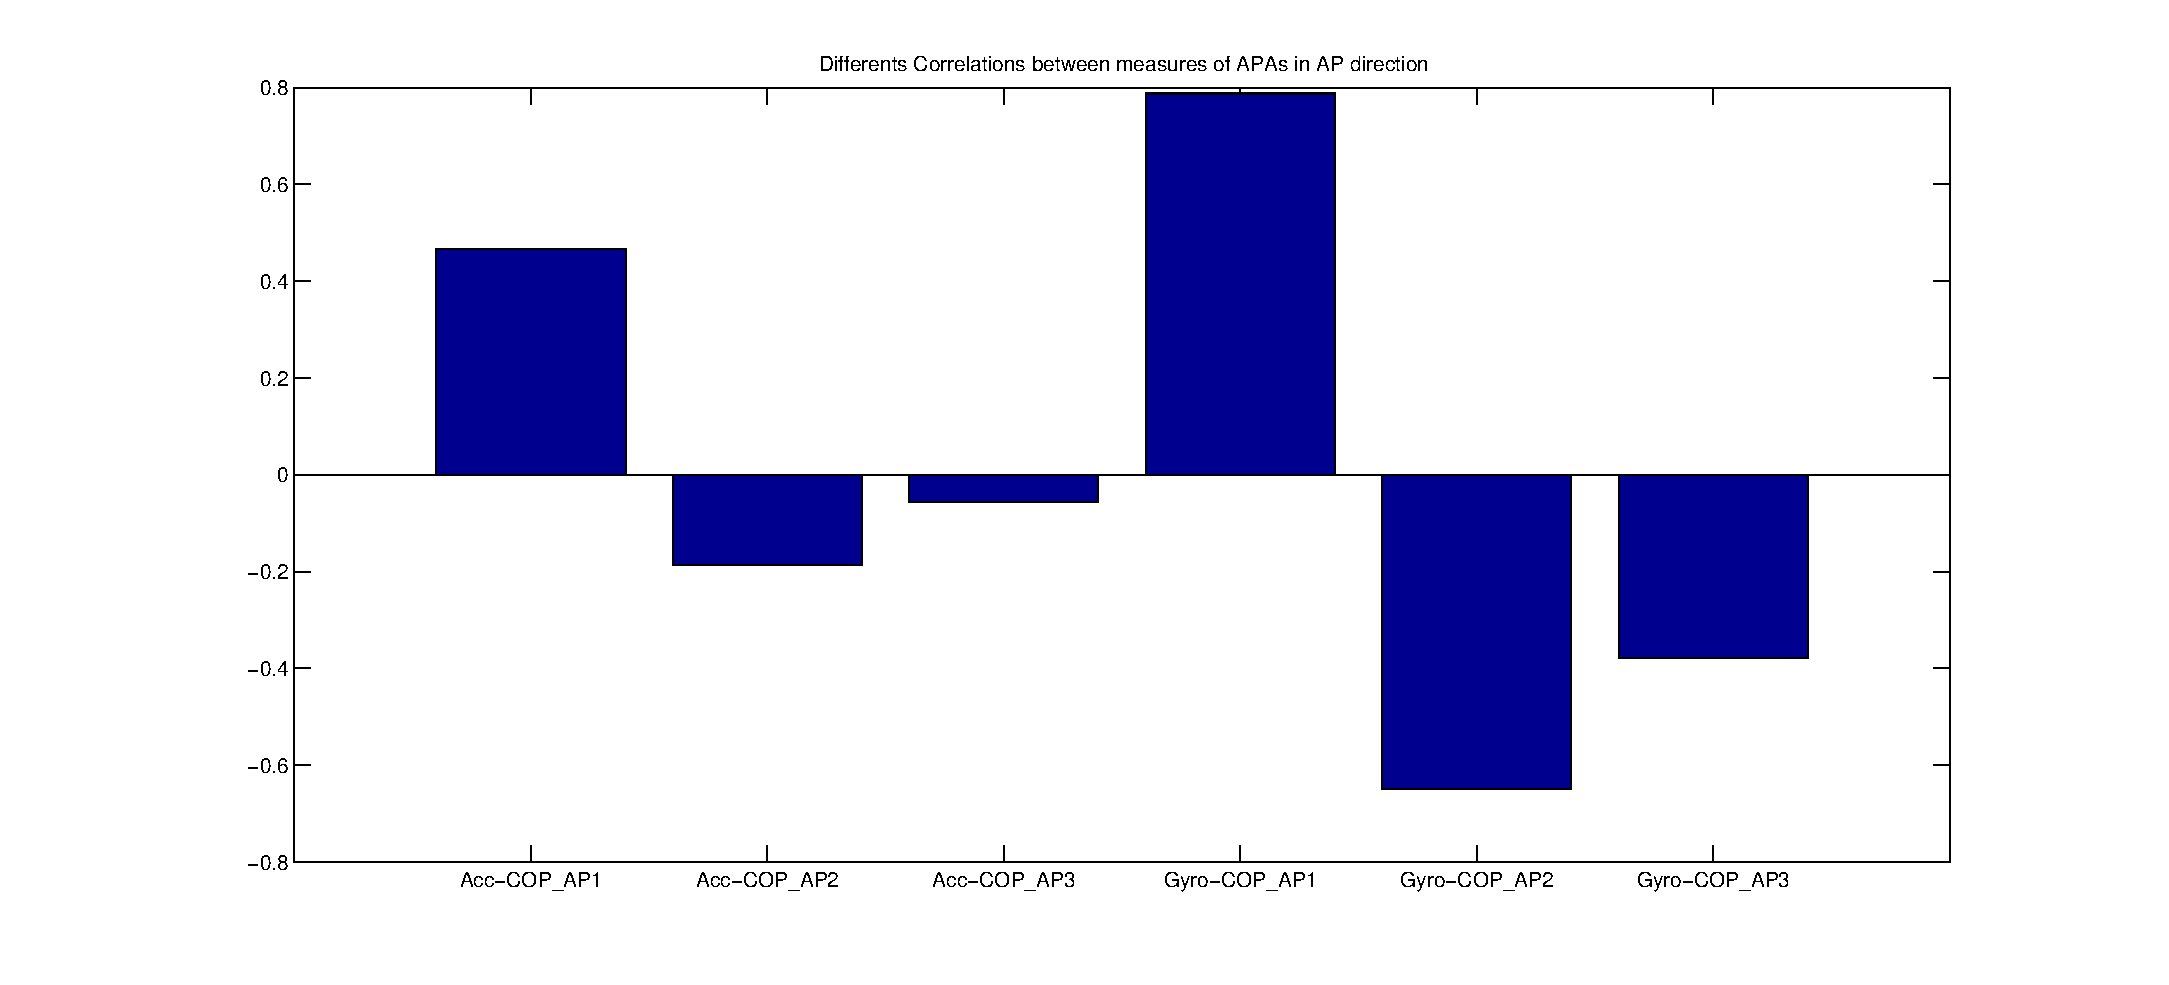
\epsfig{file=figures/Feature_extraction/Corr_AP, width=18cm}
	\caption{Correlation between features in the AP direction.}
	\label{fig:Corr_AP}
\end{figure}

\begin{figure}[H]
	\centering
	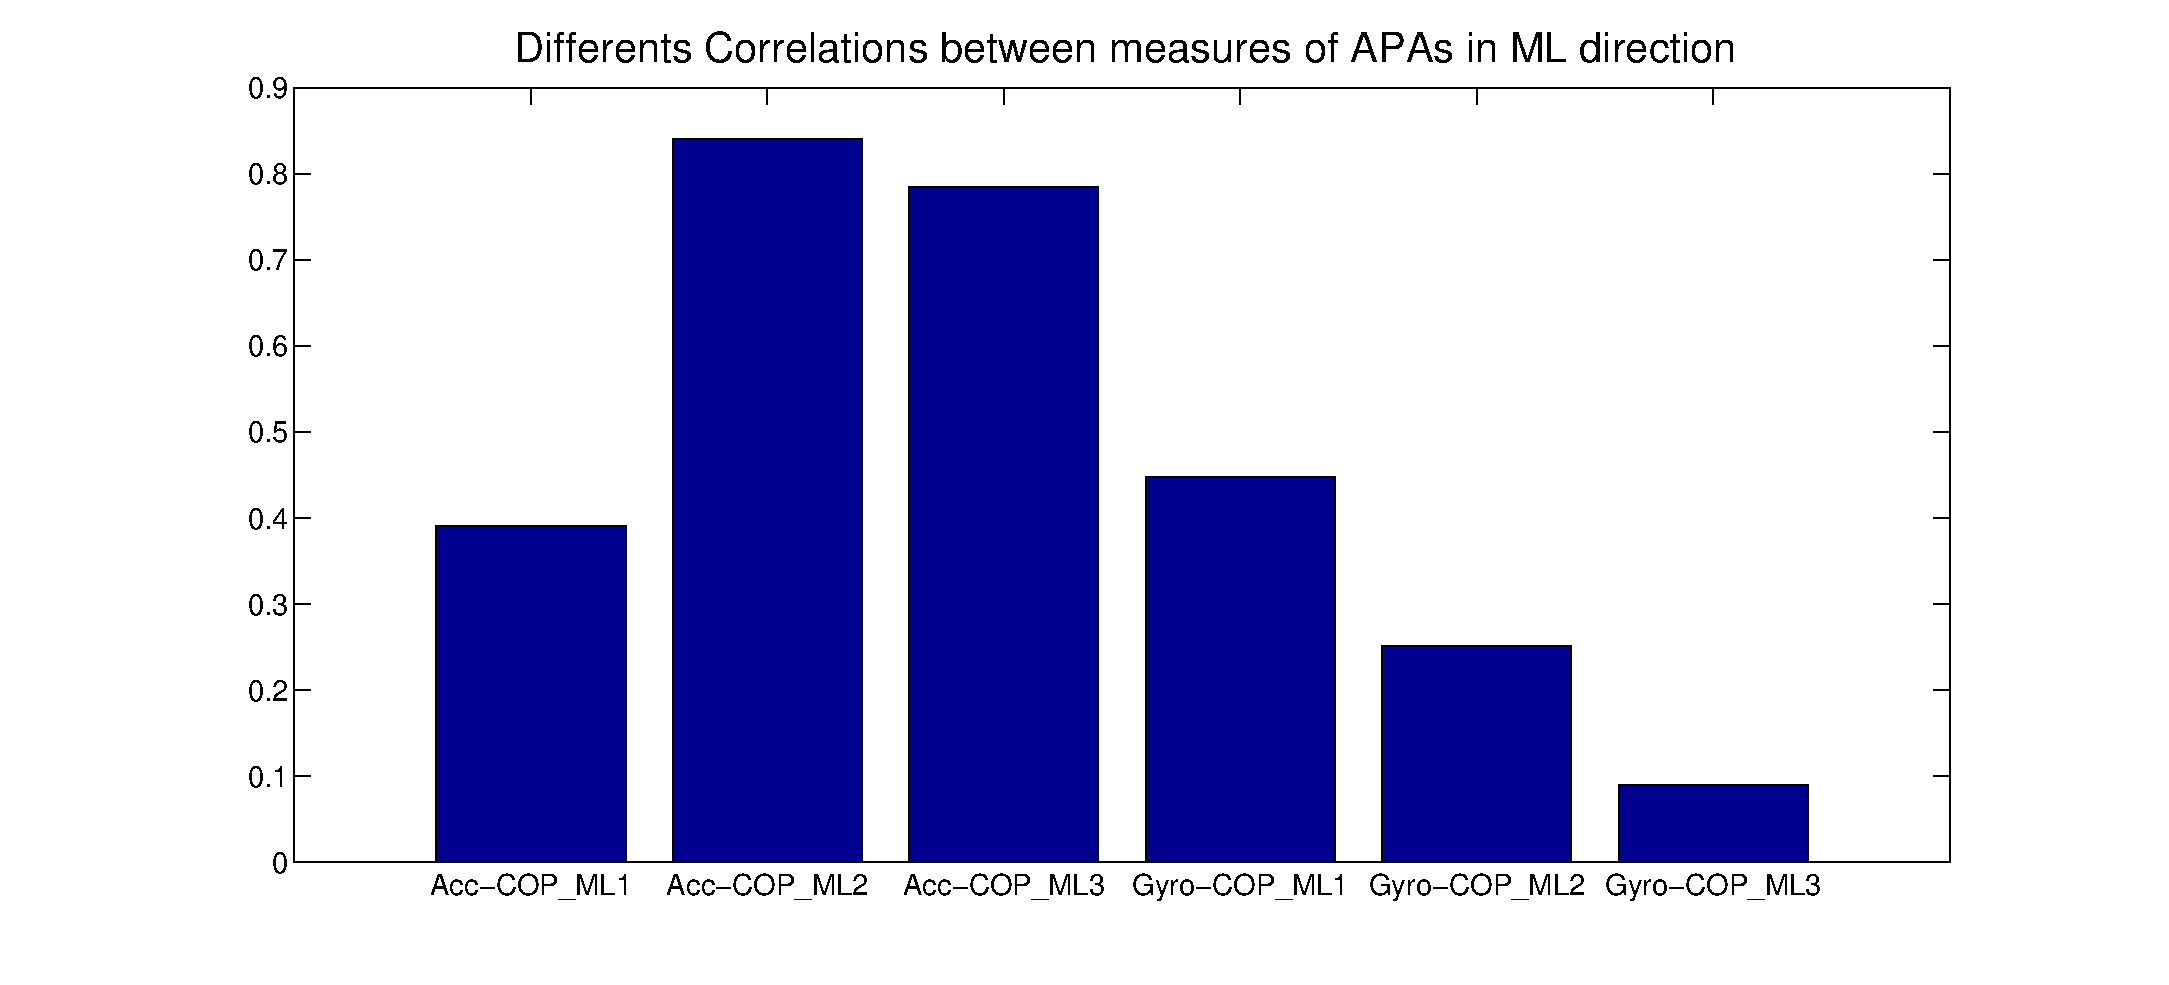
\epsfig{file=figures/Feature_extraction/Corr_ML, width=18cm}
	\caption{Correlation between features in the ML direction.}
	\label{fig:Corr_ML}
\end{figure}

Then, we will compare these signals in the medio-lateral direction. In this case, all correlations are positives and a lot of them with a considerable value. However, we can identify that the most interesting signals in this directions are the signals from the accelerometers. We did the correlation between the peaks detected in the ML-COP and the rest of the features obtained from the acceleration and angular velocity signals. Therefore, the most interesting features of these signals are the height of the negative peak as well as the distance between both peak int he signals \ref{fig:Corr_ML}. The correlation is higher than 0.8, so this indicate that the accelerometers can give us a useful information as the center of pressure.

If we pay attention in the APA duration\ref{fig:Corr_duration}, the correlation between COP and Acceleration and COP and Angular Velocity is negative. This doesn't make sense because it should be positive. Thus, we determine that there is not correlation between them. Even so, there is correlation between the APA duration in accelerometers and gyroscopes.
\begin{figure}[H]
	\centering
	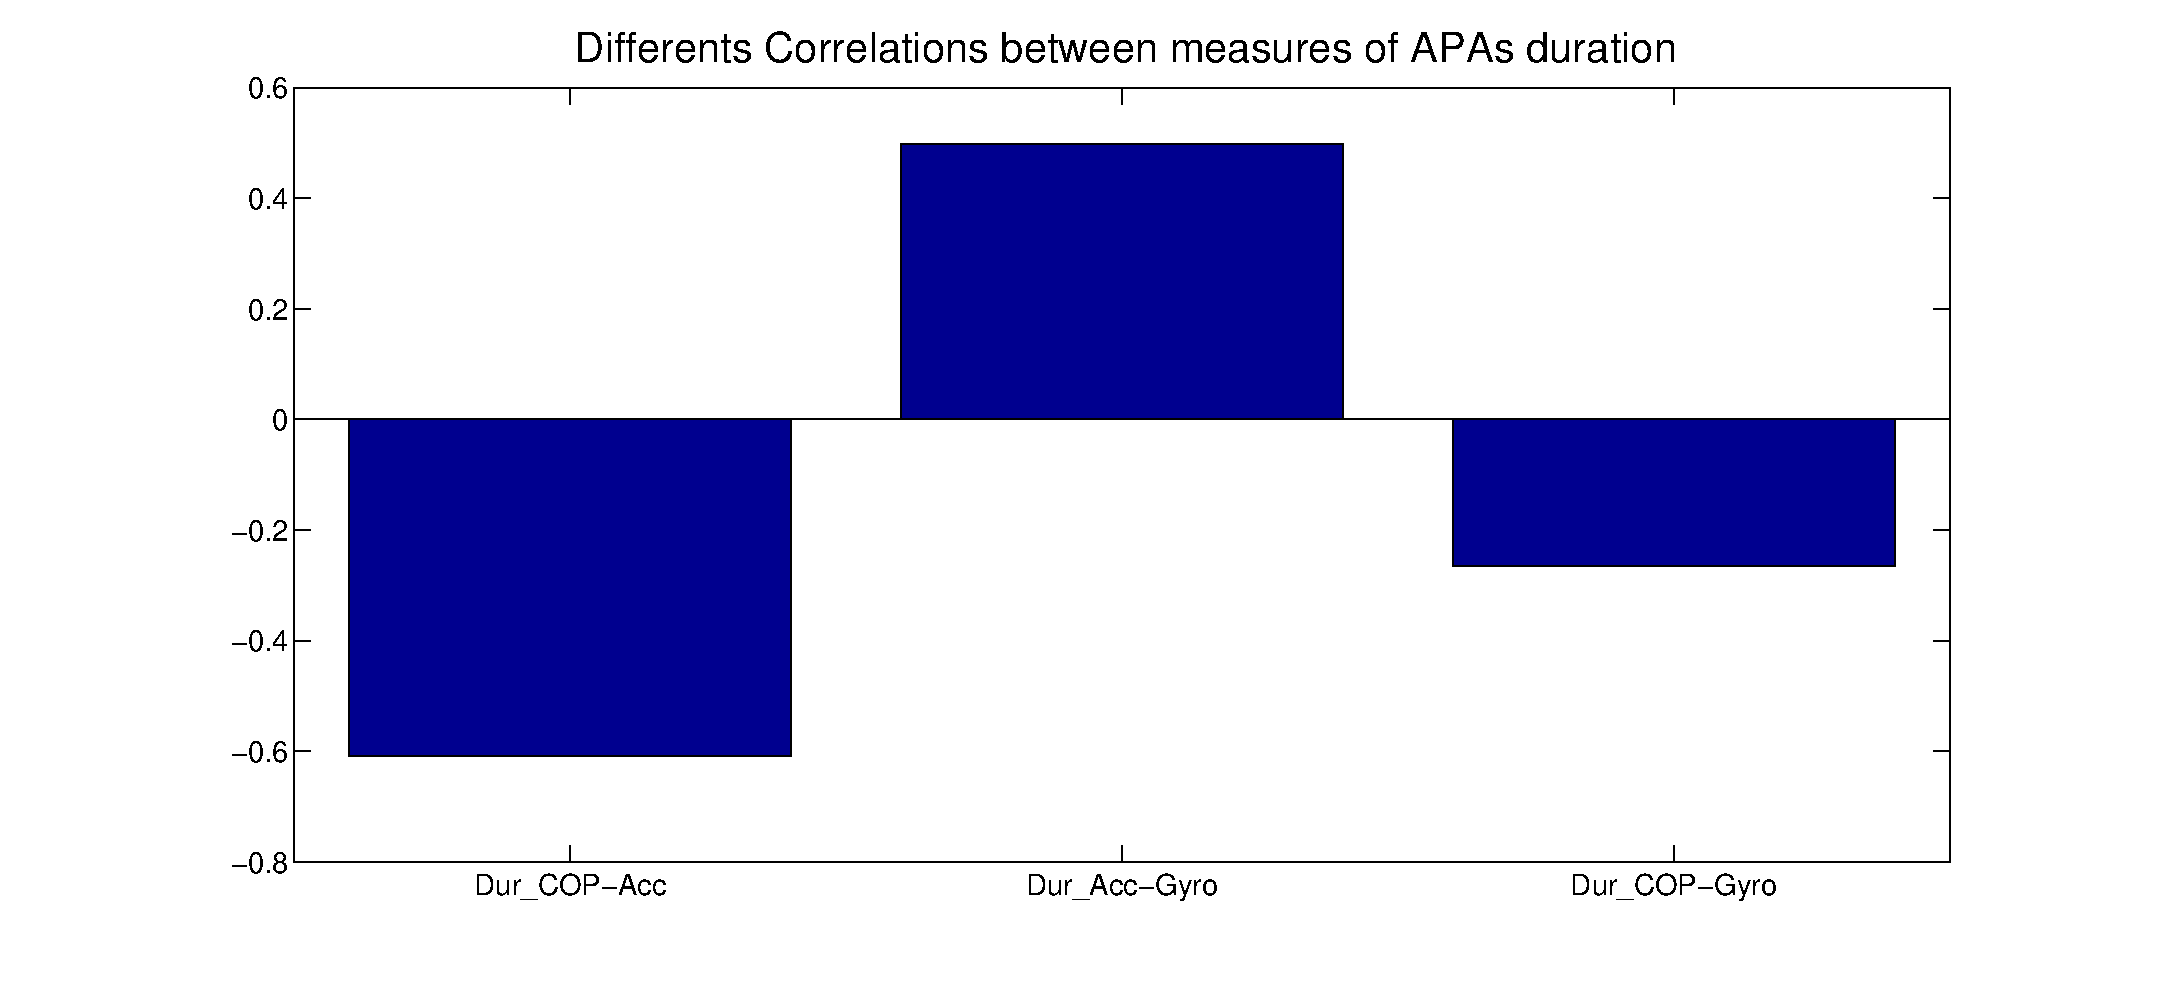
\epsfig{file=figures/Feature_extraction/Corr_duration, width=18cm}
	\caption{Correlation between APA duration.}
	\label{fig:Corr_duration}
\end{figure}

Finally, we are going to see the correlation after using the PCA method. In principle, these features are more accurate because we removed the useful information and we have less and more interesting data.
Whether we observe \ref{fig:Corr_PCA}, the first three values are the correlation between the three APA peaks detected in the first component (analogous to COP signal) and the APA peak of the second component (analogous to angular velocity or acceleration signal) in the AP direction. The most significant value is the correlation between the negative peak in the first component and the peak of the second component.

In the ML direction, we do the correlation between the APA peak of the first component and the three features of the second component. The higher values is the correlation between the peak of the first component and the distance between both peaks of the second component being this a negative correlation\ref{fig:Corr_PCA}.

\begin{figure}[H]
	\centering
	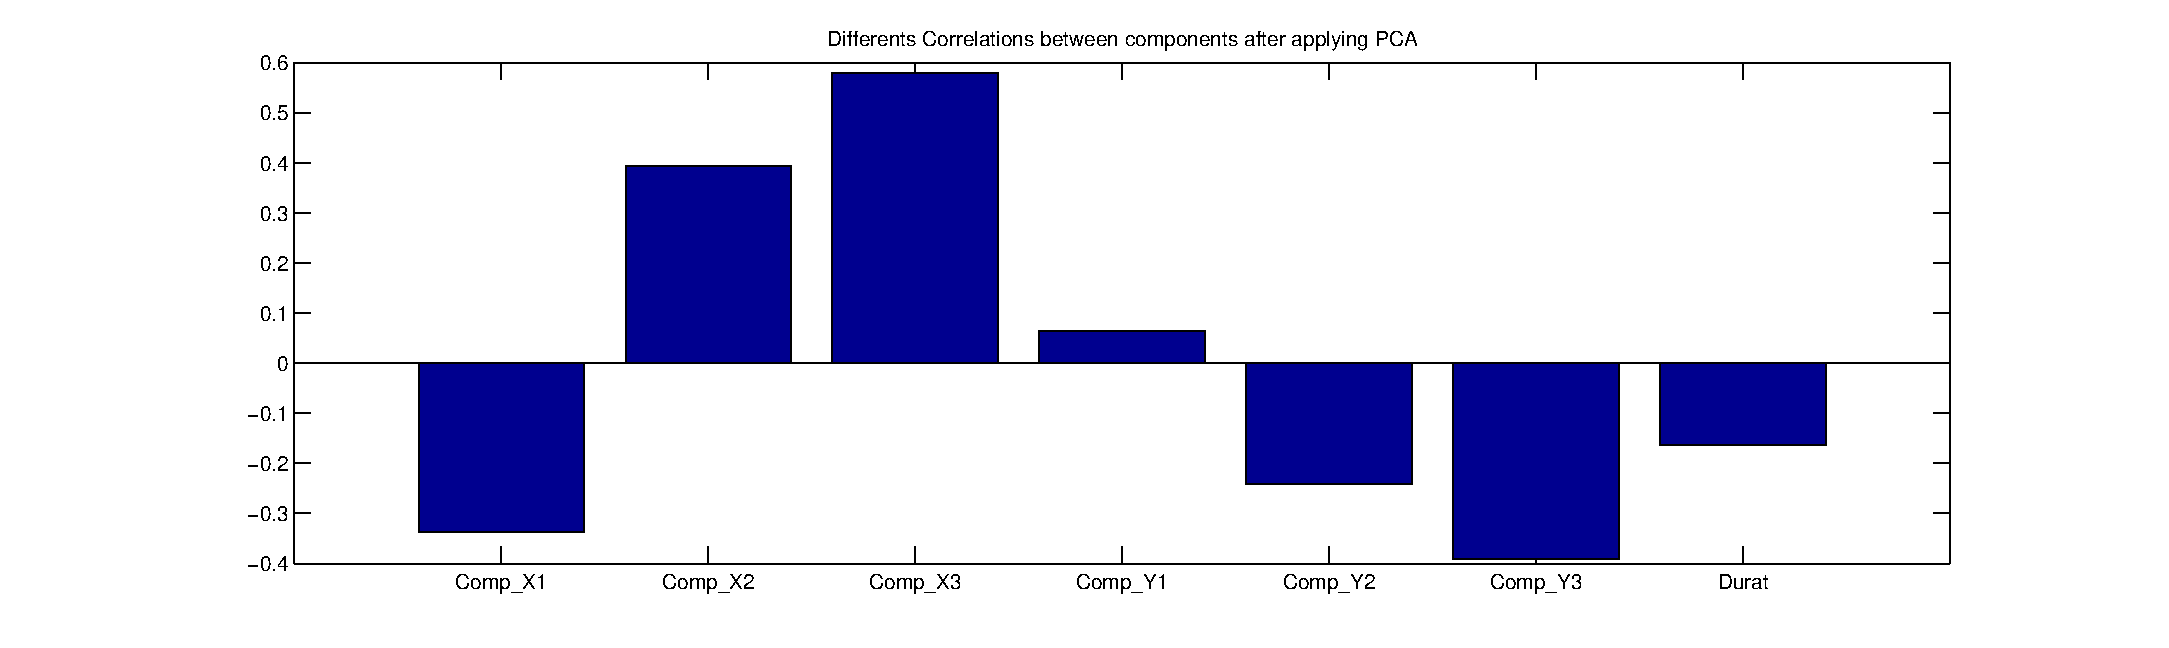
\epsfig{file=figures/Feature_extraction/Corr_PCA, width=18cm}
	\caption{Correlation between features after applying PCA.}
	\label{fig:Corr_PCA}
\end{figure}